%% Created by Maple 2017.3, Windows 10
%% Source Worksheet: MotoModel.mw
%% Generated: Sat Jan 25 19:36:03 CET 2020
\documentclass{article}
\usepackage{maplestd2e}
\def\emptyline{\vspace{12pt}}
\begin{document}
\pagestyle{empty}
\DefineParaStyle{Maple Bullet Item}
\DefineParaStyle{Maple Heading 1}
\DefineParaStyle{Maple Warning}
\DefineParaStyle{Maple Heading 4}
\DefineParaStyle{Maple Heading 2}
\DefineParaStyle{Maple Heading 3}
\DefineParaStyle{Maple Dash Item}
\DefineParaStyle{Maple Error}
\DefineParaStyle{Maple Title}
\DefineParaStyle{Maple Text Output}
\DefineParaStyle{Maple Normal}
\DefineCharStyle{Maple 2D Output}
\DefineCharStyle{Maple 2D Input}
\DefineCharStyle{Maple Maple Input}
\DefineCharStyle{Maple 2D Math}
\DefineCharStyle{Maple Hyperlink}
\begin{center}
\begin{Maple Normal}{
\begin{center}
\begin{Maple Normal}{
\raisebox{1.3611111111111112in}{
\includegraphics[keepaspectratio,totalheight=4.555555555555555in,angle=-90]{MotoModelimage0.eps}}}\end{Maple Normal}
\end{center}
}\end{Maple Normal}
\end{center}
\begin{maplelatex}\begin{center}
\begin{Maple Normal}{
\textbf{PINS}\textbf{}Solution of Optimal Control Problems}\end{Maple Normal}
\end{center}
\end{maplelatex}
\begin{maplelatex}\begin{Maple Normal}{
University of Trento}\end{Maple Normal}
\end{maplelatex}
\begin{center}
\begin{Maple Title}{
\begin{center}
\begin{Maple Title}{
\textbf{Model of a Motorcycle}}\end{Maple Title}
\end{center}
}\end{Maple Title}
\end{center}
\begin{Maple Normal}{
\begin{Maple Normal}{
}\end{Maple Normal}

\begin{Maple Normal}{
Author: Piazza Mattia}\end{Maple Normal}

}\end{Maple Normal}

\begin{maplegroup}
\begin{Maple Normal}{
Date: 22/01/20}\end{Maple Normal}

\end{maplegroup}
\section{\textbf{DATA}}
\begin{maplegroup}
\begin{mapleinput}
\mapleinline{active}{1d}{motorcycle_data := [

    g                       = 9.807             , # [m/s2]    - gravity acceleration

    #      __    _____   
    #  |  |_ |\symbol{92}|/__ | |_|
    #  |__|__| |\symbol{92}_| | | |

    epsilon                 = 0.428             , # [rad]     - caster angle
    L__b                    = 0.730             , # [m]       - dist. swingarm-steer  
    L__swa                  = 0.535             , # [m]       - lenght swingarm
    x__off                  = 0.034             , # [m]       - offset of the front 

    # wheels radius &               
    # torus radius              
    rf                      = 0.292             , # [m]       -
    rtf                     = 0.0624            , # [m]       -
    rr                      = 0.317             , # [m]       -
    rtr                     = 0.097             , # [m]       -

    #   __      
    #  /   _ |V|
    #  \symbol{92}__(_)| |

    # Rear frame            
    x__Rear                 = 0.230             , # [m]       -
    z__Rear                 = 0.068             , # [m]       -

    # Rider (RF__Rear)               
    x__rdr                  = 0.313             , # [m]       -
    z__rdr                  = 0.504             , # [m]       -

    # Swingarm (RF__eta)                
    x__Swing                = 0.275             , # [m]       -
    z__Swing                = 0.052             , # [m]       -

    # Steer (RF__delta)                 
    x__delta                = 0.0230            , # [m]       - 
    z__delta                = -0.098            , # [m]       -  

    # Front wheel &         
    # Unsprung mass         
    x__fw_un                = -0.029            , # [m]       - 
    z__fw_un                = +0.189            , # [m]       - 

    #  ___    __ _ ______ _ 
    #   | |\symbol{92}||_ |_) |  | |_|
    #  _|_| ||__| \symbol{92} | _|_| |

    # Rear frame inertia    
    m__m                    = 154.4             , # [kg]      -
    Ix__m                   = 10.4              , # [kgm2]    -
    Iy__m                   = 27.0              , # [kgm2]    -
    Iz__m                   = 16.0              , # [kgm2]    -
    Cyz__m                  = 0                 , # [kgm2]    -
    Cxz__m                  = 0                 , # [kgm2]    -
    Cxy__m                  = 0                 , # [kgm2]    -

    # Rider inertia 
    m__rdr                  = 68.5              , # [kg]      -
    Ix__rdr                 = 4.946             , # [kgm2]    -
    Iy__rdr                 = 5.908             , # [kgm2]    -
    Iz__rdr                 = 3.304             , # [kgm2]    -
    Cyz__rdr                = 0                 , # [kgm2]    -
    Cxz__rdr                = 0                 , # [kgm2]    -
    Cxy__rdr                = 0                 , # [kgm2]    -

    # Swingarm inertia              
    m__swa                  = 10.0              , # [kg]      -
    Ix__swa                 = 0.020             , # [kgm2]    -
    Iy__swa                 = 0.800             , # [kgm2]    -
    Iz__swa                 = 0.800             , # [kgm2]    -
    Cyz__swa                = 0                 , # [kgm2]    -
    Cxz__swa                = 0                 , # [kgm2]    -
    Cxy__swa                = 0                 , # [kgm2]    -

    # Steer inertia 
    m__delta                = 8.7500            , # [kg]      -
    Ix__delta               = 0.2870            , # [kgm2]    -
    Iy__delta               = 0.143             , # [kgm2]    -
    Iz__delta               = 0.2063            , # [kgm2]    -
    Cyz__delta              = 0                 , # [kgm2]    -
    Cxz__delta              = 0                 , # [kgm2]    -
    Cxy__delta              = 0                 , # [kgm2]    -

    # Front W inertia   
    m__wf                   = 12                , # [kg] 
    Iy__wf                  = 0.4683            , # [kgm2]    - axial inertia
    Id__wf                  = 0.2160            , # [kgm2]    - diametral inertia (Iz__wf)
    Id__wf                  = 0.2160            , # [kgm2]    - diametral inertia (Ix__wf)
    # Rear W inertia                
    m__wr                   = 16.2              , # [kg]
    Iy__wr                  = 0.664             , # [kgm2]    - axial inertia
    Id__wr                  = 0.333             , # [kgm2]    - diametral inertia (Iz__wr)
    Id__wr                  = 0.333             , # [kgm2]    - diametral inertia (Ix__wr)

    # Unsprum inertia               
    Ix__fw_un               = 0.217             , # [kgm2] 
    Iy__fw_un               = 0.1830            , # [kgm2]
    Iz__fw_un               = 0.068             , # [kgm2]    -      

    #  __ _  _  __ __    
    # |_ / \symbol{92}|_)/  |_     
    # |  \symbol{92}_/| \symbol{92}\symbol{92}__|__    

    # Front suspension  
    k__fs                   = 19620             , # [N/m]     -
    c__fs                   = 1679.7            , # [Ns/m]    -
    s__fs                   = 0.490             , # [m]       - relaxation length
    s__fmax                 = 0.490             , # [m]       - max length susp.
    s__fpre                 = 0.007             , # [m]       - preload spring

    # rear suspension    
    k__rs                   = 147360            , # [N/m]     -
    c__rs                   = 12000             , # [Ns/m]    -
    eta__rs                 = 0                 , # [rad]     - angle of relaxed susp
    eta__max                = -0.165            , # [rad]     - max rotaz swingarm
    a__1                    = +0.13526          , # [m/rad]   - coeff. spring deformation
    a__2                    = -0.1385           , # [m/rad2]  - coeff. spring deformation\symbol{94}2
    a__3                    = -0.0358           , # [m/rad3]  - coeff. spring deformation\symbol{94}3

    # Steer torque  
    C__delta                = -10               , # [Ns/rad]  - steering damping
    K__delta                = 0                 , # [N/rad]   - steering stiffness

    # Aero      
    x__a                    = 0                 , # [m]       - x coor. aerodynamic point 
    z__a                    = 0.8776            , # [m]       - z coor. aerodynamic point
    Ca                      = 0.3               , # [Nm2/s2]  - aerodynamic drag coeff

    # Tyre
    Kp__f                   = 100000            , # [N/m]     - tyre radial stiffness
    Cp__f                   = 70                , # [Ns/m]    - tyre radial stiffness
    Kp__r                   = 130000            , # [N/m]     - tyre radial stiffness
    Cp__r                   = 100                 # [Ns/m]    - tyre radial stiffness
 
]; 

save(motorcycle_data,"MODEL_DATA/motorcycle_data.mpl"):
}{}
\end{mapleinput}
\mapleresult
\begin{maplelatex}
\mapleinline{inert}{2d}{motorcycle_data := [g = 9.807, epsilon = .428, L__b = .730, L__swa = .535, x__off = 0.34e-1, rf = .292, rtf = 0.624e-1, rr = .317, rtr = 0.97e-1, x__Rear = .230, z__Rear = 0.68e-1, x__rdr = .313, z__rdr = .504, x__Swing = .275, z__Swing = 0.52e-1, `x__&delta;` = 0.230e-1, `z__&delta;` = -0.98e-1, x__fw_un = -0.29e-1, z__fw_un = .189, m__m = 154.4, Ix__m = 10.4, Iy__m = 27.0, Iz__m = 16.0, Cyz__m = 0, Cxz__m = 0, Cxy__m = 0, m__rdr = 68.5, Ix__rdr = 4.946, Iy__rdr = 5.908, Iz__rdr = 3.304, Cyz__rdr = 0, Cxz__rdr = 0, Cxy__rdr = 0, m__swa = 10.0, Ix__swa = 0.20e-1, Iy__swa = .800, Iz__swa = .800, Cyz__swa = 0, Cxz__swa = 0, Cxy__swa = 0, `m__&delta;` = 8.7500, `Ix__&delta;` = .2870, `Iy__&delta;` = .143, `Iz__&delta;` = .2063, `Cyz__&delta;` = 0, `Cxz__&delta;` = 0, `Cxy__&delta;` = 0, m__wf = 12, Iy__wf = .4683, Id__wf = .2160, Id__wf = .2160, m__wr = 16.2, Iy__wr = .664, Id__wr = .333, Id__wr = .333, Ix__fw_un = .217, Iy__fw_un = .1830, Iz__fw_un = 0.68e-1, k__fs = 19620, c__fs = 1679.7, s__fs = .490, s__fmax = .490, s__fpre = 0.7e-2, k__rs = 147360, c__rs = 12000, eta__rs = 0, eta__max = -.165, a__1 = .13526, a__2 = -.1385, a__3 = -0.358e-1, `C__&delta;` = -10, `K__&delta;` = 0, x__a = 0, z__a = .8776, Ca = .3, Kp__f = 100000, Cp__f = 70, Kp__r = 130000, Cp__r = 100]}{\[\displaystyle {\it motorcycle\_data}\, := \,[g= 9.807,\epsilon= 0.428,L_{b}= 0.730\\
\mbox{},L_{{\it swa}}= 0.535,x_{{\it off}}= 0.034,{\it rf}\\
\mbox{}= 0.292,{\it rtf}= 0.0624,{\it rr}= 0.317\\
\mbox{},{\it rtr}= 0.097,x_{{\it Rear}\\
\mbox{}}= 0.230,z_{{\it Rear}\\
\mbox{}}= 0.068,x_{{\it rdr}}= 0.313\\
\mbox{},z_{{\it rdr}}= 0.504,x_{{\it Swing}}= 0.275,z_{{\it Swing}}= 0.052\\
\mbox{},x_{\delta }= 0.0230,z_{\delta }=- 0.098,x_{{\it fw\_un}\\
\mbox{}}=- 0.029,z_{{\it fw\_un}\\
\mbox{}}= 0.189,m_{m}= 154.4\\
\mbox{},{\it Ix}_{m}= 10.4,{\it Iy}_{m}= 27.0,{\it Iz}\\
\mbox{}_{m}= 16.0,{\it Cyz}_{m}=0,{\it Cxz}_{m}=0,{\it Cxy}_{m}=0,m_{{\it rdr}}= 68.5\\
\mbox{},{\it Ix}_{{\it rdr}}= 4.946,{\it Iy}_{{\it rdr}}= 5.908,{\it Iz}\\
\mbox{}_{{\it rdr}}= 3.304\\
\mbox{},{\it Cyz}_{{\it rdr}}=0,{\it Cxz}_{{\it rdr}}=0,{\it Cxy}_{{\it rdr}}=0,m_{{\it swa}}= 10.0,{\it Ix}_{{\it swa}}= 0.020,{\it Iy}_{{\it swa}}=\\
\mbox{} 0.800,{\it Iz}\\
\mbox{}_{{\it swa}}= 0.800,{\it Cyz}_{{\it swa}}=0,{\it Cxz}_{{\it swa}}=0,{\it Cxy}_{{\it swa}}=0,m_{\delta }= 8.7500,{\it Ix}_{\delta }=\\
\mbox{} 0.2870,{\it Iy}_{\delta }= 0.143,{\it Iz}\\
\mbox{}_{\delta }= 0.2063,{\it Cyz}_{\delta }=0,{\it Cxz}_{\delta }=0,{\it Cxy}_{\delta }=\\
\mbox{}0,m_{{\it wf}}=12,{\it Iy}_{{\it wf}}= 0.4683,{\it Id}_{{\it wf}}= 0.2160\\
\mbox{},{\it Id}_{{\it wf}}= 0.2160,m_{{\it wr}}= 16.2,{\it Iy}_{{\it wr}}= 0.664\\
\mbox{},{\it Id}_{{\it wr}}= 0.333,{\it Id}_{{\it wr}}= 0.333,{\it Ix}_{{\it fw\_un}\\
\mbox{}}= 0.217,{\it Iy}_{{\it fw\_un}\\
\mbox{}}= 0.1830\\
\mbox{},{\it Iz}\\
\mbox{}_{{\it fw\_un}\\
\mbox{}}= 0.068,k_{{\it fs}}=19620,c\\
\mbox{}_{{\it fs}}= 1679.7,s_{{\it fs}}= 0.490,s_{{\it fmax}}= 0.490\\
\mbox{},s_{{\it fpre}}= 0.007,k_{{\it rs}}=147360,c\\
\mbox{}_{{\it rs}}=12000,\eta\\
\mbox{}_{{\it rs}}=0,\eta\\
\mbox{}_{{\it max}}=- 0.165,a_{1}= 0.13526\\
\mbox{},a_{2}=- 0.1385,a_{3}=- 0.0358,C\\
\mbox{}_{\delta }=-10,K_{\delta }=0,x_{a}=0,z_{a}= 0.8776,{\it Ca}= 0.3,{\it Kp}\\
\mbox{}_{f}=100000,{\it Cp}_{f}=70,{\it Kp}\\
\mbox{}_{r}=130000,{\it Cp}_{r}=100]\]}
\end{maplelatex}
\end{maplegroup}
\begin{maplegroup}
\begin{mapleinput}
\mapleinline{active}{1d}{# Deprecated
}{}
\end{mapleinput}
\end{maplegroup}
\begin{maplegroup}
\begin{mapleinput}
\mapleinline{active}{1d}{simple_tyre_data := [

    #     _  _____ __    __ _  _           _     _  _  __ __       _ 
    # |V||_|/__ | /     |_ / \symbol{92}|_)|V|| ||  |_|   |_)|_|/  |_   ||/ |_|
    # | || |\symbol{92}_|_|_\symbol{92}__   |  \symbol{92}_/| \symbol{92}| ||_||__| |   |  | |\symbol{92}__|__\symbol{92}_||\symbol{92} | |

    #  _  __ _  _ 
    # |_)|_ |_||_)
    # | \symbol{92}|__| || \symbol{92}

    # Rear tyre 
    # METZELER 180/70

    K__P__R                 = 130000            , # [N/m]     - radial stiffness
    C__P__R                 =    100            , # [Ns/m]    - radial damping

    # Long. force               
    Bx__r                   =  13.00            , # []        -       
    Cx__r                   =  1.40             , # []        - (@ KS=23.66)
    Dx__r                   =  1.300            , # []        -         
    Ex__r                   =  0.50             , # []        -

    # Lat. force                
    By__r                   =  3.00             , # []        -       
    Cy__r                   =  2.70             , # []        - (@ KL=12.96 )
    Dy__r                   =  1.60             , # []        -
    Ey__r                   =  0.99             , # []        -
    sigma1__R               =  0.20             , # [m]       - relaxation lenght
    kphi1__R                =  0.650            , # [N/Rad]   - roll stiffness

    # Moments               
    u__r                    =  0.006            , # [m]       - rolling friction parameter
    Mtz__r                  =  0.040            , # [m/Rad]   - 
    LambdaMax__R            =  0.314            , # [N/Rad]   - zero trail
    Tt__r                   = .030              , # [m]       - tyre trail

    #  __ _  _    ___
    # |_ |_)/ \symbol{92}|\symbol{92}| | 
    # |  | \symbol{92}\symbol{92}_/| | | 

    # Front tyre                
    # METZELER 120/70  

    K__P__F                 = 100000            , # [N/m]     - radial stiffness
    C__P__F                 = 70                , # [Ns/m]    - radial damping

    # Long. force               
    Bx__f                   =  13.00            , # []        -
    Cx__f                   =  1.40             , # []        - (@ KS=23.667)
    Dx__f                   =  1.300            , # []        -        
    Ex__f                   =  0.50             , # []        -

    # Lat. force                
    By__f                   =  2.80             , # []        -
    Cy__f                   =  2.50             , # []        - (@ KL=12.96 )
    Dy__f                   =  2.00             , # []        -
    Ey__f                   =  0.95             , # []        -
    sigma1__F               =  0.20             , # [m]       - relaxation lenght
    kphi1__F                =  0.90             , # [N/Rad]   - roll stiffness

    # Moments               
    u__f                    =  0.005            , # [m]       - rolling friction parameter
    Mtz__f                  =  0.045            , # [m/Rad]   -
    LambdaMax__F            =  0.279            , # [N/Rad]   - zero trail
    Tt__f                   =  0.020              # [m]       - tyre trail
    
];

save(simple_tyre_data ,"MODEL_DATA/tyre_data_linear.mpl"):
}{}
\end{mapleinput}
\mapleresult
\begin{maplelatex}
\mapleinline{inert}{2d}{simple_tyre_data := [K__P__R = 130000, C__P__R = 100, Bx__r = 13.00, Cx__r = 1.40, Dx__r = 1.300, Ex__r = .50, By__r = 3.00, Cy__r = 2.70, Dy__r = 1.60, Ey__r = .99, `&sigma;1__R` = .20, kphi1__R = .650, u__r = 0.6e-2, Mtz__r = 0.40e-1, LambdaMax__R = .314, Tt__r = 0.30e-1, K__P__F = 100000, C__P__F = 70, Bx__f = 13.00, Cx__f = 1.40, Dx__f = 1.300, Ex__f = .50, By__f = 2.80, Cy__f = 2.50, Dy__f = 2.00, Ey__f = .95, `&sigma;1__F` = .20, kphi1__F = .90, u__f = 0.5e-2, Mtz__f = 0.45e-1, LambdaMax__F = .279, Tt__f = 0.20e-1]}{\[\displaystyle {\it simple\_tyre\_data}\, := \,[K_{P_{R}}=130000,C_{P_{R}}=100,{\it Bx}_{r}= 13.0,{\it Cx}_{r}=\\
\mbox{} 1.40,{\it Dx}_{r}= 1.300,{\it Ex}_{r}= 0.50\\
\mbox{},{\it By}_{r}= 3.0,{\it Cy}_{r}= 2.70,{\it Dy}_{r}= 1.60\\
\mbox{},{\it Ey}_{r}= 0.99,\sigma \mbox {{\tt `1`}}\\
\mbox{}_{R}= 0.20,{\it kphi1}\\
\mbox{}_{R}= 0.650,u_{r}= 0.006,{\it Mtz}_{r}= 0.040\\
\mbox{},{\it LambdaMax}_{R}= 0.314,{\it Tt}_{r}= 0.030\\
\mbox{},K_{P_{F}}=100000,C_{P_{F}}=70,{\it Bx}_{f}= 13.0,{\it Cx}_{f}= 1.40,{\it Dx}_{f}= 1.300\\
\mbox{},{\it Ex}_{f}= 0.50,{\it By}_{f}= 2.80,{\it Cy}_{f}= 2.50,{\it Dy}_{f}= 2.0,{\it Ey}_{f}= 0.95\\
\mbox{},\sigma \mbox {{\tt `1`}}\\
\mbox{}_{F}= 0.20,{\it kphi1}\\
\mbox{}_{F}= 0.90,u_{f}= 0.005\\
\mbox{},{\it Mtz}_{f}= 0.045,{\it LambdaMax}_{F}= 0.279,{\it Tt}_{f}= 0.020]\]}
\end{maplelatex}
\end{maplegroup}
\section{\textbf{CURVILINEAR COORDINATES}}
\begin{maplegroup}
\begin{Maple Normal}{
\textbf{TAKEN FROM DA LIO MODEL}}\end{Maple Normal}

\end{maplegroup}
\begin{maplegroup}
\begin{Maple Normal}{
Coordinates and symbols}\end{Maple Normal}

\end{maplegroup}
\begin{maplegroup}
\begin{Maple Normal}{
\raisebox{6.416666666666667in}{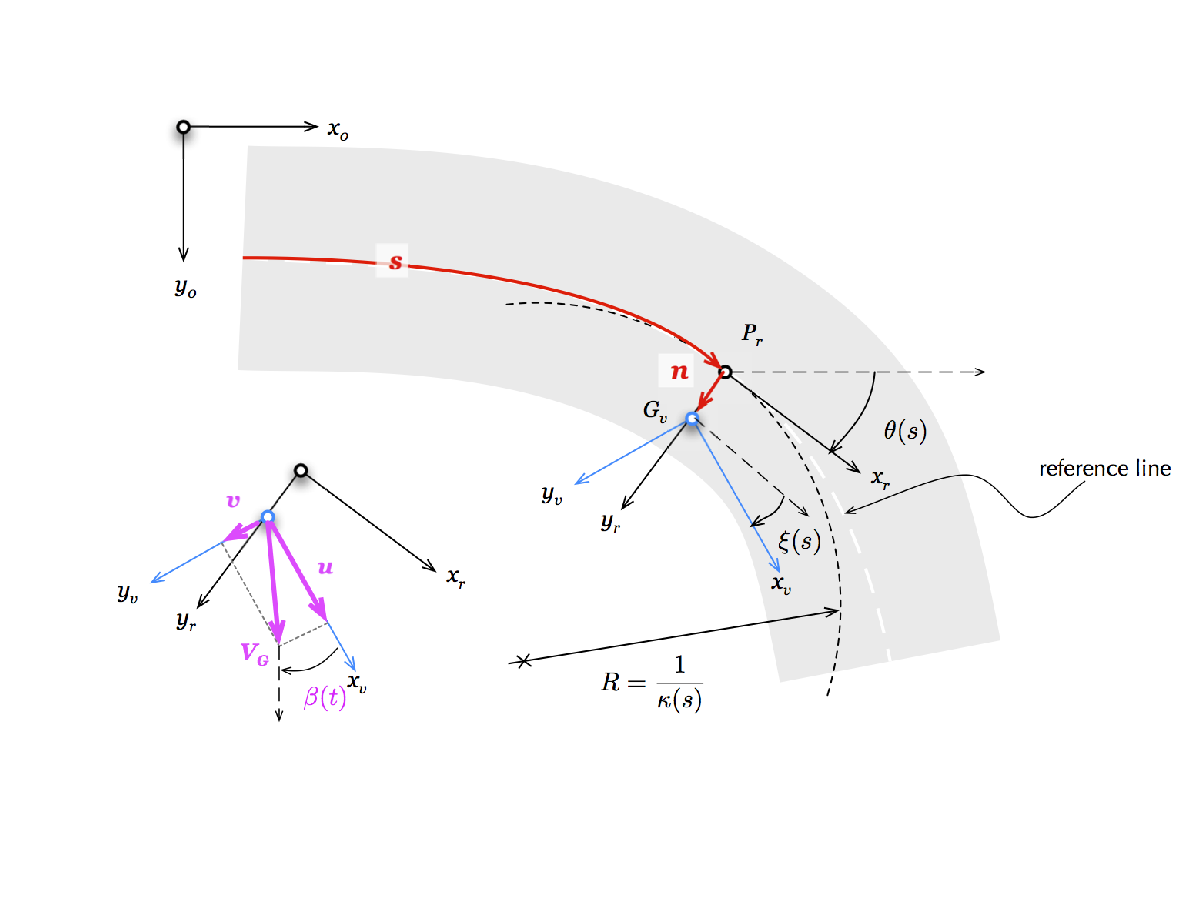
\includegraphics[keepaspectratio,totalheight=8.583333333333334in,angle=-90]{MotoModelimage1.eps}}}\end{Maple Normal}
\end{maplegroup}
\begin{maplegroup}
\begin{Maple Normal}{
Load MBSymba(c) Multibody library and others}\end{Maple Normal}

\end{maplegroup}
\begin{maplegroup}
\begin{mapleinput}
\mapleinline{active}{1d}{restart: with(plots): with(LinearAlgebra):
}{}
\end{mapleinput}
\begin{mapleinput}
\mapleinline{active}{1d}{with(MBSymba_r6):
}{}
\end{mapleinput}
\end{maplegroup}
\begin{maplegroup}
\begin{Maple Normal}{
Road reference frame}\end{Maple Normal}

\begin{mapleinput}
\mapleinline{active}{1d}{RFr := translate(xm(t),ym(t),0).rotate('Z',theta(t));
}{}
\end{mapleinput}
\mapleresult
\begin{maplelatex}
\mapleinline{inert}{2d}{_rtable[18446746179579547150]}{\[\displaystyle {\it \_rtable}_{{18446746179579547150}}\]}
\end{maplelatex}
\end{maplegroup}
\begin{maplegroup}
\begin{Maple Normal}{
Substitution rules:}\end{Maple Normal}

\end{maplegroup}
\begin{maplegroup}
\begin{mapleinput}
\mapleinline{active}{1d}{ss_D := [(D(theta))(s(t))=kappa(s(t))]:
}{}
\end{mapleinput}
\end{maplegroup}
\begin{maplegroup}
\begin{Maple Normal}{
Quasi coordinates}\end{Maple Normal}

\begin{mapleinput}
\mapleinline{active}{1d}{eqnsQC := use_moving_frame(diff(s(t),t),0,0,0,0,diff(s(t),t)*kappa(t),RFr): 

}{}
\end{mapleinput}
\mapleresult
\underline{}Warning, The base frame <moving\_frame> has been selected.\underline{}\end{maplegroup}
\begin{maplegroup}
\begin{mapleinput}
\mapleinline{active}{1d}{<eqnsQC>;
}{}
\end{mapleinput}
\mapleresult
\begin{maplelatex}
\mapleinline{inert}{2d}{_rtable[18446746179620261150]}{\[\displaystyle {\it \_rtable}_{{18446746179620261150}}\]}
\end{maplelatex}
\end{maplegroup}
\begin{maplegroup}
\begin{mapleinput}
\mapleinline{active}{1d}{#eqnsQC := subs(ss_D,eqnsQC):
#<eqnsQC>;
RF0 := moving_frame:
}{}
\end{mapleinput}
\end{maplegroup}
\begin{maplegroup}
\begin{Maple Normal}{
Vehicle reference frame}\end{Maple Normal}

\begin{mapleinput}
\mapleinline{active}{1d}{RFv := RF0.translate(0,n(t),0).rotate('Z',xi(t));
}{}
\end{mapleinput}
\begin{Maple Normal}{
Vehicle centre of mass}\end{Maple Normal}

\begin{mapleinput}
\mapleinline{active}{1d}{G := make_POINT(RFv,0,0,0):
}{}
\end{mapleinput}
\mapleresult
\begin{maplelatex}
\mapleinline{inert}{2d}{_rtable[18446746179620250678]}{\[\displaystyle {\it \_rtable}_{{18446746179620250678}}\]}
\end{maplelatex}
\end{maplegroup}
\begin{maplegroup}
\begin{Maple Normal}{
\textbf{Equations of curvilinear coordinates}}\end{Maple Normal}

\end{maplegroup}
\begin{maplegroup}
\begin{Maple Normal}{
\textit{Note: Centre of mass velocity components in vehicle moving frame are equal to velocity components in road curvilinear coordinates.}}\end{Maple Normal}

\end{maplegroup}
\begin{maplegroup}
\begin{mapleinput}
\mapleinline{active}{1d}{eqU:=make_VECTOR(RFv,u(t),v(t),0)-velocity(origin(RFv)):
subs(kappa(t) = kappa(s(t)),theta(t) = theta(s(t)),[comp_X(%,RF0),comp_Y(%,RF0),diff(psi(t)-(theta(t)+xi(t)),t)]): 
eqnsCurvCoord := collect(subs(ss_D,diff(psi(t),t) = omega(t),%),\{cos,sin,diff\}):
<%>;
}{}
\end{mapleinput}
\mapleresult
\begin{maplelatex}
\mapleinline{inert}{2d}{_rtable[18446746179620240070]}{\[\displaystyle {\it \_rtable}_{{18446746179620240070}}\]}
\end{maplelatex}
\end{maplegroup}
\begin{maplegroup}
\begin{Maple Normal}{
\underline{Convertion between curvilinear coordinates and quasi coordinates}}\end{Maple Normal}

\end{maplegroup}
\begin{maplegroup}
\begin{mapleinput}
\mapleinline{active}{1d}{ssU := simplify(op(solve([op(eqnsCurvCoord),eqnsQC[3],diff(psi(t),t)-omega(t)],diff([s(t),n(t),xi(t),theta(t),psi(t)],t)))):
<%>;
}{}
\end{mapleinput}
\mapleresult
\begin{maplelatex}
\mapleinline{inert}{2d}{_rtable[18446746179620229358]}{\[\displaystyle {\it \_rtable}_{{18446746179620229358}}\]}
\end{maplelatex}
\end{maplegroup}
\begin{maplegroup}
\begin{mapleinput}
\mapleinline{active}{1d}{save(eqnsCurvCoord,"MODEL_DATA/road_curv_coord.mpl"):
}{}
\end{mapleinput}
\end{maplegroup}
\section{\textbf{MOTORCYCLE MODEL}}
\subsection{\textbf{SETTINGS}}
\begin{maplegroup}
\begin{mapleinput}
\mapleinline{active}{1d}{restart:
}{}
\end{mapleinput}
\end{maplegroup}
\begin{maplegroup}
\begin{mapleinput}
\mapleinline{active}{1d}{with(LinearAlgebra): 
with(plots):
with(MBSymba_r6):
with(Optimization):
}{}
\end{mapleinput}
\end{maplegroup}
\begin{maplegroup}
\begin{mapleinput}
\mapleinline{active}{1d}{interface(rtablesize=50):
interface(typesetting = extended):  # 'dot' notation for derivatives
interface(displayprecision = 5):    # number of decimal digits 
}{}
\end{mapleinput}
\end{maplegroup}
\begin{maplegroup}
\begin{mapleinput}
\mapleinline{active}{1d}{read("MODEL_DATA/motorcycle_data.mpl"):
read("MODEL_DATA/tyre_data_linear.mpl"):
}{}
\end{mapleinput}
\end{maplegroup}
\begin{maplegroup}
\begin{mapleinput}
\mapleinline{active}{1d}{#currentdir():
}{}
\end{mapleinput}
\end{maplegroup}
\begin{maplegroup}
\begin{mapleinput}
\mapleinline{active}{1d}{kernelopts( multithreaded );
}{}
\end{mapleinput}
\mapleresult
\begin{maplelatex}
\mapleinline{inert}{2d}{true}{\[\displaystyle {\it true}\]}
\end{maplelatex}
\end{maplegroup}
\subsection{\textbf{Function}}
\begin{maplegroup}
\begin{mapleinput}
\mapleinline{active}{1d}{algsubs_lst := proc(lst,expr)
    local item:
    local tmp_expr:
    tmp_expr := expr:
    for item in lst do
        tmp_expr:=algsubs(item,tmp_expr):
    end do:
    return tmp_expr:
end proc:
}{}
\end{mapleinput}
\end{maplegroup}
\subsection{\textbf{LIST OF USED VARIABLES AND MEANING}}
\begin{maplegroup}
\begin{mapleinput}
\mapleinline{active}{1d}{ALLVARS:=[u="longitudinal velocity", v="lateral velocity", Omega="yaw rate", phi="roll angle",theta="pitch angle",
          epsilon = "caster angle", delta = "steering angle", eta= "rear suspension angular deformation also swingarm relative angle", h="heigth of swingarm joint",
          s__f="front suspension deformation", delta__f="steering angle on ground", phi__f="roll angle front wheel" ,
          x__r="x coor. rear wheel", z__r="'z' coor. rear wheel", x__f="x coor. rear wheel", y__f="y coor. rear wheel", z__f="z coor. rear wheel",
          theta__f="rotation angle front wheel", theta__r="rotation angle rear wheel", omega__f="angular velocity front wheel", omega__r="angular velocity rear wheel", 
          alpha__r="rear side slip angle", alpha__f="front side slip angle",
          Fxf="longitudinal force front", Fxr="longitudinal force rear", Fzf="vertical force front", Fzr="vertical force rear", Fyf="lateral force front", Fyr="lateral force rear",
          Mzf="self aligning moment front", Mzr="self aligning moment rear", Mxf="overturning moment front", Mxr="overturning moment rear",
          T__h="torque driver", T__s="torque active", tau="sum of" * T__h * "and" * T__s]:
#<%>;
}{}
\end{mapleinput}
\end{maplegroup}
\subsection{\textbf{REFERENCE FRAMES AND POINTS}}
\begin{maplegroup}
\begin{Maple Normal}{
All ref frame and point are defined according to FastBike reference manual but with z axis in the upper direction}\end{Maple Normal}

\end{maplegroup}
\begin{maplegroup}
\begin{Maple Normal}{
Define a moving reference frame}\end{Maple Normal}

\end{maplegroup}
\begin{maplegroup}
\begin{mapleinput}
\mapleinline{active}{1d}{MF_R:= use_moving_frame(u(t),v(t),0, 0,0,Omega(t)):
RF__mobile := moving_frame:
RF1 := RF__mobile: 
}{}
\end{mapleinput}
\mapleresult
\underline{}Warning, The base frame <moving\_frame> has been selected.\underline{}\end{maplegroup}
\begin{maplegroup}
\begin{Maple Normal}{
Linear variables}\end{Maple Normal}

\end{maplegroup}
\begin{maplegroup}
\begin{mapleinput}
\mapleinline{active}{1d}{#linear_modeling(\{\});
linear_modeling(\{delta(t),delta__f(t)\});
}{}
\end{mapleinput}
\mapleresult
\underline{}Warning, Linear Modeling option has been choosen for the following variables:\underline{}\mapleresult
\begin{maplelatex}
\mapleinline{inert}{2d}{small_vars = {delta(t), diff(delta(t), t), diff(delta__f(t), t), diff(delta(t), t, t), diff(delta__f(t), t, t), delta__f(t)}}{\[\displaystyle {\it small\_vars}= \left\{ \delta \left( t \right) ,{\frac {\rm d}{{\rm d}t}}\delta \left( t \right) ,{\frac {\rm d}{{\rm d}t}}\delta_{f} \left( t \right) ,{\frac {{\rm d}^{2}}{{\rm d}{t}^{2}}}\delta \left( t \right) \\
\mbox{},{\frac {{\rm d}^{2}}{{\rm d}{t}^{2}}}\delta_{f} \left( t \right) ,\delta_{f} \left( t \right)  \right\} \]}
\end{maplelatex}
\end{maplegroup}
\begin{maplegroup}
Assumptions
\end{maplegroup}
\begin{maplegroup}
\begin{Maple Normal}{
- small steering angles}\end{Maple Normal}

\begin{Maple Normal}{
- small pith angle- contact point on the tyre surface}\end{Maple Normal}
\end{maplegroup}
\begin{maplegroup}
\begin{Maple Normal}{
Reference frame representing the position of the motorcycle's centre}\end{Maple Normal}

\end{maplegroup}
\begin{maplegroup}
\begin{mapleinput}
\mapleinline{active}{1d}{G0  := make_POINT(RF1,0,0,0):
VG0 := velocity(G0):
AG0 := acceleration(G0):

<comp_XYZ(VG0)>,<comp_XYZ(AG0)>;
}{}
\end{mapleinput}
\mapleresult
\begin{maplelatex}
\mapleinline{inert}{2d}{rtable(1 .. 3, [u(t), v(t), 0], subtype = Vector[column]), rtable(1 .. 3, [-Omega(t)*v(t)+diff(u(t), t), Omega(t)*u(t)+diff(v(t), t), 0], subtype = Vector[column])}{\[\displaystyle {\it rtable} \left( {1\ldots 3},[u \left( t \right) ,v \left( t \right) ,0],{\it subtype}\\
\mbox{}={\it Vector}_{{{\it column}}} \right) ,\,{\it rtable} \left( {1\ldots 3},[-\Omega \left( t \right) v \left( t \right) +{\frac {\rm d}{{\rm d}t}}u \left( t \right) \\
\mbox{},\Omega \left( t \right) u \left( t \right) +{\frac {\rm d}{{\rm d}t}}v \left( t \right) ,0],{\it subtype}={\it Vector}\\
\mbox{}_{{{\it column}}} \right) \]}
\end{maplelatex}
\end{maplegroup}
\begin{maplegroup}
\begin{Maple Normal}{
Introducing a ref frame traslated behind of the x coordinate of the CoM of the whole motorcycle (usefull later in OCP)}\end{Maple Normal}

\end{maplegroup}
\begin{maplegroup}
\begin{mapleinput}
\mapleinline{active}{1d}{#RF2 := RF1 * translate(-XG,0,0);
}{}
\end{mapleinput}
\end{maplegroup}
\begin{maplegroup}
\begin{Maple Normal}{
Rolled frameRotated of a roll angle\mapleinline{inert}{2d}{phi; -1}{$\displaystyle $}
}\end{Maple Normal}

\end{maplegroup}
\begin{maplegroup}
\begin{mapleinput}
\mapleinline{active}{1d}{RF__phi := RF1 * rotate('X',phi(t)):
}{}
\end{mapleinput}
\end{maplegroup}
\begin{maplegroup}
\begin{Maple Normal}{
Define the freezing of the internal DOFs usefull both for the anti-bodies and the coomputation of global CoM and global inertial properties}\end{Maple Normal}

\end{maplegroup}
\begin{maplegroup}
\begin{mapleinput}
\mapleinline{active}{1d}{#internal_DOF_freeze := [theta(t)=theta__0, h(t)=h__0, delta(t)=0, eta(t)=eta__0, s__f(t)=s__f__0,theta__f(t)=theta__f__0,theta__r(t)=theta__r__0]
}{}
\end{mapleinput}
\end{maplegroup}
\begin{maplegroup}
\begin{mapleinput}
\mapleinline{active}{1d}{internal_DOF_freeze := [theta(t)=theta__00, h(t)=h__00, delta(t)=0, eta(t)=eta__00, s__f(t)=s__f__00,theta__f(t)=theta__f__00,theta__r(t)=theta__r__00]
}{}
\end{mapleinput}
\mapleresult
\begin{maplelatex}
\mapleinline{inert}{2d}{internal_DOF_freeze := [theta(t) = theta__00, h(t) = h__00, delta(t) = 0, eta(t) = eta__00, s__f(t) = s__f__00, theta__f(t) = theta__f__00, theta__r(t) = theta__r__00]}{\[\displaystyle {\it internal\_DOF\_freeze}\, := \,[\theta \left( t \right) =\theta_{00},h \left( t \right) =h_{00},\delta \left( t \right) =0,\eta \left( t \right) =\eta_{00},s_{f\\
\mbox{}} \left( t \right) =s_{f_{00}},\theta_{f\\
\mbox{}} \left( t \right) =\theta_{f_{00}},\theta_{r} \left( t \right) =\theta_{r_{00}}]\]}
\end{maplelatex}
\end{maplegroup}
\begin{maplegroup}
\begin{Maple Normal}{
Reference frame at the joint between the swingarm and the rear frame.Rotated of a caster angle\mapleinline{inert}{2d}{epsilon; -1}{$\displaystyle $}
Rotated of a pich angle\mapleinline{inert}{2d}{theta; -1}{$\displaystyle $}
}\end{Maple Normal}

\end{maplegroup}
\begin{maplegroup}
\begin{mapleinput}
\mapleinline{active}{1d}{RF__Rear := RF__phi * translate(0,0,h(t)) * rotate('Y',-theta(t)-epsilon);
}{}
\end{mapleinput}
\mapleresult
\begin{maplelatex}
\mapleinline{inert}{2d}{_rtable[18446746179582349310]}{\[\displaystyle {\it \_rtable}_{{18446746179582349310}}\]}
\end{maplelatex}
\end{maplegroup}
\begin{maplegroup}
\begin{Maple Normal}{
Reference frame of the rear swingarmRotated of a relative angle\mapleinline{inert}{2d}{eta+eta__rs; -1}{$\displaystyle $}
Translated of the swing arm length.\mapleinline{inert}{2d}{}{$\displaystyle $}
}\end{Maple Normal}

\end{maplegroup}
\begin{maplegroup}
\begin{mapleinput}
\mapleinline{active}{1d}{RF__eta := RF__Rear * Rotate('Y', eta(t)) * Translate(-L__swa,0,0) ;
}{}
\end{mapleinput}
\mapleresult
\begin{maplelatex}
\mapleinline{inert}{2d}{_rtable[18446746179582368694]}{\[\displaystyle {\it \_rtable}_{{18446746179582368694}}\]}
\end{maplelatex}
\end{maplegroup}
\begin{maplegroup}
\begin{Maple Normal}{
Reference frame oriented as the steering systemRotated of the steering angle\mapleinline{inert}{2d}{delta; -1}{$\displaystyle $}
}\end{Maple Normal}

\end{maplegroup}
\begin{maplegroup}
\begin{mapleinput}
\mapleinline{active}{1d}{RF__delta := RF__Rear * translate(L__b,0, 0) * rotate('Z',delta(t));
}{}
\end{mapleinput}
\mapleresult
\begin{maplelatex}
\mapleinline{inert}{2d}{_rtable[18446746179594740550]}{\[\displaystyle {\it \_rtable}_{{18446746179594740550}}\]}
\end{maplelatex}
\end{maplegroup}
\begin{maplegroup}
\begin{Maple Normal}{
Define the reference frame of the two wheels fixed (no rotation) starting from the motorcycle. [Follow the cinematic chain of the whole motorcycle]}\end{Maple Normal}

\end{maplegroup}
\begin{maplegroup}
\begin{mapleinput}
\mapleinline{active}{1d}{RF__FW__m := RF__delta * translate(x__off, 0, -(s__fs-s__f(t))):
}{}
\end{mapleinput}
\end{maplegroup}
\begin{maplegroup}
\begin{mapleinput}
\mapleinline{active}{1d}{RF__RW__m := RF__eta:
}{}
\end{mapleinput}
\end{maplegroup}
\begin{maplegroup}
\begin{Maple Normal}{
Define the two points of the wheel's centre from the whole cinematic chain.}\end{Maple Normal}

\end{maplegroup}
\begin{maplegroup}
\begin{mapleinput}
\mapleinline{active}{1d}{WF__m := simplify(make_POINT(RF__FW__m, 0, 0, 0),size):
}{}
\end{mapleinput}
\end{maplegroup}
\begin{maplegroup}
\begin{mapleinput}
\mapleinline{active}{1d}{WR__m := simplify(make_POINT(RF__RW__m, 0, 0, 0),size):
}{}
\end{mapleinput}
\end{maplegroup}
\begin{maplegroup}
\begin{Maple Normal}{
Define the reference frames of the two wheel fixed (no rotation) starting from the moving reference frame.Translated in the ground plane of the the wheels contact points\mapleinline{inert}{2d}{`x__r `, `x__f `, y__f; -1}{$\displaystyle $}
Rotated (for the front wheel) of a steer and a roll angle\mapleinline{inert}{2d}{delta__f, phi__f; -1}{$\displaystyle $}
Rotated (for the rear wheel) of a roll angle\mapleinline{inert}{2d}{phi; -1}{$\displaystyle $}
The formulation is more simple wrt the cinemati chain.Necessary for the direction and point of application of tyre forces.}\end{Maple Normal}

\end{maplegroup}
\begin{maplegroup}
\begin{mapleinput}
\mapleinline{active}{1d}{RF__FW__w := RF1 * translate( x__f(t),y__f(t),z__f(t)) * rotate('Z',delta__f(t)) * rotate('X',phi__f(t)):
}{}
\end{mapleinput}
\end{maplegroup}
\begin{maplegroup}
\begin{mapleinput}
\mapleinline{active}{1d}{RF__RW__w := RF1 * translate(-x__r(t),y__r(t),z__r(t)) * rotate('X',     phi(t)):
}{}
\end{mapleinput}
\end{maplegroup}
\begin{maplegroup}
\begin{Maple Normal}{
Define the two points of the wheel's centre from moving frame.}\end{Maple Normal}

\end{maplegroup}
\begin{maplegroup}
\begin{mapleinput}
\mapleinline{active}{1d}{WF__w := simplify(make_POINT(RF__FW__w, 0, 0, 0),size):
}{}
\end{mapleinput}
\end{maplegroup}
\begin{maplegroup}
\begin{mapleinput}
\mapleinline{active}{1d}{WR__w := simplify(make_POINT(RF__RW__w, 0, 0, 0),size):
}{}
\end{mapleinput}
\end{maplegroup}
\begin{maplegroup}
\begin{Maple Normal}{
Reference frame attached to the wheel and rotating from cinematic chain.}\end{Maple Normal}

\end{maplegroup}
\begin{maplegroup}
\begin{mapleinput}
\mapleinline{active}{1d}{RF__FW__spin__m := RF__FW__m * rotate('Y',theta__f(t)):
RF__RW__spin__m := RF__RW__m * rotate('Y',theta__r(t)):
}{}
\end{mapleinput}
\end{maplegroup}
\begin{maplegroup}
\begin{Maple Normal}{
Reference frame attached to the wheel and rotating from moving frame.}\end{Maple Normal}

\end{maplegroup}
\begin{maplegroup}
\begin{mapleinput}
\mapleinline{active}{1d}{RF__FW__spin__w := RF__FW__w * rotate('Y',theta__f(t)):
RF__RW__spin__w := RF__RW__w * rotate('Y',theta__r(t)):
}{}
\end{mapleinput}
\end{maplegroup}
\subsubsection{\textbf{\textit{Defining some additional points usefull for the application of the forces}}}
\begin{maplegroup}
\begin{Maple Normal}{
Point of application of aerodynamic forces}\end{Maple Normal}

\end{maplegroup}
\begin{maplegroup}
\begin{mapleinput}
\mapleinline{active}{1d}{P__drag := make_POINT(RF__Rear,x__a, 0,z__a):
}{}
\end{mapleinput}
\end{maplegroup}
\begin{maplegroup}
\begin{Maple Normal}{
Points in which tyre forces and moments are calculatedThose are in the ground plane.One can observe that P\_\_r will alway lay on the plane of the rolled motorcycle}\end{Maple Normal}

\end{maplegroup}
\begin{maplegroup}
\begin{mapleinput}
\mapleinline{active}{1d}{P__r := make_POINT(RF__RW__w,0,0,-rr+rtr-rtr/cos(phi(t)))
}{}
\end{mapleinput}
\mapleresult
\begin{maplelatex}
\mapleinline{inert}{2d}{table(%id = 18446746179603123806)}{\[\displaystyle {\it table} \left( \mbox {{\tt `\%id`}}=18446746179603123806\\
\mbox{} \right) \]}
\end{maplelatex}
\end{maplegroup}
\begin{maplegroup}
\begin{mapleinput}
\mapleinline{active}{1d}{P__f := make_POINT(RF__FW__w,0,0,-rf+rtf-rtf/cos(phi__f(t)))
}{}
\end{mapleinput}
\mapleresult
\begin{maplelatex}
\mapleinline{inert}{2d}{table(%id = 18446746179605435230)}{\[\displaystyle {\it table} \left( \mbox {{\tt `\%id`}}=18446746179605435230\\
\mbox{} \right) \]}
\end{maplelatex}
\end{maplegroup}
\begin{maplegroup}
\begin{Maple Normal}{
Define real contact}\end{Maple Normal}

\end{maplegroup}
\begin{maplegroup}
\begin{mapleinput}
\mapleinline{active}{1d}{C__r := make_POINT(RF__RW__w,0,-rtr*sin(phi(t)),-rr+rtr-rtr*cos(phi(t)))
}{}
\end{mapleinput}
\mapleresult
\begin{maplelatex}
\mapleinline{inert}{2d}{table(%id = 18446746179610028094)}{\[\displaystyle {\it table} \left( \mbox {{\tt `\%id`}}=18446746179610028094\\
\mbox{} \right) \]}
\end{maplelatex}
\end{maplegroup}
\begin{maplegroup}
\begin{mapleinput}
\mapleinline{active}{1d}{C__f := make_POINT(RF__FW__w,0,-rtf*sin(phi__f(t)),-rf+rtf-rtf*cos(phi__f(t)))
}{}
\end{mapleinput}
\mapleresult
\begin{maplelatex}
\mapleinline{inert}{2d}{table(%id = 18446746179612125150)}{\[\displaystyle {\it table} \left( \mbox {{\tt `\%id`}}=18446746179612125150\\
\mbox{} \right) \]}
\end{maplelatex}
\end{maplegroup}
\begin{maplegroup}
\begin{Maple Normal}{
CoM of the rear frame}\end{Maple Normal}

\end{maplegroup}
\begin{maplegroup}
\begin{mapleinput}
\mapleinline{active}{1d}{G__Rear := make_POINT(RF__Rear,x__Rear, 0, z__Rear):
}{}
\end{mapleinput}
\end{maplegroup}
\begin{maplegroup}
\begin{mapleinput}
\mapleinline{active}{1d}{G__Rear__anti := eval(G__Rear, internal_DOF_freeze):
}{}
\end{mapleinput}
\end{maplegroup}
\begin{maplegroup}
\begin{Maple Normal}{
CoM of the driver}\end{Maple Normal}

\end{maplegroup}
\begin{maplegroup}
\begin{mapleinput}
\mapleinline{active}{1d}{G__rdr := make_POINT(RF__Rear, x__rdr, 0, z__rdr ):
}{}
\end{mapleinput}
\end{maplegroup}
\begin{maplegroup}
\begin{mapleinput}
\mapleinline{active}{1d}{G__rdr__anti := eval(G__rdr, internal_DOF_freeze ):
}{}
\end{mapleinput}
\end{maplegroup}
\begin{maplegroup}
\begin{Maple Normal}{
CoM of the steering assembly}\end{Maple Normal}

\end{maplegroup}
\begin{maplegroup}
\begin{mapleinput}
\mapleinline{active}{1d}{G__delta := (make_POINT(RF__delta,x__delta,0,z__delta)):
}{}
\end{mapleinput}
\end{maplegroup}
\begin{maplegroup}
\begin{mapleinput}
\mapleinline{active}{1d}{G__delta__anti := eval( G__delta, internal_DOF_freeze ):
}{}
\end{mapleinput}
\end{maplegroup}
\begin{maplegroup}
\begin{Maple Normal}{
CoM of the swingarm arm}\end{Maple Normal}

\end{maplegroup}
\begin{maplegroup}
\begin{mapleinput}
\mapleinline{active}{1d}{G__Swing := make_POINT(RF__eta,x__Swing,0,z__Swing):
}{}
\end{mapleinput}
\end{maplegroup}
\begin{maplegroup}
\begin{mapleinput}
\mapleinline{active}{1d}{G__Swing__anti := eval(G__Swing, internal_DOF_freeze):
}{}
\end{mapleinput}
\end{maplegroup}
\begin{maplegroup}
\begin{Maple Normal}{
CoM of fron and rear wheeels and theyr anti-points}\end{Maple Normal}

\end{maplegroup}
\begin{maplegroup}
\begin{mapleinput}
\mapleinline{active}{1d}{G__FW := make_POINT(RF__FW__spin__m,0,0,0):
}{}
\end{mapleinput}
\end{maplegroup}
\begin{maplegroup}
\begin{mapleinput}
\mapleinline{active}{1d}{G__FW_anti := eval(G__FW, internal_DOF_freeze):
}{}
\end{mapleinput}
\end{maplegroup}
\begin{maplegroup}
\begin{mapleinput}
\mapleinline{active}{1d}{G__RW := make_POINT(RF__RW__spin__m,0,0,0):
}{}
\end{mapleinput}
\end{maplegroup}
\begin{maplegroup}
\begin{mapleinput}
\mapleinline{active}{1d}{G__RW_anti := eval(G__RW, internal_DOF_freeze):
}{}
\end{mapleinput}
\end{maplegroup}
\subsection{\textbf{KINEMATIC SOLUTION}}
\begin{maplegroup}
\begin{mapleinput}
\mapleinline{active}{1d}{eq_front := [comp_XYZ(uvec_Y(RF__FW__w),RF1)] - [comp_XYZ(uvec_Y(RF__delta),RF1)]:
<%>;
}{}
\end{mapleinput}
\mapleresult
\begin{maplelatex}
\mapleinline{inert}{2d}{_rtable[18446746179609005342]}{\[\displaystyle {\it \_rtable}_{{18446746179609005342}}\]}
\end{maplelatex}
\end{maplegroup}
\begin{maplegroup}
\begin{Maple Normal}{
We can then solve for the cosine of phi in the first equation and retrive the solution of delta\_f from the second and the front roll angle from the third.In this way the solution is consistent with the ones in literature.}\end{Maple Normal}

\end{maplegroup}
\begin{maplegroup}
\begin{mapleinput}
\mapleinline{active}{1d}{cosphi := solve([eq_front[1]],cos(phi__f(t))):
solF :=convert(  simplify(solve(subs(cosphi,[eq_front[2]]), delta__f(t)))  union  simplify(solve([eq_front[3]],phi__f(t))) , list):

<solF>;
solF:=simplify(linearize(solF), symbolic ) ; # linear delta

}{}
\end{mapleinput}
\mapleresult
\begin{maplelatex}
\mapleinline{inert}{2d}{_rtable[18446746179609017990]}{\[\displaystyle {\it \_rtable}_{{18446746179609017990}}\]}
\end{maplelatex}
\mapleresult
\begin{maplelatex}
\mapleinline{inert}{2d}{solF := [phi__f(t) = -delta(t)*sin(theta(t)+epsilon)+phi(t), delta__f(t) = cos(theta(t)+epsilon)*delta(t)/cos(phi(t))]}{\[\displaystyle {\it solF}\, := \,[\phi_{f} \left( t \right) =-\delta \left( t \right) \sin \left( \theta \left( t \right) +\epsilon \right) +\phi \left( t \right) \\
\mbox{},\delta_{f} \left( t \right) ={\frac {\cos \left( \theta \left( t \right) +\epsilon \right) \delta \left( t \right) }{\cos \left( \phi \left( t \right)  \right) }}]\]}
\end{maplelatex}
\end{maplegroup}
\begin{maplegroup}
\begin{mapleinput}
\mapleinline{active}{1d}{#solF := eq_front1;
}{}
\end{mapleinput}
\end{maplegroup}
\begin{maplegroup}
\begin{mapleinput}
\mapleinline{active}{1d}{join_points(WF__w,WF__m):
[comp_XYZ(%,RF__phi)]:
solve(%,[x__f(t), y__f(t), z__f(t)])[1]: 
sol_frontwheel := simplify(%,trig):
<%>;
sol_frontwheel := simplify(linearize(subs(solF,sol_frontwheel))):  # linear delta
<%>

}{}
\end{mapleinput}
\mapleresult
\begin{maplelatex}
\mapleinline{inert}{2d}{_rtable[18446746179582341238]}{\[\displaystyle {\it \_rtable}_{{18446746179582341238}}\]}
\end{maplelatex}
\mapleresult
\begin{maplelatex}
\mapleinline{inert}{2d}{_rtable[18446746179582368934]}{\[\displaystyle {\it \_rtable}_{{18446746179582368934}}\]}
\end{maplelatex}
\end{maplegroup}
\begin{maplegroup}
\begin{mapleinput}
\mapleinline{active}{1d}{join_points(WR__w,WR__m):
[comp_XYZ(%,RF__phi)]:
solve(%,[x__r(t),y__r(t),z__r(t)])[1]:
sol_rearwheel := simplify(%,symbolic):
<%>;
}{}
\end{mapleinput}
\mapleresult
\begin{maplelatex}
\mapleinline{inert}{2d}{_rtable[18446746179594699590]}{\[\displaystyle {\it \_rtable}_{{18446746179594699590}}\]}
\end{maplelatex}
\end{maplegroup}
\begin{maplegroup}
\begin{Maple Normal}{
Impose the Penetration}\end{Maple Normal}

\end{maplegroup}
\begin{maplegroup}
\begin{mapleinput}
\mapleinline{active}{1d}{eq_cont := [comp_Z(join_points(origin(RF1),P__r)) , comp_Z(join_points(origin(RF1),P__f))]:
}{}
\end{mapleinput}
\end{maplegroup}
\begin{maplegroup}
\begin{mapleinput}
\mapleinline{active}{1d}{penetration := [p__r(t) = - comp_Z(join_points(origin(RF1),C__r)) , p__f(t) = - comp_Z(join_points(origin(RF1),C__f))]
}{}
\end{mapleinput}
\mapleresult
\begin{maplelatex}
\mapleinline{inert}{2d}{penetration := [p__r(t) = (rr-rtr)*cos(phi(t))+rtr-z__r(t), p__f(t) = (rf-rtf)*cos(phi__f(t))+rtf-z__f(t)]}{\[\displaystyle {\it penetration}\, := \,[p_{r} \left( t \right) = \left( {\it rr}-{\it rtr} \right) \cos \left( \phi \left( t \right)  \right) +{\it rtr}-z_{r} \left( t \right) ,p_{f} \left( t \right) \\
\mbox{}= \left( {\it rf}-{\it rtf} \right) \cos \left( \phi_{f} \left( t \right)  \right) +{\it rtf}-z_{f} \left( t \right) ]\]}
\end{maplelatex}
\end{maplegroup}
\begin{maplegroup}
\begin{mapleinput}
\mapleinline{active}{1d}{penetration := linearize(subs(sol_frontwheel,sol_rearwheel,solF,penetration))
}{}
\end{mapleinput}
\mapleresult
\begin{maplelatex}
\mapleinline{inert}{2d}{penetration := [p__r(t) = (rr-rtr)*cos(phi(t))+rtr+cos(phi(t))*(L__swa*cos(eta(t))*sin(theta(t)+epsilon)-L__swa*sin(eta(t))*cos(theta(t)+epsilon)-h(t)), p__f(t) = (rf-rtf)*cos(phi(t))+rtf-cos(phi(t))*cos(theta(t)+epsilon)*(-s__fs+s__f(t))-cos(phi(t))*(L__b+x__off)*sin(theta(t)+epsilon)-cos(phi(t))*h(t)+sin(phi(t))*(sin(theta(t)+epsilon)*rf-sin(theta(t)+epsilon)*rtf-x__off)*delta(t)]}{\[\displaystyle {\it penetration}\, := \,[p_{r} \left( t \right) = \left( {\it rr}-{\it rtr} \right) \cos \left( \phi \left( t \right)  \right) +{\it rtr}+\cos \left( \phi \left( t \right)  \right)  \left( L_{{\it swa}}\,\cos \left( \eta \left( t \right)  \right) \sin \left( \theta \left( t \right) +\epsilon \right) -L_{{\it swa}}\,\sin \left( \eta \left( t \right)  \right) \cos \left( \theta \left( t \right) +\epsilon \right) \\
\mbox{}-h \left( t \right)  \right) \\
\mbox{},p_{f} \left( t \right) = \left( {\it rf}-{\it rtf} \right) \cos \left( \phi \left( t \right)  \right) +{\it rtf}-\cos \left( \phi \left( t \right)  \right) \cos \left( \theta \left( t \right) +\epsilon \right)  \left( -s_{{\it fs}}+s_{f} \left( t \right)  \right) \\
\mbox{}-\cos \left( \phi \left( t \right)  \right)  \left( L_{b}+x_{{\it off}} \right) \sin \left( \theta \left( t \right) +\epsilon \right) -\cos \left( \phi \left( t \right)  \right) h \left( t \right) +\sin \left( \phi \left( t \right)  \right)  \left( \sin \left( \theta \left( t \right) +\epsilon \right) {\it rf}-\sin \left( \theta \left( t \right) +\epsilon \right) {\it rtf}-x_{{\it off}} \right) \\
\mbox{}\delta \left( t \right) \\
\mbox{}]\]}
\end{maplelatex}
\end{maplegroup}
\begin{maplegroup}
\begin{mapleinput}
\mapleinline{active}{1d}{penetration_velocity := linearize(diff(penetration,t))
}{}
\end{mapleinput}
\mapleresult
\begin{maplelatex}
\mapleinline{inert}{2d}{penetration_velocity := [diff(p__r(t), t) = -(rr-rtr)*(diff(phi(t), t))*sin(phi(t))-(diff(phi(t), t))*sin(phi(t))*(L__swa*cos(eta(t))*sin(theta(t)+epsilon)-L__swa*sin(eta(t))*cos(theta(t)+epsilon)-h(t))-cos(phi(t))*(L__swa*(diff(eta(t), t))*cos(eta(t))*cos(theta(t)+epsilon)-L__swa*cos(eta(t))*(diff(theta(t), t))*cos(theta(t)+epsilon)+L__swa*(diff(eta(t), t))*sin(eta(t))*sin(theta(t)+epsilon)-L__swa*sin(eta(t))*(diff(theta(t), t))*sin(theta(t)+epsilon)+diff(h(t), t)), diff(p__f(t), t) = -(rf-rtf)*(diff(phi(t), t))*sin(phi(t))+(diff(phi(t), t))*sin(phi(t))*cos(theta(t)+epsilon)*(-s__fs+s__f(t))+cos(phi(t))*(diff(theta(t), t))*sin(theta(t)+epsilon)*(-s__fs+s__f(t))-cos(phi(t))*cos(theta(t)+epsilon)*(diff(s__f(t), t))+(diff(phi(t), t))*sin(phi(t))*(L__b+x__off)*sin(theta(t)+epsilon)-cos(phi(t))*(L__b+x__off)*(diff(theta(t), t))*cos(theta(t)+epsilon)+(diff(phi(t), t))*sin(phi(t))*h(t)-cos(phi(t))*(diff(h(t), t))+sin(phi(t))*(sin(theta(t)+epsilon)*rf-sin(theta(t)+epsilon)*rtf-x__off)*(diff(delta(t), t))+(cos(theta(t)+epsilon)*sin(phi(t))*(diff(theta(t), t))*rf-cos(theta(t)+epsilon)*sin(phi(t))*(diff(theta(t), t))*rtf+sin(theta(t)+epsilon)*cos(phi(t))*(diff(phi(t), t))*rf-sin(theta(t)+epsilon)*cos(phi(t))*(diff(phi(t), t))*rtf-cos(phi(t))*(diff(phi(t), t))*x__off)*delta(t)]}{\[\displaystyle {\it penetration\_velocity}\, := \,[{\frac {\rm d}{{\rm d}t}}p_{r} \left( t \right) =- \left( {\it rr}-{\it rtr} \right)  \left( {\frac {\rm d}{{\rm d}t}}\phi \left( t \right)  \right) \sin \left( \phi \left( t \right)  \right) \\
\mbox{}- \left( {\frac {\rm d}{{\rm d}t}}\phi \left( t \right)  \right) \sin \left( \phi \left( t \right)  \right)  \left( L_{{\it swa}}\,\cos \left( \eta \left( t \right)  \right) \sin \left( \theta \left( t \right) +\epsilon \right) -L_{{\it swa}}\,\sin \left( \eta \left( t \right)  \right) \cos \left( \theta \left( t \right) +\epsilon \right) \\
\mbox{}-h \left( t \right)  \right) -\cos \left( \phi \left( t \right)  \right)  \left( L_{{\it swa}}\, \left( {\frac {\rm d}{{\rm d}t}}\eta \left( t \right)  \right) \cos \left( \eta \left( t \right)  \right) \cos \left( \theta \left( t \right) +\epsilon \right) -L_{{\it swa}}\,\cos \left( \eta \left( t \right)  \right)  \left( {\frac {\rm d}{{\rm d}t}}\theta \left( t \right)  \right) \cos \left( \theta \left( t \right) +\epsilon \right) +L_{{\it swa}}\, \left( {\frac {\rm d}{{\rm d}t}}\eta \left( t \right)  \right) \sin \left( \eta \left( t \right)  \right) \sin \left( \theta \left( t \right) +\epsilon \right) \\
\mbox{}-L_{{\it swa}}\,\sin \left( \eta \left( t \right)  \right)  \left( {\frac {\rm d}{{\rm d}t}}\theta \left( t \right)  \right) \sin \left( \theta \left( t \right) +\epsilon \right) +{\frac {\rm d}{{\rm d}t}}h \left( t \right)  \right) \\
\mbox{},{\frac {\rm d}{{\rm d}t}}p_{f} \left( t \right) =- \left( {\it rf}-{\it rtf} \right)  \left( {\frac {\rm d}{{\rm d}t}}\phi \left( t \right)  \right) \sin \left( \phi \left( t \right)  \right) + \left( {\frac {\rm d}{{\rm d}t}}\phi \left( t \right)  \right) \sin \left( \phi \left( t \right)  \right) \cos \left( \theta \left( t \right) +\epsilon \right)  \left( -s_{{\it fs}}+s_{f} \left( t \right)  \right) \\
\mbox{}+\cos \left( \phi \left( t \right)  \right)  \left( {\frac {\rm d}{{\rm d}t}}\theta \left( t \right)  \right) \sin \left( \theta \left( t \right) +\epsilon \right)  \left( -s_{{\it fs}}+s_{f} \left( t \right)  \right) -\cos \left( \phi \left( t \right)  \right) \cos \left( \theta \left( t \right) +\epsilon \right) {\frac {\rm d}{{\rm d}t}}s_{f} \left( t \right) \\
\mbox{}+ \left( {\frac {\rm d}{{\rm d}t}}\phi \left( t \right)  \right) \sin \left( \phi \left( t \right)  \right)  \left( L_{b}+x_{{\it off}} \right) \sin \left( \theta \left( t \right) +\epsilon \right) -\cos \left( \phi \left( t \right)  \right)  \left( L_{b}+x_{{\it off}} \right)  \left( {\frac {\rm d}{{\rm d}t}}\theta \left( t \right)  \right) \cos \left( \theta \left( t \right) +\epsilon \right) \\
\mbox{}+ \left( {\frac {\rm d}{{\rm d}t}}\phi \left( t \right)  \right) \sin \left( \phi \left( t \right)  \right) h \left( t \right) -\cos \left( \phi \left( t \right)  \right) {\frac {\rm d}{{\rm d}t}}h \left( t \right) +\sin \left( \phi \left( t \right)  \right)  \left( \sin \left( \theta \left( t \right) +\epsilon \right) {\it rf}-\sin \left( \theta \left( t \right) +\epsilon \right) {\it rtf}-x_{{\it off}} \right) \\
\mbox{}{\frac {\rm d}{{\rm d}t}}\delta \left( t \right) + \left( \cos \left( \theta \left( t \right) +\epsilon \right) \sin \left( \phi \left( t \right)  \right)  \left( {\frac {\rm d}{{\rm d}t}}\theta \left( t \right)  \right) {\it rf}-\cos \left( \theta \left( t \right) +\epsilon \right) \sin \left( \phi \left( t \right)  \right)  \left( {\frac {\rm d}{{\rm d}t}}\theta \left( t \right)  \right) {\it rtf}\\
\mbox{}+\sin \left( \theta \left( t \right) +\epsilon \right) \cos \left( \phi \left( t \right)  \right)  \left( {\frac {\rm d}{{\rm d}t}}\phi \left( t \right)  \right) {\it rf}-\sin \left( \theta \left( t \right) +\epsilon \right) \cos \left( \phi \left( t \right)  \right)  \left( {\frac {\rm d}{{\rm d}t}}\phi \left( t \right)  \right) {\it rtf}\\
\mbox{}-\cos \left( \phi \left( t \right)  \right)  \left( {\frac {\rm d}{{\rm d}t}}\phi \left( t \right)  \right) x_{{\it off}} \right) \delta \left( t \right) \\
\mbox{}]\]}
\end{maplelatex}
\end{maplegroup}
\subsection{\textbf{VELOCITIES AND SIDE-SLIP ANGLES}}
\begin{maplegroup}
\begin{Maple Normal}{
Determining the velocities of the wheel contact point in the reference frames parallel to rear and front wheel;Pure rolling conditions : the velocity of the contatct point seen in the reference frame of the wheel must be equal to zero\mapleinline{inert}{2d}{0 = v__G+Typesetting:-delayCrossProduct(Omega, GP)}{$\displaystyle 0=v_{G}+{\it delayCrossProduct} \left( \Omega,{\it GP} \right) $}
}\end{Maple Normal}

\end{maplegroup}
\begin{maplegroup}
\begin{Maple Normal}{
The side slip angle is the angle between the velocity direction and the\underline{\textbf{tyre}}direction of travel -> project the velocities in the wheel reference frame}\end{Maple Normal}

\begin{Maple Normal}{
X\_r dot is a relative translation}\end{Maple Normal}
\end{maplegroup}
\begin{maplegroup}
\begin{mapleinput}
\mapleinline{active}{1d}{show(P__r);
}{}
\end{mapleinput}
\mapleresult
\begin{maplelatex}
\mapleinline{inert}{2d}{P__r = POINT(coords = _rtable[18446746179582367374], frame = _rtable[18446746179594695254])}{\[\displaystyle P_{r}={\it POINT} \left( {\it coords}={\it \_rtable}_{{18446746179582367374\\
\mbox{}}},{\it frame}={\it \_rtable}_{{18446746179594695254\\
\mbox{}}} \right) \]}
\end{maplelatex}
\end{maplegroup}
\begin{maplegroup}
\begin{mapleinput}
\mapleinline{active}{1d}{VPr := simplify(project(velocity(P__r),RF1)); ##,\{sin(phi(t))\symbol{94}2+cos(phi(t))\symbol{94}2-1\}, [cos(phi(t))]
VPf := simplify(project(velocity(P__f),RF1 * rotate('Z',delta__f(t))));
}{}
\end{mapleinput}
\mapleresult
\begin{maplelatex}
\mapleinline{inert}{2d}{table(%id = 18446746179643313246)}{\[\displaystyle {\it table} \left( \mbox {{\tt `\%id`}}=18446746179643313246\\
\mbox{} \right) \]}
\end{maplelatex}
\mapleresult
\begin{maplelatex}
\mapleinline{inert}{2d}{table(%id = 18446746179604664638)}{\[\displaystyle {\it table} \left( \mbox {{\tt `\%id`}}=18446746179604664638\\
\mbox{} \right) \]}
\end{maplelatex}
\end{maplegroup}
\begin{maplegroup}
\begin{mapleinput}
\mapleinline{active}{1d}{VCr := simplify(project(velocity(C__r),RF1)); 
VCf := simplify(project(velocity(C__f),RF1 * rotate('Z',delta__f(t))));
}{}
\end{mapleinput}
\mapleresult
\begin{maplelatex}
\mapleinline{inert}{2d}{table(%id = 18446746179581303998)}{\[\displaystyle {\it table} \left( \mbox {{\tt `\%id`}}=18446746179581303998\\
\mbox{} \right) \]}
\end{maplelatex}
\mapleresult
\begin{maplelatex}
\mapleinline{inert}{2d}{table(%id = 18446746179588294526)}{\[\displaystyle {\it table} \left( \mbox {{\tt `\%id`}}=18446746179588294526\\
\mbox{} \right) \]}
\end{maplelatex}
\end{maplegroup}
\begin{maplegroup}
\begin{mapleinput}
\mapleinline{active}{1d}{side_slips_ss := simplify([alpha__r(t) = -arctan( comp_Y(VPr, RF1)/comp_X(VPr,RF1) ), 
                           alpha__f(t) = -arctan( comp_Y(VPf, (RF1 * rotate('Z',delta__f(t))) )/comp_X(VPf, (RF1 * rotate('Z',delta__f(t))) ) )]):
<simplify(%)>;
}{}
\end{mapleinput}
\mapleresult
\begin{maplelatex}
\mapleinline{inert}{2d}{_rtable[18446746179582343038]}{\[\displaystyle {\it \_rtable}_{{18446746179582343038}}\]}
\end{maplelatex}
\end{maplegroup}
\begin{maplegroup}
\begin{mapleinput}
\mapleinline{active}{1d}{side_slips_ss_2:= simplify([alpha__r(t) = -arctan( comp_Y(VCr, RF1)/comp_X(VCr,RF1) ), 
                            alpha__f(t) = -arctan( comp_Y(VCf, (RF1 * rotate('Z',delta__f(t))) )/comp_X(VCf, (RF1 * rotate('Z',delta__f(t))) ) )]):
<simplify(%)>;
}{}
\end{mapleinput}
\mapleresult
\begin{maplelatex}
\mapleinline{inert}{2d}{_rtable[18446746179608989438]}{\[\displaystyle {\it \_rtable}_{{18446746179608989438}}\]}
\end{maplelatex}
\end{maplegroup}
\begin{maplegroup}
\begin{mapleinput}
\mapleinline{active}{1d}{side_slips_ss:
simplify(eval(subs(sol_frontwheel,sol_rearwheel,%))):
side_slips_ss:=simplify(eval(subs(solF,%)));
#(linearize(%));
}{}
\end{mapleinput}
\mapleresult
\begin{maplelatex}
\mapleinline{inert}{2d}{side_slips_ss := [alpha__r(t) = -arctan((L__swa*cos(phi(t))^2*(cos(phi(t))*sin(eta(t))*(diff(phi(t), t))+cos(eta(t))*(sin(phi(t))*(diff(eta(t), t))-sin(phi(t))*(diff(theta(t), t))+Omega(t)))*cos(theta(t)+epsilon)+L__swa*cos(phi(t))^2*(-cos(eta(t))*cos(phi(t))*(diff(phi(t), t))+sin(eta(t))*(sin(phi(t))*(diff(eta(t), t))-sin(phi(t))*(diff(theta(t), t))+Omega(t)))*sin(theta(t)+epsilon)+((-rr+rtr+h(t))*cos(phi(t))^3-rtr)*(diff(phi(t), t))+cos(phi(t))^2*(sin(phi(t))*(diff(h(t), t))-v(t)))/(cos(phi(t))*(-cos(phi(t))*sin(eta(t))*L__swa*(Omega(t)*sin(phi(t))+diff(eta(t), t)-(diff(theta(t), t)))*cos(theta(t)+epsilon)+cos(eta(t))*cos(phi(t))*L__swa*(Omega(t)*sin(phi(t))+diff(eta(t), t)-(diff(theta(t), t)))*sin(theta(t)+epsilon)+(Omega(t)*(rr-rtr-h(t))*sin(phi(t))-u(t))*cos(phi(t))+Omega(t)*sin(phi(t))*rtr))), alpha__f(t) = -arctan((-cos(phi(t))*(rf-rtf)*(delta(t)*(diff(theta(t), t))*cos(theta(t)+epsilon)+(diff(delta(t), t))*sin(theta(t)+epsilon)-(diff(phi(t), t)))*cos(delta(t)*sin(theta(t)+epsilon)-phi(t))^3+(-delta(t)*(Omega(t)*sin(phi(t))-(diff(theta(t), t)))*(-s__fs+s__f(t))*cos(theta(t)+epsilon)^2+(-delta(t)*((-L__b-x__off)*(diff(theta(t), t))-(diff(s__f(t), t))+(L__b+x__off)*Omega(t)*sin(phi(t)))*sin(theta(t)+epsilon)-cos(phi(t))*sin(phi(t))*(L__b+x__off)*(diff(theta(t), t))-cos(phi(t))^2*(-s__fs+s__f(t))*(diff(phi(t), t))-cos(phi(t))*sin(phi(t))*(diff(s__f(t), t))+Omega(t)*(delta(t)^2*x__off+L__b+x__off)*cos(phi(t))-delta(t)*(h(t)*Omega(t)*sin(phi(t))+u(t)))*cos(theta(t)+epsilon)+((sin(phi(t))*(-s__fs+s__f(t))*(diff(theta(t), t))-cos(phi(t))*(L__b+x__off)*(diff(phi(t), t))-(-s__fs+s__f(t))*Omega(t))*sin(theta(t)+epsilon)+(-delta(t)*sin(phi(t))*x__off-cos(phi(t))*h(t))*(diff(phi(t), t))+(diff(delta(t), t))*cos(phi(t))*x__off-sin(phi(t))*(diff(h(t), t))+v(t))*cos(phi(t)))*cos(delta(t)*sin(theta(t)+epsilon)-phi(t))^2-cos(phi(t))*rtf*(delta(t)*(diff(theta(t), t))*cos(theta(t)+epsilon)+(diff(delta(t), t))*sin(theta(t)+epsilon)-(diff(phi(t), t))))*cos(phi(t))/(cos(delta(t)*sin(theta(t)+epsilon)-phi(t))*((((delta(t)*sin(phi(t))*(diff(phi(t), t))+(diff(delta(t), t))*cos(phi(t)))*cos(theta(t)+epsilon)+cos(phi(t))*(-(diff(theta(t), t))*sin(theta(t)+epsilon)*delta(t)+Omega(t)*cos(phi(t))))*(rf-rtf)*sin(delta(t)*sin(theta(t)+epsilon)-phi(t))+cos(phi(t))*(-delta(t)*(sin(phi(t))*(L__b+x__off)*(diff(theta(t), t))+cos(phi(t))*(-s__fs+s__f(t))*(diff(phi(t), t))+sin(phi(t))*(diff(s__f(t), t))-(L__b+x__off)*Omega(t))*cos(theta(t)+epsilon)^2+(-(-sin(phi(t))*(-s__fs+s__f(t))*(diff(theta(t), t))+cos(phi(t))*(L__b+x__off)*(diff(phi(t), t))+(-s__fs+s__f(t))*Omega(t))*delta(t)*sin(theta(t)+epsilon)-cos(phi(t))*(-s__fs+s__f(t))*(diff(theta(t), t))+(-delta(t)^2*sin(phi(t))*x__off-delta(t)*h(t)*cos(phi(t)))*(diff(phi(t), t))+delta(t)*cos(phi(t))*(diff(delta(t), t))*x__off-delta(t)*sin(phi(t))*(diff(h(t), t))+(-s__fs+s__f(t))*Omega(t)*sin(phi(t))*cos(phi(t))+v(t)*delta(t))*cos(theta(t)+epsilon)-cos(phi(t))*(((L__b+x__off)*(diff(theta(t), t))+diff(s__f(t), t)+(-L__b-x__off)*Omega(t)*sin(phi(t)))*sin(theta(t)+epsilon)+delta(t)*Omega(t)*x__off*cos(phi(t))-h(t)*Omega(t)*sin(phi(t))-u(t))))*cos(delta(t)*sin(theta(t)+epsilon)-phi(t))+((delta(t)*sin(phi(t))*(diff(phi(t), t))+(diff(delta(t), t))*cos(phi(t)))*cos(theta(t)+epsilon)+cos(phi(t))*(-(diff(theta(t), t))*sin(theta(t)+epsilon)*delta(t)+Omega(t)*cos(phi(t))))*rtf*sin(delta(t)*sin(theta(t)+epsilon)-phi(t)))))]}{\[\displaystyle {\it side\_slips\_ss}\, := \,[\alpha_{r} \left( t \right) =-\arctan \left( {\frac {L_{{\it swa}}\, \left( \cos \left( \phi \left( t \right)  \right)  \right) ^{2} \left( \cos \left( \phi \left( t \right)  \right) \sin \left( \eta \left( t \right)  \right) {\frac {\rm d}{{\rm d}t}}\phi \left( t \right) +\cos \left( \eta \left( t \right)  \right)  \left( \sin \left( \phi \left( t \right)  \right) {\frac {\rm d}{{\rm d}t}}\eta \left( t \right) -\sin \left( \phi \left( t \right)  \right) {\frac {\rm d}{{\rm d}t}}\theta \left( t \right) +\Omega \left( t \right)  \right) \\
\mbox{} \right) \cos \left( \theta \left( t \right) +\epsilon \right) \\
\mbox{}+L_{{\it swa}}\, \left( \cos \left( \phi \left( t \right)  \right)  \right) ^{2} \left( -\cos \left( \eta \left( t \right)  \right) \cos \left( \phi \left( t \right)  \right) {\frac {\rm d}{{\rm d}t}}\phi \left( t \right) +\sin \left( \eta \left( t \right)  \right)  \left( \sin \left( \phi \left( t \right)  \right) {\frac {\rm d}{{\rm d}t}}\eta \left( t \right) -\sin \left( \phi \left( t \right)  \right) {\frac {\rm d}{{\rm d}t}}\theta \left( t \right) +\Omega \left( t \right)  \right) \\
\mbox{} \right) \sin \left( \theta \left( t \right) +\epsilon \right) + \left(  \left( -{\it rr}+{\it rtr}+h \left( t \right)  \right)  \left( \cos \left( \phi \left( t \right)  \right)  \right) ^{3}-{\it rtr} \right) {\frac {\rm d}{{\rm d}t}}\phi \left( t \right) + \left( \cos \left( \phi \left( t \right)  \right)  \right) ^{2} \left( \sin \left( \phi \left( t \right)  \right) {\frac {\rm d}{{\rm d}t}}h \left( t \right) -v \left( t \right)  \right) \\
\mbox{}}{\cos \left( \phi \left( t \right)  \right)  \left( -\cos \left( \phi \left( t \right)  \right) \sin \left( \eta \left( t \right)  \right) L_{{\it swa}}\, \left( \Omega \left( t \right) \sin \left( \phi \left( t \right)  \right) +{\frac {\rm d}{{\rm d}t}}\eta \left( t \right) -{\frac {\rm d}{{\rm d}t}}\theta \left( t \right)  \right) \\
\mbox{}\cos \left( \theta \left( t \right) +\epsilon \right) +\cos \left( \eta \left( t \right)  \right) \cos \left( \phi \left( t \right)  \right) L_{{\it swa}}\, \left( \Omega \left( t \right) \sin \left( \phi \left( t \right)  \right) +{\frac {\rm d}{{\rm d}t}}\eta \left( t \right) -{\frac {\rm d}{{\rm d}t}}\theta \left( t \right)  \right) \\
\mbox{}\sin \left( \theta \left( t \right) +\epsilon \right) + \left( \Omega \left( t \right)  \left( {\it rr}-{\it rtr}-h \left( t \right)  \right) \sin \left( \phi \left( t \right)  \right) -u \left( t \right)  \right) \cos \left( \phi \left( t \right)  \right) \\
\mbox{}+\Omega \left( t \right) \sin \left( \phi \left( t \right)  \right) {\it rtr} \right) }} \right) ,\alpha_{f} \left( t \right) =-\arctan \left( {\frac { \left( -\cos \left( \phi \left( t \right)  \right)  \left( {\it rf}-{\it rtf} \right)  \left( \delta \left( t \right)  \left( {\frac {\rm d}{{\rm d}t}}\theta \left( t \right)  \right) \cos \left( \theta \left( t \right) +\epsilon \right) + \left( {\frac {\rm d}{{\rm d}t}}\delta \left( t \right)  \right) \sin \left( \theta \left( t \right) +\epsilon \right) -{\frac {\rm d}{{\rm d}t}}\phi \left( t \right)  \right)  \left( \cos \left( \delta \left( t \right) \sin \left( \theta \left( t \right) +\epsilon \right) -\phi \left( t \right)  \right)  \right) ^{3}\\
\mbox{}+ \left( -\delta \left( t \right)  \left( \Omega \left( t \right) \sin \left( \phi \left( t \right)  \right) -{\frac {\rm d}{{\rm d}t}}\theta \left( t \right)  \right)  \left( -s_{{\it fs}}+s_{f} \left( t \right)  \right) \\
\mbox{} \left( \cos \left( \theta \left( t \right) +\epsilon \right)  \right) ^{2}+ \left( -\delta \left( t \right)  \left(  \left( -L_{b}-x_{{\it off}} \right) {\frac {\rm d}{{\rm d}t}}\theta \left( t \right) -{\frac {\rm d}{{\rm d}t}}s_{f} \left( t \right) + \left( L_{b}+x_{{\it off}} \right) \Omega \left( t \right) \sin \left( \phi \left( t \right)  \right)  \right) \sin \left( \theta \left( t \right) +\epsilon \right) -\cos \left( \phi \left( t \right)  \right) \sin \left( \phi \left( t \right)  \right)  \left( L_{b}+x_{{\it off}} \right) {\frac {\rm d}{{\rm d}t}}\theta \left( t \right) \\
\mbox{}- \left( \cos \left( \phi \left( t \right)  \right)  \right) ^{2} \left( -s_{{\it fs}}+s_{f} \left( t \right)  \right) {\frac {\rm d}{{\rm d}t}}\phi \left( t \right) -\cos \left( \phi \left( t \right)  \right) \sin \left( \phi \left( t \right)  \right) {\frac {\rm d}{{\rm d}t}}s_{f} \left( t \right) +\Omega \left( t \right)  \left(  \left( \delta \left( t \right)  \right) ^{2}x_{{\it off}}+L_{b}+x_{{\it off}} \right) \cos \left( \phi \left( t \right)  \right) \\
\mbox{}-\delta \left( t \right)  \left( h \left( t \right) \Omega \left( t \right) \sin \left( \phi \left( t \right)  \right) +u \left( t \right)  \right)  \right) \cos \left( \theta \left( t \right) +\epsilon \right) + \left(  \left( \sin \left( \phi \left( t \right)  \right)  \left( -s_{{\it fs}}+s_{f} \left( t \right)  \right) {\frac {\rm d}{{\rm d}t}}\theta \left( t \right) -\cos \left( \phi \left( t \right)  \right)  \left( L_{b}+x_{{\it off}} \right) {\frac {\rm d}{{\rm d}t}}\phi \left( t \right) - \left( -s_{{\it fs}}+s_{f} \left( t \right)  \right) \Omega \left( t \right) \\
\mbox{} \right) \sin \left( \theta \left( t \right) +\epsilon \right) + \left( -\delta \left( t \right) \sin \left( \phi \left( t \right)  \right) x_{{\it off}}-\cos \left( \phi \left( t \right)  \right) h \left( t \right)  \right) {\frac {\rm d}{{\rm d}t}}\phi \left( t \right) + \left( {\frac {\rm d}{{\rm d}t}}\delta \left( t \right)  \right) \cos \left( \phi \left( t \right)  \right) x_{{\it off}}-\sin \left( \phi \left( t \right)  \right) {\frac {\rm d}{{\rm d}t}}h \left( t \right) +v \left( t \right)  \right) \cos \left( \phi \left( t \right)  \right) \\
\mbox{} \right)  \left( \cos \left( \delta \left( t \right) \sin \left( \theta \left( t \right) +\epsilon \right) -\phi \left( t \right)  \right)  \right) ^{2}-\cos \left( \phi \left( t \right)  \right) {\it rtf}\, \left( \delta \left( t \right)  \left( {\frac {\rm d}{{\rm d}t}}\theta \left( t \right)  \right) \cos \left( \theta \left( t \right) +\epsilon \right) + \left( {\frac {\rm d}{{\rm d}t}}\delta \left( t \right)  \right) \sin \left( \theta \left( t \right) +\epsilon \right) -{\frac {\rm d}{{\rm d}t}}\phi \left( t \right)  \right) \\
\mbox{} \right) \\
\mbox{}\cos \left( \phi \left( t \right)  \right) }{\cos \left( \delta \left( t \right) \sin \left( \theta \left( t \right) +\epsilon \right) -\phi \left( t \right)  \right)  \left(  \left(  \left(  \left( \delta \left( t \right) \sin \left( \phi \left( t \right)  \right) {\frac {\rm d}{{\rm d}t}}\phi \left( t \right) + \left( {\frac {\rm d}{{\rm d}t}}\delta \left( t \right)  \right) \cos \left( \phi \left( t \right)  \right)  \right) \cos \left( \theta \left( t \right) +\epsilon \right) +\cos \left( \phi \left( t \right)  \right)  \left( - \left( {\frac {\rm d}{{\rm d}t}}\theta \left( t \right)  \right) \sin \left( \theta \left( t \right) +\epsilon \right) \delta \left( t \right) +\Omega \left( t \right) \cos \left( \phi \left( t \right)  \right)  \right)  \right)  \left( {\it rf}-{\it rtf} \right) \sin \left( \delta \left( t \right) \sin \left( \theta \left( t \right) +\epsilon \right) -\phi \left( t \right)  \right) \\
\mbox{}+\cos \left( \phi \left( t \right)  \right)  \left( -\delta \left( t \right)  \left( \sin \left( \phi \left( t \right)  \right)  \left( L_{b}+x_{{\it off}} \right) {\frac {\rm d}{{\rm d}t}}\theta \left( t \right) +\cos \left( \phi \left( t \right)  \right)  \left( -s_{{\it fs}}+s_{f} \left( t \right)  \right) {\frac {\rm d}{{\rm d}t}}\phi \left( t \right) +\sin \left( \phi \left( t \right)  \right) {\frac {\rm d}{{\rm d}t}}s_{f} \left( t \right) \\
\mbox{}- \left( L_{b}+x_{{\it off}} \right) \Omega \left( t \right)  \right)  \left( \cos \left( \theta \left( t \right) +\epsilon \right)  \right) ^{2}+ \left( - \left( -\sin \left( \phi \left( t \right)  \right)  \left( -s_{{\it fs}}+s_{f} \left( t \right)  \right) {\frac {\rm d}{{\rm d}t}}\theta \left( t \right) +\cos \left( \phi \left( t \right)  \right)  \left( L_{b}+x_{{\it off}} \right) {\frac {\rm d}{{\rm d}t}}\phi \left( t \right) + \left( -s_{{\it fs}}+s_{f} \left( t \right)  \right) \Omega \left( t \right) \\
\mbox{} \right) \delta \left( t \right) \sin \left( \theta \left( t \right) +\epsilon \right) -\cos \left( \phi \left( t \right)  \right)  \left( -s_{{\it fs}}+s_{f} \left( t \right)  \right) {\frac {\rm d}{{\rm d}t}}\theta \left( t \right) + \left( - \left( \delta \left( t \right)  \right) ^{2}\sin \left( \phi \left( t \right)  \right) x_{{\it off}}-\delta \left( t \right) h \left( t \right) \cos \left( \phi \left( t \right)  \right)  \right) {\frac {\rm d}{{\rm d}t}}\phi \left( t \right) \\
\mbox{}+\delta \left( t \right) \cos \left( \phi \left( t \right)  \right)  \left( {\frac {\rm d}{{\rm d}t}}\delta \left( t \right)  \right) x_{{\it off}}-\delta \left( t \right) \sin \left( \phi \left( t \right)  \right) {\frac {\rm d}{{\rm d}t}}h \left( t \right) + \left( -s_{{\it fs}}+s_{f} \left( t \right)  \right) \Omega \left( t \right) \sin \left( \phi \left( t \right)  \right) \cos \left( \phi \left( t \right)  \right) \\
\mbox{}+v \left( t \right) \delta \left( t \right)  \right) \cos \left( \theta \left( t \right) +\epsilon \right) \\
\mbox{}-\cos \left( \phi \left( t \right)  \right)  \left(  \left(  \left( L_{b}+x_{{\it off}} \right) {\frac {\rm d}{{\rm d}t}}\theta \left( t \right) +{\frac {\rm d}{{\rm d}t}}s_{f} \left( t \right) + \left( -L_{b}-x_{{\it off}} \right) \Omega \left( t \right) \sin \left( \phi \left( t \right)  \right)  \right) \sin \left( \theta \left( t \right) +\epsilon \right) +\delta \left( t \right) \Omega \left( t \right) x_{{\it off}}\,\cos \left( \phi \left( t \right)  \right) -h \left( t \right) \Omega \left( t \right) \sin \left( \phi \left( t \right)  \right) -u \left( t \right)  \right)  \right) \\
\mbox{} \right) \cos \left( \delta \left( t \right) \sin \left( \theta \left( t \right) +\epsilon \right) -\phi \left( t \right)  \right) + \left(  \left( \delta \left( t \right) \sin \left( \phi \left( t \right)  \right) {\frac {\rm d}{{\rm d}t}}\phi \left( t \right) + \left( {\frac {\rm d}{{\rm d}t}}\delta \left( t \right)  \right) \cos \left( \phi \left( t \right)  \right)  \right) \cos \left( \theta \left( t \right) +\epsilon \right) +\cos \left( \phi \left( t \right)  \right)  \left( - \left( {\frac {\rm d}{{\rm d}t}}\theta \left( t \right)  \right) \sin \left( \theta \left( t \right) +\epsilon \right) \delta \left( t \right) +\Omega \left( t \right) \cos \left( \phi \left( t \right)  \right)  \right)  \right) {\it rtf}\,\sin \left( \delta \left( t \right) \sin \left( \theta \left( t \right) +\epsilon \right) -\phi \left( t \right)  \right) \\
\mbox{} \right) \\
\mbox{}}} \right) ]\]}
\end{maplelatex}
\end{maplegroup}
\begin{maplegroup}
\begin{mapleinput}
\mapleinline{active}{1d}{side_slips_ss_2:
simplify(eval(subs(sol_frontwheel,sol_rearwheel,%))):
side_slips_ss:=simplify(eval(subs(solF,%)));
#(linearize(%));
}{}
\end{mapleinput}
\mapleresult
\begin{maplelatex}
\mapleinline{inert}{2d}{side_slips_ss := [alpha__r(t) = -arctan((L__swa*(cos(phi(t))*sin(eta(t))*(diff(phi(t), t))+cos(eta(t))*(sin(phi(t))*(diff(eta(t), t))-sin(phi(t))*(diff(theta(t), t))+Omega(t)))*cos(theta(t)+epsilon)+L__swa*(-cos(eta(t))*cos(phi(t))*(diff(phi(t), t))+sin(eta(t))*(sin(phi(t))*(diff(eta(t), t))-sin(phi(t))*(diff(theta(t), t))+Omega(t)))*sin(theta(t)+epsilon)-cos(phi(t))*(rr-rtr-h(t))*(diff(phi(t), t))+sin(phi(t))*(diff(h(t), t))-v(t))/(-sin(eta(t))*L__swa*(Omega(t)*sin(phi(t))+diff(eta(t), t)-(diff(theta(t), t)))*cos(theta(t)+epsilon)+cos(eta(t))*L__swa*(Omega(t)*sin(phi(t))+diff(eta(t), t)-(diff(theta(t), t)))*sin(theta(t)+epsilon)+Omega(t)*(rr-rtr-h(t))*sin(phi(t))-u(t))), alpha__f(t) = -arctan((-cos(phi(t))*(rf-rtf)*(delta(t)*(diff(theta(t), t))*cos(theta(t)+epsilon)+(diff(delta(t), t))*sin(theta(t)+epsilon)-(diff(phi(t), t)))*cos(delta(t)*sin(theta(t)+epsilon)-phi(t))-delta(t)*(Omega(t)*sin(phi(t))-(diff(theta(t), t)))*(-s__fs+s__f(t))*cos(theta(t)+epsilon)^2+(-delta(t)*((-L__b-x__off)*(diff(theta(t), t))-(diff(s__f(t), t))+(L__b+x__off)*Omega(t)*sin(phi(t)))*sin(theta(t)+epsilon)-cos(phi(t))*sin(phi(t))*(L__b+x__off)*(diff(theta(t), t))-cos(phi(t))^2*(-s__fs+s__f(t))*(diff(phi(t), t))-cos(phi(t))*sin(phi(t))*(diff(s__f(t), t))+Omega(t)*(delta(t)^2*x__off+L__b+x__off)*cos(phi(t))-delta(t)*(h(t)*Omega(t)*sin(phi(t))+u(t)))*cos(theta(t)+epsilon)+((sin(phi(t))*(-s__fs+s__f(t))*(diff(theta(t), t))-cos(phi(t))*(L__b+x__off)*(diff(phi(t), t))-(-s__fs+s__f(t))*Omega(t))*sin(theta(t)+epsilon)+(-delta(t)*sin(phi(t))*x__off-cos(phi(t))*h(t))*(diff(phi(t), t))+(diff(delta(t), t))*cos(phi(t))*x__off-sin(phi(t))*(diff(h(t), t))+v(t))*cos(phi(t)))*cos(phi(t))/(((delta(t)*sin(phi(t))*(diff(phi(t), t))+cos(phi(t))*(diff(delta(t), t)))*cos(theta(t)+epsilon)+cos(phi(t))*(-(diff(theta(t), t))*sin(theta(t)+epsilon)*delta(t)+Omega(t)*cos(phi(t))))*(rf-rtf)*sin(delta(t)*sin(theta(t)+epsilon)-phi(t))+cos(phi(t))*(-delta(t)*(sin(phi(t))*(L__b+x__off)*(diff(theta(t), t))+cos(phi(t))*(-s__fs+s__f(t))*(diff(phi(t), t))+sin(phi(t))*(diff(s__f(t), t))-(L__b+x__off)*Omega(t))*cos(theta(t)+epsilon)^2+(-(-sin(phi(t))*(-s__fs+s__f(t))*(diff(theta(t), t))+cos(phi(t))*(L__b+x__off)*(diff(phi(t), t))+(-s__fs+s__f(t))*Omega(t))*delta(t)*sin(theta(t)+epsilon)-cos(phi(t))*(-s__fs+s__f(t))*(diff(theta(t), t))+(-delta(t)^2*sin(phi(t))*x__off-delta(t)*h(t)*cos(phi(t)))*(diff(phi(t), t))+delta(t)*cos(phi(t))*(diff(delta(t), t))*x__off-delta(t)*sin(phi(t))*(diff(h(t), t))+(-s__fs+s__f(t))*Omega(t)*sin(phi(t))*cos(phi(t))+v(t)*delta(t))*cos(theta(t)+epsilon)-cos(phi(t))*(((L__b+x__off)*(diff(theta(t), t))+diff(s__f(t), t)+(-L__b-x__off)*Omega(t)*sin(phi(t)))*sin(theta(t)+epsilon)+delta(t)*Omega(t)*x__off*cos(phi(t))-h(t)*Omega(t)*sin(phi(t))-u(t)))))]}{\[\displaystyle {\it side\_slips\_ss}\, := \,[\alpha_{r} \left( t \right) =-\arctan \left( {\frac {L_{{\it swa}}\, \left( \cos \left( \phi \left( t \right)  \right) \sin \left( \eta \left( t \right)  \right) {\frac {\rm d}{{\rm d}t}}\phi \left( t \right) +\cos \left( \eta \left( t \right)  \right)  \left( \sin \left( \phi \left( t \right)  \right) {\frac {\rm d}{{\rm d}t}}\eta \left( t \right) -\sin \left( \phi \left( t \right)  \right) {\frac {\rm d}{{\rm d}t}}\theta \left( t \right) +\Omega \left( t \right)  \right) \\
\mbox{} \right) \cos \left( \theta \left( t \right) +\epsilon \right) +L_{{\it swa}}\, \left( -\cos \left( \eta \left( t \right)  \right) \cos \left( \phi \left( t \right)  \right) {\frac {\rm d}{{\rm d}t}}\phi \left( t \right) +\sin \left( \eta \left( t \right)  \right)  \left( \sin \left( \phi \left( t \right)  \right) {\frac {\rm d}{{\rm d}t}}\eta \left( t \right) -\sin \left( \phi \left( t \right)  \right) {\frac {\rm d}{{\rm d}t}}\theta \left( t \right) +\Omega \left( t \right)  \right) \\
\mbox{} \right) \sin \left( \theta \left( t \right) +\epsilon \right) \\
\mbox{}-\cos \left( \phi \left( t \right)  \right)  \left( {\it rr}-{\it rtr}-h \left( t \right)  \right) {\frac {\rm d}{{\rm d}t}}\phi \left( t \right) +\sin \left( \phi \left( t \right)  \right) {\frac {\rm d}{{\rm d}t}}h \left( t \right) \\
\mbox{}-v \left( t \right) }{-\sin \left( \eta \left( t \right)  \right) L_{{\it swa}}\, \left( \Omega \left( t \right) \sin \left( \phi \left( t \right)  \right) +{\frac {\rm d}{{\rm d}t}}\eta \left( t \right) -{\frac {\rm d}{{\rm d}t}}\theta \left( t \right)  \right) \cos \left( \theta \left( t \right) +\epsilon \right) \\
\mbox{}+\cos \left( \eta \left( t \right)  \right) L_{{\it swa}}\, \left( \Omega \left( t \right) \sin \left( \phi \left( t \right)  \right) +{\frac {\rm d}{{\rm d}t}}\eta \left( t \right) -{\frac {\rm d}{{\rm d}t}}\theta \left( t \right)  \right) \sin \left( \theta \left( t \right) +\epsilon \right) +\Omega \left( t \right)  \left( {\it rr}-{\it rtr}-h \left( t \right)  \right) \sin \left( \phi \left( t \right)  \right) \\
\mbox{}-u \left( t \right) }} \right) ,\alpha_{f} \left( t \right) =-\arctan \left( {\frac { \left( -\cos \left( \phi \left( t \right)  \right)  \left( {\it rf}-{\it rtf} \right)  \left( \delta \left( t \right)  \left( {\frac {\rm d}{{\rm d}t}}\theta \left( t \right)  \right) \cos \left( \theta \left( t \right) +\epsilon \right) + \left( {\frac {\rm d}{{\rm d}t}}\delta \left( t \right)  \right) \sin \left( \theta \left( t \right) +\epsilon \right) -{\frac {\rm d}{{\rm d}t}}\phi \left( t \right)  \right) \cos \left( \delta \left( t \right) \sin \left( \theta \left( t \right) +\epsilon \right) -\phi \left( t \right)  \right) \\
\mbox{}-\delta \left( t \right)  \left( \Omega \left( t \right) \sin \left( \phi \left( t \right)  \right) -{\frac {\rm d}{{\rm d}t}}\theta \left( t \right)  \right)  \left( -s_{{\it fs}}+s_{f} \left( t \right)  \right) \\
\mbox{} \left( \cos \left( \theta \left( t \right) +\epsilon \right)  \right) ^{2}+ \left( -\delta \left( t \right)  \left(  \left( -L_{b}-x_{{\it off}} \right) {\frac {\rm d}{{\rm d}t}}\theta \left( t \right) -{\frac {\rm d}{{\rm d}t}}s_{f} \left( t \right) + \left( L_{b}+x_{{\it off}} \right) \Omega \left( t \right) \sin \left( \phi \left( t \right)  \right)  \right) \sin \left( \theta \left( t \right) +\epsilon \right) -\cos \left( \phi \left( t \right)  \right) \sin \left( \phi \left( t \right)  \right)  \left( L_{b}+x_{{\it off}} \right) {\frac {\rm d}{{\rm d}t}}\theta \left( t \right) \\
\mbox{}- \left( \cos \left( \phi \left( t \right)  \right)  \right) ^{2} \left( -s_{{\it fs}}+s_{f} \left( t \right)  \right) {\frac {\rm d}{{\rm d}t}}\phi \left( t \right) -\cos \left( \phi \left( t \right)  \right) \sin \left( \phi \left( t \right)  \right) {\frac {\rm d}{{\rm d}t}}s_{f} \left( t \right) +\Omega \left( t \right)  \left(  \left( \delta \left( t \right)  \right) ^{2}x_{{\it off}}+L_{b}+x_{{\it off}} \right) \cos \left( \phi \left( t \right)  \right) \\
\mbox{}-\delta \left( t \right)  \left( h \left( t \right) \Omega \left( t \right) \sin \left( \phi \left( t \right)  \right) +u \left( t \right)  \right)  \right) \cos \left( \theta \left( t \right) +\epsilon \right) + \left(  \left( \sin \left( \phi \left( t \right)  \right)  \left( -s_{{\it fs}}+s_{f} \left( t \right)  \right) {\frac {\rm d}{{\rm d}t}}\theta \left( t \right) -\cos \left( \phi \left( t \right)  \right)  \left( L_{b}+x_{{\it off}} \right) {\frac {\rm d}{{\rm d}t}}\phi \left( t \right) - \left( -s_{{\it fs}}+s_{f} \left( t \right)  \right) \Omega \left( t \right) \\
\mbox{} \right) \sin \left( \theta \left( t \right) +\epsilon \right) + \left( -\delta \left( t \right) \sin \left( \phi \left( t \right)  \right) x_{{\it off}}-\cos \left( \phi \left( t \right)  \right) h \left( t \right)  \right) {\frac {\rm d}{{\rm d}t}}\phi \left( t \right) + \left( {\frac {\rm d}{{\rm d}t}}\delta \left( t \right)  \right) \cos \left( \phi \left( t \right)  \right) x_{{\it off}}-\sin \left( \phi \left( t \right)  \right) {\frac {\rm d}{{\rm d}t}}h \left( t \right) +v \left( t \right)  \right) \cos \left( \phi \left( t \right)  \right) \\
\mbox{} \right) \cos \left( \phi \left( t \right)  \right) }{ \left(  \left( \delta \left( t \right) \sin \left( \phi \left( t \right)  \right) {\frac {\rm d}{{\rm d}t}}\phi \left( t \right) +\cos \left( \phi \left( t \right)  \right) {\frac {\rm d}{{\rm d}t}}\delta \left( t \right)  \right) \cos \left( \theta \left( t \right) +\epsilon \right) +\cos \left( \phi \left( t \right)  \right)  \left( - \left( {\frac {\rm d}{{\rm d}t}}\theta \left( t \right)  \right) \sin \left( \theta \left( t \right) +\epsilon \right) \delta \left( t \right) +\Omega \left( t \right) \cos \left( \phi \left( t \right)  \right)  \right)  \right)  \left( {\it rf}-{\it rtf} \right) \sin \left( \delta \left( t \right) \sin \left( \theta \left( t \right) +\epsilon \right) -\phi \left( t \right)  \right) \\
\mbox{}+\cos \left( \phi \left( t \right)  \right)  \left( -\delta \left( t \right)  \left( \sin \left( \phi \left( t \right)  \right)  \left( L_{b}+x_{{\it off}} \right) {\frac {\rm d}{{\rm d}t}}\theta \left( t \right) +\cos \left( \phi \left( t \right)  \right)  \left( -s_{{\it fs}}+s_{f} \left( t \right)  \right) {\frac {\rm d}{{\rm d}t}}\phi \left( t \right) +\sin \left( \phi \left( t \right)  \right) {\frac {\rm d}{{\rm d}t}}s_{f} \left( t \right) \\
\mbox{}- \left( L_{b}+x_{{\it off}} \right) \Omega \left( t \right)  \right)  \left( \cos \left( \theta \left( t \right) +\epsilon \right)  \right) ^{2}+ \left( - \left( -\sin \left( \phi \left( t \right)  \right)  \left( -s_{{\it fs}}+s_{f} \left( t \right)  \right) {\frac {\rm d}{{\rm d}t}}\theta \left( t \right) +\cos \left( \phi \left( t \right)  \right)  \left( L_{b}+x_{{\it off}} \right) {\frac {\rm d}{{\rm d}t}}\phi \left( t \right) + \left( -s_{{\it fs}}+s_{f} \left( t \right)  \right) \Omega \left( t \right) \\
\mbox{} \right) \delta \left( t \right) \sin \left( \theta \left( t \right) +\epsilon \right) -\cos \left( \phi \left( t \right)  \right)  \left( -s_{{\it fs}}+s_{f} \left( t \right)  \right) {\frac {\rm d}{{\rm d}t}}\theta \left( t \right) + \left( - \left( \delta \left( t \right)  \right) ^{2}\sin \left( \phi \left( t \right)  \right) x_{{\it off}}-\delta \left( t \right) h \left( t \right) \cos \left( \phi \left( t \right)  \right)  \right) {\frac {\rm d}{{\rm d}t}}\phi \left( t \right) \\
\mbox{}+\delta \left( t \right) \cos \left( \phi \left( t \right)  \right)  \left( {\frac {\rm d}{{\rm d}t}}\delta \left( t \right)  \right) x_{{\it off}}-\delta \left( t \right) \sin \left( \phi \left( t \right)  \right) {\frac {\rm d}{{\rm d}t}}h \left( t \right) + \left( -s_{{\it fs}}+s_{f} \left( t \right)  \right) \Omega \left( t \right) \sin \left( \phi \left( t \right)  \right) \cos \left( \phi \left( t \right)  \right) \\
\mbox{}+v \left( t \right) \delta \left( t \right)  \right) \cos \left( \theta \left( t \right) +\epsilon \right) -\cos \left( \phi \left( t \right)  \right)  \left(  \left(  \left( L_{b}+x_{{\it off}} \right) {\frac {\rm d}{{\rm d}t}}\theta \left( t \right) +{\frac {\rm d}{{\rm d}t}}s_{f} \left( t \right) + \left( -L_{b}-x_{{\it off}} \right) \Omega \left( t \right) \sin \left( \phi \left( t \right)  \right)  \right) \sin \left( \theta \left( t \right) +\epsilon \right) +\delta \left( t \right) \Omega \left( t \right) x_{{\it off}}\,\cos \left( \phi \left( t \right)  \right) -h \left( t \right) \Omega \left( t \right) \sin \left( \phi \left( t \right)  \right) -u \left( t \right)  \right) \\
\mbox{} \right) }} \right) ]\]}
\end{maplelatex}
\end{maplegroup}
\begin{maplegroup}
\begin{mapleinput}
\mapleinline{active}{1d}{long_slips_ss := simplify([lambda__r(t) = -( comp_X(VPr, RF1)                              - omega__r(t)*rr )/comp_X(VPr, RF1),                                #omega__r(t)*z__r(t)?????????
                           lambda__f(t) = -( comp_X(VPf, (RF1 * rotate('Z',delta__f(t))) ) - omega__f(t)*rf )/comp_X(VPf, (RF1 * rotate('Z',delta__f(t))) )]): #omega__f(t)*z__f(t)?????????
<simplify(%)>;
}{}
\end{mapleinput}
\mapleresult
\begin{maplelatex}
\mapleinline{inert}{2d}{_rtable[18446746179595673102]}{\[\displaystyle {\it \_rtable}_{{18446746179595673102}}\]}
\end{maplelatex}
\end{maplegroup}
\begin{maplegroup}
\begin{mapleinput}
\mapleinline{active}{1d}{long_slips_ss_2 := simplify([lambda__r(t) = -( comp_X(VCr, RF1)                              - omega__r(t)*rr )/comp_X(VCr, RF1),                                #omega__r(t)*z__r(t)?????????
                             lambda__f(t) = -( comp_X(VCf, (RF1 * rotate('Z',delta__f(t))) ) - omega__f(t)*rf )/comp_X(VCf, (RF1 * rotate('Z',delta__f(t))) )]): #omega__f(t)*z__f(t)?????????
<simplify(%)>;
}{}
\end{mapleinput}
\mapleresult
\begin{maplelatex}
\mapleinline{inert}{2d}{_rtable[18446746179699176142]}{\[\displaystyle {\it \_rtable}_{{18446746179699176142}}\]}
\end{maplelatex}
\end{maplegroup}
\begin{maplegroup}
\begin{mapleinput}
\mapleinline{active}{1d}{long_slips_ss:
simplify(eval(subs(sol_frontwheel,sol_rearwheel,%))):
simplify(eval(subs(solF,%))):
long_slips_ss:=simplify(linearize(%)):
}{}
\end{mapleinput}
\end{maplegroup}
\begin{maplegroup}
\begin{mapleinput}
\mapleinline{active}{1d}{long_slips_ss_2:
simplify(eval(subs(sol_frontwheel,sol_rearwheel,%))):
simplify(eval(subs(solF,%))):
long_slips_ss:=simplify(linearize(%)):
}{}
\end{mapleinput}
\end{maplegroup}
\begin{maplegroup}
\begin{mapleinput}
\mapleinline{active}{1d}{tmp_input := [delta(t) = 0, s__f(t)=s__f__0, eta(t)=eta__0, theta(t)=theta__0];
}{}
\end{mapleinput}
\mapleresult
\begin{maplelatex}
\mapleinline{inert}{2d}{tmp_input := [delta(t) = 0, s__f(t) = s__f__0, eta(t) = eta__0, theta(t) = theta__0]}{\[\displaystyle {\it tmp\_input}\, := \,[\delta \left( t \right) =0,s_{f} \left( t \right) =s_{f_{0}},\eta \left( t \right) =\eta_{0},\theta \left( t \right) =\theta_{0}]\]}
\end{maplelatex}
\end{maplegroup}
\begin{maplegroup}
\begin{mapleinput}
\mapleinline{active}{1d}{tmp_variables := [];   #  eval(solF,tmp_input);
}{}
\end{mapleinput}
\mapleresult
\begin{maplelatex}
\mapleinline{inert}{2d}{tmp_variables := []}{\[\displaystyle {\it tmp\_variables}\, := \,[]\]}
\end{maplelatex}
\end{maplegroup}
\begin{maplegroup}
\begin{mapleinput}
\mapleinline{active}{1d}{simplify( subs( tmp_variables, tmp_input , side_slips_ss union long_slips_ss)):
simplify(subs(phi(t)=0,%)):<%>;
}{}
\end{mapleinput}
\mapleresult
\begin{maplelatex}
\mapleinline{inert}{2d}{_rtable[18446746179609022206]}{\[\displaystyle {\it \_rtable}_{{18446746179609022206}}\]}
\end{maplelatex}
\end{maplegroup}
\subsection{\textbf{BODIES, FORCES AND TORQUES}}
\subsubsection{\textbf{\textit{Bodies}}}
\begin{maplegroup}
\begin{Maple Normal}{
Define bodies: motorcycle, front wheel, rear wheel, steering, rear arm}\end{Maple Normal}

\end{maplegroup}
\begin{maplegroup}
\begin{Maple Normal}{
Rear frame}\end{Maple Normal}

\end{maplegroup}
\begin{maplegroup}
\begin{mapleinput}
\mapleinline{active}{1d}{rear_frame         := make_BODY( G__Rear ,   m__m,   Ix__m,   Iy__m,   Iz__m,    0, Cxz__m,   0):
}{}
\end{mapleinput}
\end{maplegroup}
\begin{maplegroup}
\begin{Maple Normal}{
Rider}\end{Maple Normal}

\end{maplegroup}
\begin{maplegroup}
\begin{mapleinput}
\mapleinline{active}{1d}{rider              := make_BODY(  G__rdr , m__rdr, Ix__rdr, Iy__rdr, Iz__rdr,    0,      0,   0):
}{}
\end{mapleinput}
\end{maplegroup}
\begin{maplegroup}
\begin{Maple Normal}{
Not all the component of the inertial tensor will be resent for the steering frame and rear arm}\end{Maple Normal}

\end{maplegroup}
\begin{maplegroup}
\begin{mapleinput}
\mapleinline{active}{1d}{steer_frame        := make_BODY( G__delta,   m__delta ,   Ix__delta,   Iy__delta,   Iz__delta,    0, Cxz__delta,   0): 
}{}
\end{mapleinput}
\end{maplegroup}
\begin{maplegroup}
\begin{mapleinput}
\mapleinline{active}{1d}{swingarm_frame     := make_BODY( G__Swing,  m__swa ,   Ix__swa ,   Iy__swa ,   Iz__swa ,    0, Cxz__swa ,   0):
}{}
\end{mapleinput}
\end{maplegroup}
\begin{maplegroup}
\begin{Maple Normal}{
Front frame down with no mass (ONLY to transmit reactions)}\end{Maple Normal}

\end{maplegroup}
\begin{maplegroup}
\begin{mapleinput}
\mapleinline{active}{1d}{front_frame_down   := make_BODY( G__FW,0,0,0,0,0,0,0): #RF__delta * Translate(0,0,-(s__fs-s__f(t)))
}{}
\end{mapleinput}
\end{maplegroup}
\begin{maplegroup}
\begin{Maple Normal}{
Wheel only have mass and polar moment of inertia}\end{Maple Normal}

\end{maplegroup}
\begin{maplegroup}
\begin{mapleinput}
\mapleinline{active}{1d}{front_wheel        := make_BODY(    G__FW,  m__wf,  Id__wf,  Iy__wf,  Id__wf,    0,      0,   0):
}{}
\end{mapleinput}
\end{maplegroup}
\begin{maplegroup}
\begin{mapleinput}
\mapleinline{active}{1d}{rear_wheel         := make_BODY(    G__RW,  m__wr,  Id__wr,  Iy__wr,  Id__wr,    0,      0,   0):
}{}
\end{mapleinput}
\end{maplegroup}
\subsubsection{\textit{Antibodies}}
\begin{maplegroup}
\begin{mapleinput}
\mapleinline{active}{1d}{anti_rear_frame      := make_BODY( G__Rear__anti  , -m__m  , -Ix__m  , -Iy__m  , -Iz__m  ,    0, -Cxz__m,   0):
}{}
\end{mapleinput}
\end{maplegroup}
\begin{maplegroup}
\begin{mapleinput}
\mapleinline{active}{1d}{anti_rider           := make_BODY( G__rdr__anti   , -m__rdr, -Ix__rdr, -Iy__rdr, -Iz__rdr,    0,       0,   0):
}{}
\end{mapleinput}
\end{maplegroup}
\begin{maplegroup}
\begin{mapleinput}
\mapleinline{active}{1d}{anti_steer_frame     := make_BODY( G__delta__anti , -m__delta   , -Ix__delta  , -Iy__delta  , -Iz__delta  ,    0, -Cxz__delta,   0):
}{}
\end{mapleinput}
\end{maplegroup}
\begin{maplegroup}
\begin{mapleinput}
\mapleinline{active}{1d}{anti_swingarm_frame  := make_BODY( G__Swing__anti , -m__swa  , -Ix__swa   , -Iy__swa   , -Iz__swa   ,    0, -Cxz__swa ,   0):
}{}
\end{mapleinput}
\end{maplegroup}
\begin{maplegroup}
\begin{mapleinput}
\mapleinline{active}{1d}{anti_front_wheel     := make_BODY( G__FW_anti     , -m__wf , -Id__wf , -Iy__wf , -Id__wf ,    0,       0,   0):
}{}
\end{mapleinput}
\end{maplegroup}
\begin{maplegroup}
\begin{mapleinput}
\mapleinline{active}{1d}{anti_rear_wheel      := make_BODY( G__RW_anti     , -m__wr , -Id__wr , -Iy__wr , -Id__wr ,    0,       0,   0):
}{}
\end{mapleinput}
\end{maplegroup}
\subsubsection{\textit{CoM and Inertia of whole motorcycle}}
\begin{maplegroup}
\begin{Maple Normal}{
List of all the real bodies (no dummies)}\end{Maple Normal}

\end{maplegroup}
\begin{maplegroup}
\begin{mapleinput}
\mapleinline{active}{1d}{real_bodies := [rear_frame,rider,steer_frame,swingarm_frame,front_wheel,rear_wheel];
}{}
\end{mapleinput}
\mapleresult
\begin{maplelatex}
\mapleinline{inert}{2d}{real_bodies := [rear_frame, rider, steer_frame, swingarm_frame, front_wheel, rear_wheel]}{\[\displaystyle {\it real\_bodies}\, := \,[{\it rear\_frame},{\it rider},{\it steer\_frame}\\
\mbox{},{\it swingarm\_frame},{\it front\_wheel},{\it rear\_wheel}\\
\mbox{}]\]}
\end{maplelatex}
\end{maplegroup}
\begin{maplegroup}
\begin{Maple Normal}{
Define the point from which we are going to define the CoM}\end{Maple Normal}

\end{maplegroup}
\begin{maplegroup}
\begin{mapleinput}
\mapleinline{active}{1d}{PO__base := origin(RF1):
}{}
\end{mapleinput}
\end{maplegroup}
\begin{maplegroup}
\begin{Maple Normal}{
Procedure to compute the CoM of the complete motorcycleWeighted sum over the total mass of the distance vector of each body's CoM from the base point defined above.The vector is projected in the}\end{Maple Normal}

\end{maplegroup}
\begin{maplegroup}
\begin{mapleinput}
\mapleinline{active}{1d}{CoM_Global := proc(bodylist::list(BODY))
  local body:
  local total_sum := 0:
  local Mtot:
  Mtot := sum(bodylist[i][mass] ,i=1..nops(bodylist)):
  for body in bodylist do
    total_sum := total_sum + (body[mass]/Mtot) * project(join_points(PO__base, CoM( body )),RF__phi):
  end do:
  return total_sum:
end proc:
}{}
\end{mapleinput}
\end{maplegroup}
\begin{maplegroup}
\begin{Maple Normal}{
Procedure to compute the total angular momentum of the complete motorcycle given the pole. In this case the pole will be the actual CoM otf the complete motorcycle.The total angular momentume is computed as the sum of the angular momentum of each body wrt the pole [Huigens-Steiner additional angular momentum is included]}\end{Maple Normal}

\end{maplegroup}
\begin{maplegroup}
\begin{mapleinput}
\mapleinline{active}{1d}{angular_momentum_Global := proc(bodylist::list(BODY),pole)
  local body:
  local total_sum := 0:
  for body in bodylist do
    total_sum := total_sum + angular_momentum(body,pole):
  end do:
  return total_sum:
end proc:
}{}
\end{mapleinput}
\end{maplegroup}
\begin{maplegroup}
\begin{mapleinput}
\mapleinline{active}{1d}{alg_eqns0 := [M__tot = sum(real_bodies[i][mass] ,i=1..nops(real_bodies))];
}{}
\end{mapleinput}
\mapleresult
\begin{maplelatex}
\mapleinline{inert}{2d}{alg_eqns0 := [M__tot = m__m+m__rdr+`m__&delta;`+m__swa+m__wf+m__wr]}{\[\displaystyle {\it alg\_eqns0}\, := \,[M_{{\it tot}}=m_{m}+m_{{\it rdr}}+m_{\delta }+m_{{\it swa}}+m_{{\it wf}}+m_{{\it wr}}\\
\mbox{}]\]}
\end{maplelatex}
\end{maplegroup}
\begin{maplegroup}
\begin{Maple Normal}{
Definition of CoM of motorcycle (time variant) in yaw/rolled fererence frame}\end{Maple Normal}

\end{maplegroup}
\begin{maplegroup}
\begin{mapleinput}
\mapleinline{active}{1d}{simplify( project( CoM_Global(real_bodies) ,  RF__phi), size):
G__moto := make_POINT(RF__phi,comp_XYZ(%));
}{}
\end{mapleinput}
\mapleresult
\begin{maplelatex}
\mapleinline{inert}{2d}{table(%id = 18446746179680388414)}{\[\displaystyle {\it table} \left( \mbox {{\tt `\%id`}}=18446746179680388414\\
\mbox{} \right) \]}
\end{maplelatex}
\end{maplegroup}
\begin{maplegroup}
\begin{Maple Normal}{
Definition of CoM of motorcycle as rigid body (Internal dof frozen)}\end{Maple Normal}

\end{maplegroup}
\begin{maplegroup}
\begin{mapleinput}
\mapleinline{active}{1d}{G__moto00 := simplify( combine( simplify( eval( copy(G__moto), internal_DOF_freeze ) ) ) ):
}{}
\end{mapleinput}
\end{maplegroup}
\begin{maplegroup}
\begin{mapleinput}
\mapleinline{active}{1d}{G__moto0 := make_POINT(RF__phi,XG,0,ZG);
}{}
\end{mapleinput}
\mapleresult
\begin{maplelatex}
\mapleinline{inert}{2d}{table(%id = 18446746179686840798)}{\[\displaystyle {\it table} \left( \mbox {{\tt `\%id`}}=18446746179686840798\\
\mbox{} \right) \]}
\end{maplelatex}
\end{maplegroup}
\begin{maplegroup}
\begin{mapleinput}
\mapleinline{active}{1d}{combine(join_points(G__moto00,G__moto0),trig):
alg_eqns1 := simplify( op(solve([comp_X(%),comp_Z(%)],[XG,ZG]))):<%>
}{}
\end{mapleinput}
\mapleresult
\begin{maplelatex}
\mapleinline{inert}{2d}{_rtable[18446746179609035710]}{\[\displaystyle {\it \_rtable}_{{18446746179609035710}}\]}
\end{maplelatex}
\end{maplegroup}
\begin{maplegroup}
\begin{Maple Normal}{
\textbf{Proof inertia matrix of "motocicletta cancello"}}\end{Maple Normal}

\end{maplegroup}
\begin{maplegroup}
\begin{mapleinput}
\mapleinline{active}{1d}{angular_velocity(RF__phi):
eqns_ang_vel        := [omega__x(t) = comp_X(%),omega__y(t) = comp_Y(%), omega__z(t) = comp_Z(%)]  ;
}{}
\end{mapleinput}
\mapleresult
\begin{maplelatex}
\mapleinline{inert}{2d}{eqns_ang_vel := [omega__x(t) = diff(phi(t), t), omega__y(t) = Omega(t)*sin(phi(t)), omega__z(t) = Omega(t)*cos(phi(t))]}{\[\displaystyle {\it eqns\_ang\_vel}\, := \,[\omega_{x} \left( t \right) ={\frac {\rm d}{{\rm d}t}}\phi \left( t \right) ,\omega_{y} \left( t \right) =\Omega \left( t \right) \sin \left( \phi \left( t \right)  \right) ,\omega_{z} \left( t \right) =\Omega \left( t \right) \\
\mbox{}\cos \left( \phi \left( t \right)  \right) ]\]}
\end{maplelatex}
\end{maplegroup}
\begin{maplegroup}
\begin{mapleinput}
\mapleinline{active}{1d}{subs_ang_vel_frozen := op(solve( eqns_ang_vel,[Omega(t),diff(phi(t),t),sin(phi(t))]));
}{}
\end{mapleinput}
\mapleresult
\begin{maplelatex}
\mapleinline{inert}{2d}{subs_ang_vel_frozen := [Omega(t) = omega__z(t)/cos(phi(t)), diff(phi(t), t) = omega__x(t), sin(phi(t)) = omega__y(t)*cos(phi(t))/omega__z(t)]}{\[\displaystyle {\it subs\_ang\_vel\_frozen}\, := \,[\Omega \left( t \right) ={\frac {\omega_{z} \left( t \right) }{\cos \left( \phi \left( t \right)  \right) }},{\frac {\rm d}{{\rm d}t}}\phi \left( t \right) =\omega_{x} \left( t \right) ,\sin \left( \phi \left( t \right) \\
\mbox{} \right) ={\frac {\omega_{y} \left( t \right) \cos \left( \phi \left( t \right)  \right) }{\omega_{z} \left( t \right) }}]\]}
\end{maplelatex}
\end{maplegroup}
\begin{maplegroup}
\begin{mapleinput}
\mapleinline{active}{1d}{mmdummy := make_BODY(G__moto0, M__tot, IX, IY, IZ, CXY, CXZ, CYZ ):
}{}
\end{mapleinput}
\begin{mapleinput}
\mapleinline{active}{1d}{#Describe(angular_momentum)
}{}
\end{mapleinput}
\begin{mapleinput}
\mapleinline{active}{1d}{(angular_momentum(mmdummy,make_POINT(RF__phi,XXX,0,ZZZ))):
simplify(subs( subs_ang_vel_frozen, [comp_XYZ(%)]));

tmp_I, tmp_res := LinearAlgebra:-GenerateMatrix(%,[omega__x(t),omega__y(t), omega__z(t)]);

subs( eqns_ang_vel, tmp_res);

subs(XXX = XG, YG = 0, ZZZ = ZG, %);
}{}
\end{mapleinput}
\mapleresult
\begin{maplelatex}
\mapleinline{inert}{2d}{[-M__tot*v(t)*(-ZZZ+ZG)*cos(phi(t))+(ZG*(-ZZZ+ZG)*M__tot+IX)*omega__x(t)+(-XG*(-ZZZ+ZG)*M__tot-CXZ)*omega__z(t)-CYZ*omega__y(t), (v(t)*omega__y(t)*M__tot*(-XXX+XG)*cos(phi(t))+omega__z(t)*(-CXY*omega__z(t)+((XG^2-XG*XXX+ZG*(-ZZZ+ZG))*M__tot+IY)*omega__y(t)+u(t)*M__tot*(-ZZZ+ZG)-CYZ*omega__x(t)))/omega__z(t), M__tot*v(t)*(-XXX+XG)*cos(phi(t))+(-ZG*(-XXX+XG)*M__tot-CXZ)*omega__x(t)+(XG*(-XXX+XG)*M__tot+IZ)*omega__z(t)-CXY*omega__y(t)]}{\[\displaystyle [-M_{{\it tot}}\,v \left( t \right)  \left( -{\it ZZZ}+{\it ZG} \right) \cos \left( \phi \left( t \right)  \right) \\
\mbox{}+ \left( {\it ZG}\, \left( -{\it ZZZ}+{\it ZG} \right) M_{{\it tot}}+{\it IX} \right) \omega_{x} \left( t \right) + \left( -{\it XG}\, \left( -{\it ZZZ}+{\it ZG} \right) M_{{\it tot}}-{\it CXZ} \right) \omega_{z} \left( t \right) \\
\mbox{}-{\it CYZ}\,\omega_{y} \left( t \right) ,{\frac {v \left( t \right) \omega_{y} \left( t \right) M_{{\it tot}}\, \left( -{\it XXX}+{\it XG} \right) \cos \left( \phi \left( t \right)  \right) +\omega_{z} \left( t \right)  \left( -{\it CXY}\,\omega_{z} \left( t \right) + \left(  \left( {{\it XG}}^{2}-{\it XG}\,{\it XXX}+{\it ZG}\, \left( -{\it ZZZ}+{\it ZG} \right)  \right) M_{{\it tot}}+{\it IY} \right) \omega_{y} \left( t \right) \\
\mbox{}+u \left( t \right) M_{{\it tot}}\, \left( -{\it ZZZ}+{\it ZG} \right) -{\it CYZ}\,\omega_{x} \left( t \right)  \right) \\
\mbox{}}{\omega_{z} \left( t \right) }},M_{{\it tot}}\,v \left( t \right)  \left( -{\it XXX}+{\it XG} \right) \cos \left( \phi \left( t \right)  \right) + \left( -{\it ZG}\, \left( -{\it XXX}+{\it XG} \right) M_{{\it tot}}-{\it CXZ} \right) \omega_{x} \left( t \right) + \left( {\it XG}\, \left( -{\it XXX}+{\it XG} \right) M_{{\it tot}}+{\it IZ} \right) \omega_{z} \left( t \right) \\
\mbox{}-{\it CXY}\,\omega_{y} \left( t \right) ]\]}
\end{maplelatex}
\mapleresult
\begin{maplelatex}
\mapleinline{inert}{2d}{tmp_I, tmp_res := rtable(1 .. 3, 1 .. 3, [[ZG*(-ZZZ+ZG)*M__tot+IX, -CYZ, -XG*(-ZZZ+ZG)*M__tot-CXZ], [-CYZ, (XG^2-XG*XXX+ZG*(-ZZZ+ZG))*M__tot+IY, -CXY], [-ZG*(-XXX+XG)*M__tot-CXZ, -CXY, XG*(-XXX+XG)*M__tot+IZ]], subtype = Matrix), rtable(1 .. 3, [M__tot*v(t)*(-ZZZ+ZG)*cos(phi(t)), -v(t)*omega__y(t)*M__tot*(-XXX+XG)*cos(phi(t))/omega__z(t)-u(t)*M__tot*(-ZZZ+ZG), -M__tot*v(t)*(-XXX+XG)*cos(phi(t))], subtype = Vector[column])}{\[\displaystyle {\it tmp\_I},\,{\it tmp\_res}\, := \,{\it rtable} \left( {1\ldots 3},{1\ldots 3},[[{\it ZG}\, \left( -{\it ZZZ}+{\it ZG} \right) M_{{\it tot}}\\
\mbox{}+{\it IX},-{\it CYZ},-{\it XG}\, \left( -{\it ZZZ}+{\it ZG} \right) M_{{\it tot}}-{\it CXZ}],[-{\it CYZ}, \left( {{\it XG}}^{2}-{\it XG}\,{\it XXX}+{\it ZG}\, \left( -{\it ZZZ}+{\it ZG} \right)  \right) M_{{\it tot}}\\
\mbox{}+{\it IY},-{\it CXY}],[-{\it ZG}\, \left( -{\it XXX}+{\it XG} \right) M_{{\it tot}}-{\it CXZ},-{\it CXY},{\it XG}\, \left( -{\it XXX}+{\it XG} \right) M_{{\it tot}}+{\it IZ}\\
\mbox{}]],{\it subtype}={\it Matrix} \right) ,\,{\it rtable} \left( {1\ldots 3},[M_{{\it tot}}\,v \left( t \right)  \left( -{\it ZZZ}+{\it ZG} \right) \\
\mbox{}\cos \left( \phi \left( t \right)  \right) ,-{\frac {v \left( t \right) \omega_{y} \left( t \right) M_{{\it tot}}\, \left( -{\it XXX}+{\it XG} \right) \cos \left( \phi \left( t \right)  \right) }{\omega_{z} \left( t \right) }}\\
\mbox{}-u \left( t \right) M_{{\it tot}}\, \left( -{\it ZZZ}+{\it ZG} \right) ,-M_{{\it tot}}\,v \left( t \right)  \left( -{\it XXX}+{\it XG} \right) \cos \left( \phi \left( t \right)  \right) ],{\it subtype}={\it Vector}_{{{\it column}\\
\mbox{}}} \right) \]}
\end{maplelatex}
\mapleresult
\begin{maplelatex}
\mapleinline{inert}{2d}{_rtable[18446746179660050670]}{\[\displaystyle {\it \_rtable}_{{18446746179660050670}}\]}
\end{maplelatex}
\mapleresult
\begin{maplelatex}
\mapleinline{inert}{2d}{_rtable[18446746179610267886]}{\[\displaystyle {\it \_rtable}_{{18446746179610267886}}\]}
\end{maplelatex}
\end{maplegroup}
\begin{maplegroup}
\begin{Maple Normal}{
Check that the contribution of linear momentum is zero being pole = CoM}\end{Maple Normal}

\end{maplegroup}
\begin{maplegroup}
\begin{mapleinput}
\mapleinline{active}{1d}{rOG := join_points(make_POINT(RF__phi,XXX,0,ZZZ),G__moto0):
( cross_prod(project(linear_momentum(mmdummy),RF__phi), rOG)):
<comp_XYZ(%)>:
the linear momentum in general contributes to the transfer of the inertia due to a pole different than the CoM
simplify(map(expand,subs( subs_ang_vel_frozen, %)),size);
tmp_I, tmp_res := LinearAlgebra:-GenerateMatrix(convert(%,list), [omega__x(t), omega__y(t), omega__z(t)]);

subs( eqns_ang_vel, tmp_res);
}{}
\end{mapleinput}
\mapleresult
\begin{maplelatex}
\mapleinline{inert}{2d}{_rtable[18446746179603130118]}{\[\displaystyle {\it \_rtable}_{{18446746179603130118}}\]}
\end{maplelatex}
\mapleresult
\begin{maplelatex}
\mapleinline{inert}{2d}{tmp_I, tmp_res := rtable(1 .. 3, 1 .. 3, [[-ZG*(-ZZZ+ZG)*M__tot, 0, XG*(-ZZZ+ZG)*M__tot], [0, -(XG^2-XG*XXX+ZG*(-ZZZ+ZG))*M__tot, 0], [ZG*(-XXX+XG)*M__tot, 0, -XG*(-XXX+XG)*M__tot]], subtype = Matrix), rtable(1 .. 3, [-M__tot*v(t)*(-ZZZ+ZG)*cos(phi(t)), M__tot*v(t)*(-XXX+XG)*cos(phi(t))*omega__y(t)/omega__z(t)+u(t)*M__tot*(-ZZZ+ZG), M__tot*v(t)*(-XXX+XG)*cos(phi(t))], subtype = Vector[column])}{\[\displaystyle {\it tmp\_I},\,{\it tmp\_res}\, := \,{\it rtable} \left( {1\ldots 3},{1\ldots 3},[[-{\it ZG}\,\\
\mbox{} \left( -{\it ZZZ}+{\it ZG} \right) M_{{\it tot}},0,{\it XG}\, \left( -{\it ZZZ}+{\it ZG} \right) M_{{\it tot}}],[0,- \left( {{\it XG}}^{2}-{\it XG}\,{\it XXX}+{\it ZG}\, \left( -{\it ZZZ}+{\it ZG} \right)  \right) \\
\mbox{}M_{{\it tot}},0],[{\it ZG}\, \left( -{\it XXX}+{\it XG} \right) M_{{\it tot}},0,-{\it XG}\, \left( -{\it XXX}+{\it XG} \right) M_{{\it tot}}]],{\it subtype}={\it Matrix} \right) ,\,{\it rtable} \left( {1\ldots 3},[-M_{{\it tot}}\,v \left( t \right) \\
\mbox{} \left( -{\it ZZZ}+{\it ZG} \right) \cos \left( \phi \left( t \right)  \right) ,{\frac {M_{{\it tot}}\,v \left( t \right)  \left( -{\it XXX}+{\it XG} \right) \cos \left( \phi \left( t \right)  \right) \omega_{y} \left( t \right) }{\omega_{z} \left( t \right) }}\\
\mbox{}+u \left( t \right) M_{{\it tot}}\, \left( -{\it ZZZ}+{\it ZG} \right) ,M_{{\it tot}}\,v \left( t \right)  \left( -{\it XXX}+{\it XG} \right) \cos \left( \phi \left( t \right)  \right) ],{\it subtype}={\it Vector}_{{{\it column}\\
\mbox{}}} \right) \]}
\end{maplelatex}
\mapleresult
\begin{maplelatex}
\mapleinline{inert}{2d}{_rtable[18446746179588639790]}{\[\displaystyle {\it \_rtable}_{{18446746179588639790}}\]}
\end{maplelatex}
\end{maplegroup}
\begin{maplegroup}
\begin{Maple Normal}{
Calculate the angular velocity of the rolled reference frame.This will have ho real pitch angular rate.}\end{Maple Normal}

\end{maplegroup}
\begin{maplegroup}
\begin{mapleinput}
\mapleinline{active}{1d}{angular_velocity(RF__phi):
eqns_ang_vel        := [omega__x(t) = comp_X(%),omega__y(t) = comp_Y(%), omega__z(t) = comp_Z(%)]  ;
Solve the angular velocity expression to substitute in the angular momentum computed below
subs_ang_vel_frozen := op(solve( eqns_ang_vel,[Omega(t),diff(phi(t),t),sin(phi(t))]));
}{}
\end{mapleinput}
\mapleresult
\begin{maplelatex}
\mapleinline{inert}{2d}{eqns_ang_vel := [omega__x(t) = diff(phi(t), t), omega__y(t) = Omega(t)*sin(phi(t)), omega__z(t) = Omega(t)*cos(phi(t))]}{\[\displaystyle {\it eqns\_ang\_vel}\, := \,[\omega_{x} \left( t \right) ={\frac {\rm d}{{\rm d}t}}\phi \left( t \right) ,\omega_{y} \left( t \right) =\Omega \left( t \right) \sin \left( \phi \left( t \right)  \right) ,\omega_{z} \left( t \right) =\Omega \left( t \right) \\
\mbox{}\cos \left( \phi \left( t \right)  \right) ]\]}
\end{maplelatex}
\mapleresult
\begin{maplelatex}
\mapleinline{inert}{2d}{subs_ang_vel_frozen := [Omega(t) = omega__z(t)/cos(phi(t)), diff(phi(t), t) = omega__x(t), sin(phi(t)) = omega__y(t)*cos(phi(t))/omega__z(t)]}{\[\displaystyle {\it subs\_ang\_vel\_frozen}\, := \,[\Omega \left( t \right) ={\frac {\omega_{z} \left( t \right) }{\cos \left( \phi \left( t \right)  \right) }},{\frac {\rm d}{{\rm d}t}}\phi \left( t \right) =\omega_{x} \left( t \right) ,\sin \left( \phi \left( t \right) \\
\mbox{} \right) ={\frac {\omega_{y} \left( t \right) \cos \left( \phi \left( t \right)  \right) }{\omega_{z} \left( t \right) }}]\]}
\end{maplelatex}
\end{maplegroup}
\begin{maplegroup}
\begin{Maple Normal}{
Compute the angulat momentum of the whole motorcycle with the pole as the CoM of the motorcycle. The vector is projected in the rolled reference frame to get rid off almost all the contribute of\mapleinline{inert}{2d}{phi; -1}{$\displaystyle $}
Then we should freeze the internal DoFs}\end{Maple Normal}

\end{maplegroup}
\begin{maplegroup}
\begin{mapleinput}
\mapleinline{active}{1d}{project(angular_momentum_Global(real_bodies,G__moto0),RF__phi):
simplify(eval(% ,internal_DOF_freeze ), size) :
AM_tot0 := simplify([comp_XYZ(%,RF__phi)], trig):
}{}
\end{mapleinput}
\end{maplegroup}
\begin{maplegroup}
\begin{mapleinput}
\mapleinline{active}{1d}{CUDA:-IsEnabled(); # CUDA speed-up the computations of matricies
CUDA:-Enable(true);
}{}
\end{mapleinput}
\mapleresult
\begin{maplelatex}
\mapleinline{inert}{2d}{false}{\[\displaystyle {\it false}\]}
\end{maplelatex}
\mapleresult
\begin{maplelatex}
\mapleinline{inert}{2d}{false}{\[\displaystyle {\it false}\]}
\end{maplelatex}
\end{maplegroup}
\begin{maplegroup}
\begin{Maple Normal}{
Substitute the angular velocity relationship and creste the matrix of inertia and the eventual residual vector that should be zero (check below)}\end{Maple Normal}

\end{maplegroup}
\begin{maplegroup}
\begin{mapleinput}
\mapleinline{active}{1d}{simplify(subs( subs_ang_vel_frozen, AM_tot0)):
I_tot0,res := LinearAlgebra:-GenerateMatrix(%,[omega__x(t),omega__y(t), omega__z(t)]): #AM_tot0
}{}
\end{mapleinput}
\end{maplegroup}
\begin{maplegroup}
\begin{Maple Normal}{
Substitute the algebric equation obtained above}\end{Maple Normal}

\end{maplegroup}
\begin{maplegroup}
\begin{mapleinput}
\mapleinline{active}{1d}{I_tot00 := simplify(subs(alg_eqns1,alg_eqns0,I_tot0)):
}{}
\end{mapleinput}
\end{maplegroup}
\begin{maplegroup}
\begin{mapleinput}
\mapleinline{active}{1d}{I_tot00 := simplify(linearize(subs(solF,I_tot00))):
}{}
\end{mapleinput}
\end{maplegroup}
\begin{maplegroup}
\begin{mapleinput}
\mapleinline{active}{1d}{CUDA:-Enable(false): # close CUDA
}{}
\end{mapleinput}
\end{maplegroup}
\begin{maplegroup}
\begin{Maple Normal}{
Check that the inertia matrix obained is no more dependend on time or on\mapleinline{inert}{2d}{phi; -1}{$\displaystyle $}
}\end{Maple Normal}

\end{maplegroup}
\begin{maplegroup}
\begin{mapleinput}
\mapleinline{active}{1d}{map(has, I_tot00, phi(t));
map(has, I_tot00, t);
}{}
\end{mapleinput}
\mapleresult
\begin{maplelatex}
\mapleinline{inert}{2d}{_rtable[18446746179665441966]}{\[\displaystyle {\it \_rtable}_{{18446746179665441966}}\]}
\end{maplelatex}
\mapleresult
\begin{maplelatex}
\mapleinline{inert}{2d}{_rtable[18446746179669027406]}{\[\displaystyle {\it \_rtable}_{{18446746179669027406}}\]}
\end{maplelatex}
\end{maplegroup}
\begin{maplegroup}
\begin{Maple Normal}{
Show pattern of zeros}\end{Maple Normal}

\end{maplegroup}
\begin{maplegroup}
\begin{mapleinput}
\mapleinline{active}{1d}{map(has, I_tot00, 0);
}{}
\end{mapleinput}
\mapleresult
\begin{maplelatex}
\mapleinline{inert}{2d}{_rtable[18446746179696382070]}{\[\displaystyle {\it \_rtable}_{{18446746179696382070}}\]}
\end{maplelatex}
\end{maplegroup}
\begin{maplegroup}
\begin{Maple Normal}{
Check that the residuals are zero since the angular moment is calculated w.r.t. CoM}\end{Maple Normal}

\end{maplegroup}
\begin{maplegroup}
\begin{mapleinput}
\mapleinline{active}{1d}{res
}{}
\end{mapleinput}
\mapleresult
\begin{maplelatex}
\mapleinline{inert}{2d}{_rtable[18446746179666845318]}{\[\displaystyle {\it \_rtable}_{{18446746179666845318}}\]}
\end{maplelatex}
\end{maplegroup}
\begin{maplegroup}
\begin{Maple Normal}{
The residual vector looks different than zero. However, one can see that substituting the algebric relations obtained for the CoM it became zero.}\end{Maple Normal}

\end{maplegroup}
\begin{maplegroup}
\begin{mapleinput}
\mapleinline{active}{1d}{simplify(subs(alg_eqns1,alg_eqns0,res)):
subs( subs_ang_vel_frozen, %);
}{}
\end{mapleinput}
\mapleresult
\begin{maplelatex}
\mapleinline{inert}{2d}{_rtable[18446746179594741870]}{\[\displaystyle {\it \_rtable}_{{18446746179594741870}}\]}
\end{maplelatex}
\end{maplegroup}
\begin{maplegroup}
\begin{Maple Normal}{
Check shape of inertia matrix with numbers}\end{Maple Normal}

\end{maplegroup}
\begin{maplegroup}
\begin{mapleinput}
\mapleinline{active}{1d}{eval(subs(alg_eqns1, alg_eqns0, I_tot00), [eta__00=0,theta__00=-0.1, s__f__00=0.05, h__00=0.5] union motorcycle_data);
}{}
\end{mapleinput}
\mapleresult
\begin{maplelatex}
\mapleinline{inert}{2d}{_rtable[18446746179594693678]}{\[\displaystyle {\it \_rtable}_{{18446746179594693678}}\]}
\end{maplelatex}
\end{maplegroup}
\begin{maplegroup}
\begin{Maple Normal}{
Solve the inertia parameters (only need 4 equations)}\end{Maple Normal}

\end{maplegroup}
\begin{maplegroup}
\begin{mapleinput}
\mapleinline{active}{1d}{mmdummy := make_BODY(G__moto0, M__tot, IX, IY, IZ, 0, CXZ, 0 ):
IMAT := mmdummy[inertia];
IMAT =\symbol{126} I_tot00:
#convert(%,list):
[%[1,1] , %[1,3] , %[2,2] , %[3,3]]:
alg_eqns2 := simplify(op(solve(%,[IX, IY, IZ, CXZ])),size):
}{}
\end{mapleinput}
\mapleresult
\begin{maplelatex}
\mapleinline{inert}{2d}{_rtable[18446746179608987278]}{\[\displaystyle {\it \_rtable}_{{18446746179608987278}}\]}
\end{maplelatex}
\end{maplegroup}
\begin{maplegroup}
\begin{Maple Normal}{
Define a new body with the property of the whole motorcycle.}\end{Maple Normal}

\end{maplegroup}
\begin{maplegroup}
\begin{mapleinput}
\mapleinline{active}{1d}{motorcycle := simplify(make_BODY( G__moto0 , M__tot, IX, IY, IZ,  0, CXZ,  0),size);
}{}
\end{mapleinput}
\mapleresult
\begin{maplelatex}
\mapleinline{inert}{2d}{table(%id = 18446746179735029566)}{\[\displaystyle {\it table} \left( \mbox {{\tt `\%id`}}=18446746179735029566\\
\mbox{} \right) \]}
\end{maplelatex}
\end{maplegroup}
\begin{maplegroup}
\begin{Maple Normal}{
Define the velocity and acceleration of the motorcycle's CoM}\end{Maple Normal}

\end{maplegroup}
\begin{maplegroup}
\begin{mapleinput}
\mapleinline{active}{1d}{VG__m := velocity(G__moto0):
AG__m := acceleration(G__moto0):

<comp_XYZ(VG__m)>,<comp_XYZ(AG__m)>;

save(AG__m,"MODEL_DATA/CoM_acceleration.mpl"):
}{}
\end{mapleinput}
\mapleresult
\begin{maplelatex}
\mapleinline{inert}{2d}{rtable(1 .. 3, [Omega(t)*sin(phi(t))*ZG+u(t), Omega(t)*XG-(diff(phi(t), t))*cos(phi(t))*ZG+v(t), -(diff(phi(t), t))*sin(phi(t))*ZG], subtype = Vector[column]), rtable(1 .. 3, [2*Omega(t)*(diff(phi(t), t))*cos(phi(t))*ZG+(diff(Omega(t), t))*sin(phi(t))*ZG-Omega(t)^2*XG-Omega(t)*v(t)+diff(u(t), t), sin(phi(t))*Omega(t)^2*ZG+(diff(phi(t), t))^2*sin(phi(t))*ZG-(diff(phi(t), t, t))*cos(phi(t))*ZG+(diff(Omega(t), t))*XG+Omega(t)*u(t)+diff(v(t), t), -ZG*(cos(phi(t))*(diff(phi(t), t))^2+sin(phi(t))*(diff(phi(t), t, t)))], subtype = Vector[column])}{\[\displaystyle {\it rtable} \left( {1\ldots 3},[\Omega \left( t \right) \sin \left( \phi \left( t \right)  \right) {\it ZG}\\
\mbox{}+u \left( t \right) ,\Omega \left( t \right) {\it XG}- \left( {\frac {\rm d}{{\rm d}t}}\phi \left( t \right)  \right) \cos \left( \phi \left( t \right)  \right) {\it ZG}+v \left( t \right) ,- \left( {\frac {\rm d}{{\rm d}t}}\phi \left( t \right)  \right) \\
\mbox{}\sin \left( \phi \left( t \right)  \right) {\it ZG}],{\it subtype}={\it Vector}\\
\mbox{}_{{{\it column}}} \right) ,\,{\it rtable} \left( {1\ldots 3},[2\,\Omega \left( t \right)  \left( {\frac {\rm d}{{\rm d}t}}\phi \left( t \right)  \right) \cos \left( \phi \left( t \right)  \right) {\it ZG}\\
\mbox{}+ \left( {\frac {\rm d}{{\rm d}t}}\Omega \left( t \right)  \right) \sin \left( \phi \left( t \right)  \right) {\it ZG}- \left( \Omega \left( t \right)  \right) ^{2}{\it XG}-\Omega \left( t \right) v \left( t \right) +{\frac {\rm d}{{\rm d}t}}u \left( t \right) \\
\mbox{},\sin \left( \phi \left( t \right)  \right)  \left( \Omega \left( t \right)  \right) ^{2}{\it ZG}+ \left( {\frac {\rm d}{{\rm d}t}}\phi \left( t \right)  \right) ^{2}\sin \left( \phi \left( t \right)  \right) {\it ZG}- \left( {\frac {{\rm d}^{2}}{{\rm d}{t}^{2}}}\phi \left( t \right)  \right) \cos \left( \phi \left( t \right)  \right) {\it ZG}\\
\mbox{}+ \left( {\frac {\rm d}{{\rm d}t}}\Omega \left( t \right)  \right) {\it XG}+\Omega \left( t \right) u \left( t \right) +{\frac {\rm d}{{\rm d}t}}v \left( t \right) ,-{\it ZG}\, \left( \cos \left( \phi \left( t \right)  \right)  \left( {\frac {\rm d}{{\rm d}t}}\phi \left( t \right)  \right) ^{2}+\sin \left( \phi \left( t \right)  \right) {\frac {{\rm d}^{2}}{{\rm d}{t}^{2}}}\phi \left( t \right)  \right) \\
\mbox{}],{\it subtype}={\it Vector}_{{{\it column}}} \right) \]}
\end{maplelatex}
\end{maplegroup}
\subsubsection{\textbf{\textit{Forces}}}
\begin{maplegroup}
\begin{Maple Normal}{
Definition of gravity}\end{Maple Normal}

\end{maplegroup}
\begin{maplegroup}
\begin{mapleinput}
\mapleinline{active}{1d}{_gravity := make_VECTOR(RF1, 0 , 0, -g):
}{}
\end{mapleinput}
\end{maplegroup}
\begin{maplegroup}
\begin{Maple Normal}{
Drag}\end{Maple Normal}

\end{maplegroup}
\begin{maplegroup}
\begin{mapleinput}
\mapleinline{active}{1d}{force_drag := make_FORCE( make_VECTOR(RF__phi , -Ca*u(t)\symbol{94}2, 0, 0) , P__drag, motorcycle): 
}{}
\end{mapleinput}
\end{maplegroup}
\begin{maplegroup}
\begin{Maple Normal}{
Forces on the contact between tyre and ground}\end{Maple Normal}

\end{maplegroup}
\begin{maplegroup}
\begin{mapleinput}
\mapleinline{active}{1d}{force_tyre_rear   := make_FORCE( make_VECTOR(                             RF1 , Fxr(t), Fyr(t), Fzr(t)) , P__r , rear_wheel): 
}{}
\end{mapleinput}
\end{maplegroup}
\begin{maplegroup}
\begin{mapleinput}
\mapleinline{active}{1d}{force_tyre_front  := make_FORCE( make_VECTOR( (RF1 * rotate('Z',delta__f(t))) , Fxf(t), Fyf(t), Fzf(t)) , P__f , front_wheel):
}{}
\end{mapleinput}
\end{maplegroup}
\begin{maplegroup}
\begin{Maple Normal}{
Define the law for vertical forces}\end{Maple Normal}

\end{maplegroup}
\begin{maplegroup}
\begin{mapleinput}
\mapleinline{active}{1d}{Fz_definition := [ Fzf(t) = Kp__f * p__f(t) + Cp__f * diff(p__f(t),t) , Fzr(t) = Kp__r * p__r(t) + Cp__r * diff(p__r(t),t) ]
}{}
\end{mapleinput}
\mapleresult
\begin{maplelatex}
\mapleinline{inert}{2d}{Fz_definition := [Fzf(t) = p__f(t)*Kp__f+(diff(p__f(t), t))*Cp__f, Fzr(t) = p__r(t)*Kp__r+(diff(p__r(t), t))*Cp__r]}{\[\displaystyle {\it Fz\_definition}\, := \,[{\it Fzf} \left( t \right) =p_{f} \left( t \right) {\it Kp}_{f}+ \left( {\frac {\rm d}{{\rm d}t}}p_{f} \left( t \right)  \right) {\it Cp}_{f},{\it Fzr}\\
\mbox{} \left( t \right) =p_{r} \left( t \right) {\it Kp}_{r}+ \left( {\frac {\rm d}{{\rm d}t}}p_{r} \left( t \right)  \right) {\it Cp}_{r}]\]}
\end{maplelatex}
\end{maplegroup}
\begin{maplegroup}
\begin{Maple Normal}{
Introducing forces of front suspension}\end{Maple Normal}

\end{maplegroup}
\begin{maplegroup}
\begin{mapleinput}
\mapleinline{active}{1d}{FSusp := k__fs * s__f(t) + c__fs * diff(s__f(t),t); 
}{}
\end{mapleinput}
\mapleresult
\begin{maplelatex}
\mapleinline{inert}{2d}{FSusp := s__f(t)*k__fs+(diff(s__f(t), t))*c__fs}{\[\displaystyle {\it FSusp}\, := \,s_{f} \left( t \right) k_{{\it fs}}+ \left( {\frac {\rm d}{{\rm d}t}}s_{f} \left( t \right)  \right) c_{{\it fs}}\]}
\end{maplelatex}
\end{maplegroup}
\begin{maplegroup}
\begin{mapleinput}
\mapleinline{active}{1d}{force_front_susp  := make_FORCE( make_VECTOR( RF__delta,  0,  0, FSusp) , origin(RF__delta), steer_frame, front_frame_down): 
}{}
\end{mapleinput}
\end{maplegroup}
\subsubsection{\textbf{\textit{Torques}}}
\begin{maplegroup}
\begin{Maple Normal}{
Torques on the contact between tyre and ground}\end{Maple Normal}

\end{maplegroup}
\begin{maplegroup}
\begin{mapleinput}
\mapleinline{active}{1d}{torque_tyre_rear  := make_TORQUE( make_VECTOR(                               RF1 , Mxr(t),    0, Mzr(t)), rear_wheel ):
}{}
\end{mapleinput}
\end{maplegroup}
\begin{maplegroup}
\begin{mapleinput}
\mapleinline{active}{1d}{torque_tyre_front := make_TORQUE( make_VECTOR( ( RF1 * rotate('Z',delta__f(t)) ) , Mxf(t),    0, Mzf(t)), front_wheel ):
}{}
\end{mapleinput}
\end{maplegroup}
\begin{maplegroup}
\begin{mapleinput}
\mapleinline{active}{1d}{show(RF__FW__w);
show(RF__RW__w);
}{}
\end{mapleinput}
\mapleresult
\begin{maplelatex}
\mapleinline{inert}{2d}{_rtable[18446746179594700550]}{\[\displaystyle {\it \_rtable}_{{18446746179594700550}}\]}
\end{maplelatex}
\mapleresult
\begin{maplelatex}
\mapleinline{inert}{2d}{_rtable[18446746179594695254]}{\[\displaystyle {\it \_rtable}_{{18446746179594695254}}\]}
\end{maplelatex}
\end{maplegroup}
\begin{maplegroup}
\begin{mapleinput}
\mapleinline{active}{1d}{TB_torque_tyre_rear := make_TORQUE( make_VECTOR(                      RF__RW__w , 0, Myr(t), 0), rear_wheel, swingarm_frame ):
}{}
\end{mapleinput}
\end{maplegroup}
\begin{maplegroup}
\begin{mapleinput}
\mapleinline{active}{1d}{B_torque_tyre_front := make_TORQUE( make_VECTOR(                      RF__FW__w , 0, Myf(t), 0), front_wheel, front_frame_down  ):
}{}
\end{mapleinput}
\end{maplegroup}
\begin{maplegroup}
\begin{Maple Normal}{
Steering damper and driver torque}\end{Maple Normal}

\end{maplegroup}
\begin{maplegroup}
\begin{mapleinput}
\mapleinline{active}{1d}{torque_damper := make_TORQUE(make_VECTOR(RF__delta, 0, 0, -C__delta*diff(delta(t),t)), steer_frame, motorcycle ):
torque_rider  := make_TORQUE(make_VECTOR(RF__delta, 0, 0,                 tau(t)), steer_frame, motorcycle ):
torque_active := make_TORQUE(make_VECTOR(RF__delta, 0, 0,              0*T__s(t)), steer_frame, motorcycle ):
}{}
\end{mapleinput}
\end{maplegroup}
\begin{maplegroup}
\begin{Maple Normal}{
Definition of force of reaer suspension}\end{Maple Normal}

\end{maplegroup}
\begin{maplegroup}
\begin{mapleinput}
\mapleinline{active}{1d}{RSusp := k__rs * a__1 * eta(t) + c__rs * a__1 * diff(eta(t),t);
}{}
\end{mapleinput}
\mapleresult
\begin{maplelatex}
\mapleinline{inert}{2d}{RSusp := eta(t)*a__1*k__rs+(diff(eta(t), t))*a__1*c__rs}{\[\displaystyle {\it RSusp}\, := \,\eta \left( t \right) a_{1}\,k_{{\it rs}}+ \left( {\frac {\rm d}{{\rm d}t}}\eta \left( t \right)  \right) a_{1}\,c_{{\it rs}}\]}
\end{maplelatex}
\end{maplegroup}
\begin{maplegroup}
\begin{mapleinput}
\mapleinline{active}{1d}{torque_rear_susp  := make_TORQUE(make_VECTOR( RF__Rear, 0, RSusp, 0 ), rear_frame , swingarm_frame):
}{}
\end{mapleinput}
\end{maplegroup}
\subsection{\textbf{DYNAMICS}}
\begin{maplegroup}
\begin{Maple Normal}{
List of all the bodies and all the forces/torques}\end{Maple Normal}

\end{maplegroup}
\begin{maplegroup}
\begin{mapleinput}
\mapleinline{active}{1d}{full_bodies :=       motorcycle,
                     rear_frame,      rider,      steer_frame,      swingarm_frame,      rear_wheel,      front_wheel, front_frame_down,
                     anti_rear_frame, anti_rider, anti_steer_frame, anti_swingarm_frame, anti_rear_wheel, anti_front_wheel;  
                
full_forces :=        force_drag,   force_tyre_rear, force_tyre_front, 
                     force_front_susp, torque_tyre_front, torque_tyre_rear, torque_damper, 
                    torque_rider,     torque_active, torque_rear_susp,
                    TB_torque_tyre_rear, B_torque_tyre_front;
}{}
\end{mapleinput}
\mapleresult
\begin{maplelatex}
\mapleinline{inert}{2d}{full_bodies := motorcycle, rear_frame, rider, steer_frame, swingarm_frame, rear_wheel, front_wheel, front_frame_down, anti_rear_frame, anti_rider, anti_steer_frame, anti_swingarm_frame, anti_rear_wheel, anti_front_wheel}{\[\displaystyle {\it full\_bodies}\, := \,{\it motorcycle},\,{\it rear\_frame},\,{\it rider},\,{\it steer\_frame},\,{\it swingarm\_frame},\,{\it rear\_wheel},\,{\it front\_wheel},\,{\it front\_frame\_down},\,{\it anti\_rear\_frame},\,{\it anti\_rider},\,{\it anti\_steer\_frame},\,{\it anti\_swingarm\_frame},\,{\it anti\_rear\_wheel},\,{\it anti\_front\_wheel}\]}
\end{maplelatex}
\mapleresult
\begin{maplelatex}
\mapleinline{inert}{2d}{full_forces := force_drag, force_tyre_rear, force_tyre_front, force_front_susp, torque_tyre_front, torque_tyre_rear, torque_damper, torque_rider, torque_active, torque_rear_susp, TB_torque_tyre_rear, B_torque_tyre_front}{\[\displaystyle {\it full\_forces}\, := \,{\it force\_drag},\,{\it force\_tyre\_rear},\,{\it force\_tyre\_front},\,{\it force\_front\_susp},\,{\it torque\_tyre\_front},\,{\it torque\_tyre\_rear},\,{\it torque\_damper},\,{\it torque\_rider},\,{\it torque\_active},\,{\it torque\_rear\_susp},\,{\it TB\_torque\_tyre\_rear},\,{\it B\_torque\_tyre\_front}\]}
\end{maplelatex}
\end{maplegroup}
\begin{maplegroup}
\begin{Maple Heading 2}{
\textbf{Equations of motion with Newton-Euler}}\end{Maple Heading 2}

\end{maplegroup}
\subsubsection{\textbf{\textit{Newton and Euler equations of whole motorcycle}}}
\begin{maplegroup}
\begin{Maple Normal}{
Equations exploiting antibody to obtain a simpler desctiption}\end{Maple Normal}

\end{maplegroup}
\begin{maplegroup}
\begin{mapleinput}
\mapleinline{active}{1d}{ne      := newton_equations(\{full_bodies,full_forces\},true):
ne_bike := [comp_XYZ(project(%,RF1))]:
codegen[cost](%);
}{}
\end{mapleinput}
\mapleresult
BODIES:1 - rider2 - anti\_rear\_frame3 - anti\_rear\_wheel
4 - anti\_rider5 - front\_wheel6 - motorcycle7 - rear\_frame8 - rear\_wheel9 - steer\_frame10 - swingarm\_frame11 - anti\_front\_wheel12 - anti\_steer\_frame13 - anti\_swingarm\_frame14 - front\_frame\_downEXTERNAL FORCES:15 - force\_drag16 - force\_tyre\_rear17 - force\_tyre\_frontWARNING: the following objects will not appear in the equations of motion:18 - torque\_active19 - torque\_damper20 - torque\_rider21 - B\_torque\_tyre\_front22 - TB\_torque\_tyre\_rear23 - force\_front\_susp24 - torque\_rear\_susp25 - torque\_tyre\_front26 - torque\_tyre\_rear\mapleresult
\begin{maplelatex}
\mapleinline{inert}{2d}{850*additions+2790*multiplications+3174*functions}{\[\displaystyle 850\,{\it additions}+2790\,{\it multiplications}+3174\,{\it functions}\]}
\end{maplelatex}
\end{maplegroup}
\begin{maplegroup}
\begin{mapleinput}
\mapleinline{active}{1d}{ne_bike:
simplify(subs(sol_frontwheel,sol_rearwheel,%)):
simplify(linearize(subs(solF,%))):
ne_bike :=simplify(%):
}{}
\end{mapleinput}
\end{maplegroup}
\begin{maplegroup}
\begin{mapleinput}
\mapleinline{active}{1d}{simplify( eval( subs( sol_frontwheel, sol_rearwheel , phi__f(t) = 0, eta(t)=eta__0, #h(t)=h__0,
            phi(t) = 0, Omega(t) = 0, delta(t) = 0, delta__f(t) = 0, theta(t) = theta__0,s__f(t)=s__f__0, ne_bike))):
<%>
}{}
\end{mapleinput}
\mapleresult
\begin{maplelatex}
\mapleinline{inert}{2d}{_rtable[18446746179731863062]}{\[\displaystyle {\it \_rtable}_{{18446746179731863062}}\]}
\end{maplelatex}
\end{maplegroup}
\begin{maplegroup}
\begin{mapleinput}
\mapleinline{active}{1d}{euler_equations(\{full_bodies,full_forces\}, origin(RF1) ,true):
ee_bike := [comp_XYZ(%,RF1)]: #RF__phi
codegen[cost](%);
}{}
\end{mapleinput}
\mapleresult
BODIES:1 - rider2 - anti\_rear\_frame3 - anti\_rear\_wheel
4 - anti\_rider5 - front\_wheel6 - motorcycle7 - rear\_frame8 - rear\_wheel9 - steer\_frame10 - swingarm\_frame11 - anti\_front\_wheel12 - anti\_steer\_frame13 - anti\_swingarm\_frame14 - front\_frame\_downEXTERNAL FORCES:15 - force\_drag16 - force\_tyre\_rear17 - force\_tyre\_frontEXTERNAL TORQUES:18 - torque\_tyre\_front19 - torque\_tyre\_rearWARNING: the following objects will not appear in the equations of motion:20 - torque\_active21 - torque\_damper22 - torque\_rider23 - B\_torque\_tyre\_front24 - TB\_torque\_tyre\_rear25 - force\_front\_susp26 - torque\_rear\_susp\mapleresult
\begin{maplelatex}
\mapleinline{inert}{2d}{9372*additions+35686*multiplications+40825*functions+5*divisions}{\[\displaystyle 9372\,{\it additions}+35686\,{\it multiplications}+40825\,{\it functions}\\
\mbox{}+5\,{\it divisions}\]}
\end{maplelatex}
\end{maplegroup}
\begin{maplegroup}
\begin{mapleinput}
\mapleinline{active}{1d}{ee_bike:
simplify(subs(sol_frontwheel,sol_rearwheel,%)):
simplify(linearize(subs(solF,%))):
ee_bike:=simplify( % ):
}{}
\end{mapleinput}
\end{maplegroup}
\begin{maplegroup}
\begin{Maple Normal}{
Check the shape of equation if the motorcycle is up-rigth}\end{Maple Normal}

\end{maplegroup}
\begin{maplegroup}
\begin{mapleinput}
\mapleinline{active}{1d}{tmp_eebike:=collect(simplify( eval( subs( 
            phi__f(t) = 0, eta(t)=eta__00, phi(t) = 0, Omega(t) = 0, delta(t) = 0, delta__f(t) = 0,
            theta(t) = theta__00,s__f(t)=s__f__00, ee_bike))),\{Fyf,Fyr\}):
<%>;
}{}
\end{mapleinput}
\mapleresult
\begin{maplelatex}
\mapleinline{inert}{2d}{_rtable[18446746179727284334]}{\[\displaystyle {\it \_rtable}_{{18446746179727284334}}\]}
\end{maplelatex}
\end{maplegroup}
\begin{maplegroup}
\begin{Maple Normal}{
Unfortunately there are some therms that should not be there such as the coefficents multipling lateral forces. This is because most of those coefficient are zero once we consider the constraining equation of the contact.}\end{Maple Normal}

\end{maplegroup}
\begin{maplegroup}
\begin{mapleinput}
\mapleinline{active}{1d}{}{}
\end{mapleinput}
\end{maplegroup}
\begin{maplegroup}
\begin{Maple Normal}{
The residual constraint equation became}\end{Maple Normal}

\end{maplegroup}
\begin{maplegroup}
\begin{mapleinput}
\mapleinline{active}{1d}{tmp_eebike:=collect(simplify( eval( subs(  
            phi__f(t) = 0, eta(t)=eta__00, phi(t) = 0, Omega(t) = 0, delta(t) = 0, delta__f(t) = 0,
            theta(t) = theta__00,s__f(t)=s__f__00, 
            ee_bike
            ))),\{Fyf,Fyr\}):
<%>;
}{}
\end{mapleinput}
\mapleresult
\begin{maplelatex}
\mapleinline{inert}{2d}{_rtable[18446746179693800614]}{\[\displaystyle {\it \_rtable}_{{18446746179693800614}}\]}
\end{maplelatex}
\end{maplegroup}
\begin{maplegroup}
\begin{Maple Normal}{
One can note that there are still the contribute of the lateral forces. However, if we get a closer look we notice that.}\end{Maple Normal}

\end{maplegroup}
\begin{maplegroup}
\begin{mapleinput}
\mapleinline{active}{1d}{<map(coeff,tmp_eebike,Fyr(t))>
}{}
\end{mapleinput}
\mapleresult
\begin{maplelatex}
\mapleinline{inert}{2d}{_rtable[18446746179670922054]}{\[\displaystyle {\it \_rtable}_{{18446746179670922054}}\]}
\end{maplelatex}
\end{maplegroup}
\subsubsection{\textbf{\textit{Equations for the steering assembly}}}
\begin{maplegroup}
\begin{mapleinput}
\mapleinline{active}{1d}{front_assembly := steer_frame , front_wheel, front_frame_down,force_tyre_front, force_front_susp, torque_tyre_front , torque_damper, torque_rider, torque_active, B_torque_tyre_front
}{}
\end{mapleinput}
\mapleresult
\begin{maplelatex}
\mapleinline{inert}{2d}{front_assembly := steer_frame, front_wheel, front_frame_down, force_tyre_front, force_front_susp, torque_tyre_front, torque_damper, torque_rider, torque_active, B_torque_tyre_front}{\[\displaystyle {\it front\_assembly}\, := \,{\it steer\_frame},\,{\it front\_wheel},\,{\it front\_frame\_down},\,{\it force\_tyre\_front},\,{\it force\_front\_susp},\,{\it torque\_tyre\_front},\,{\it torque\_damper},\,{\it torque\_rider},\,{\it torque\_active},\,{\it B\_torque\_tyre\_front}\]}
\end{maplelatex}
\end{maplegroup}
\begin{maplegroup}
\begin{mapleinput}
\mapleinline{active}{1d}{ee_steer := euler_equations(\{front_assembly\}, origin(RF__delta) ,true): 
ee_steer := [comp_Z(project(%,RF__delta))]: 
codegen[cost](%);
}{}
\end{mapleinput}
\mapleresult
BODIES:1 - front\_wheel2 - steer\_frame3 - front\_frame\_downEXTERNAL FORCES:
4 - force\_tyre\_frontEXTERNAL TORQUES:5 - torque\_active6 - torque\_damper7 - torque\_rider8 - torque\_tyre\_frontWARNING: the following objects will not appear in the equations of motion:9 - B\_torque\_tyre\_front10 - force\_front\_susp\mapleresult
\begin{maplelatex}
\mapleinline{inert}{2d}{406*additions+1136*multiplications+1404*functions+2*divisions}{\[\displaystyle 406\,{\it additions}+1136\,{\it multiplications}+1404\,{\it functions}\\
\mbox{}+2\,{\it divisions}\]}
\end{maplelatex}
\end{maplegroup}
\begin{maplegroup}
\begin{mapleinput}
\mapleinline{active}{1d}{ee_steer:
simplify(%,sol_frontwheel):
simplify(linearize(subs(solF,%))):
ee_steer:=simplify( % ):
}{}
\end{mapleinput}
\end{maplegroup}
\begin{maplegroup}
\begin{mapleinput}
\mapleinline{active}{1d}{simplify( eval( subs( sol_frontwheel, sol_rearwheel , phi__f(t) = 0, eta(t)=eta__0, #h(t)=h__0,
            phi(t) = 0, Omega(t) = 0, delta(t) = 0, delta__f(t) = 0, theta(t) = theta__0,s__f(t)=s__f__0, ee_steer))):
#simplify(combine(expand(%))):
simplify(%,trig):
collect(%,\{diff,Fyf(t)\})
}{}
\end{mapleinput}
\mapleresult
\begin{maplelatex}
\mapleinline{inert}{2d}{[(m__wf*x__off+`m__&delta;`*`x__&delta;`)*(diff(v(t), t))+(rf*sin(theta__0+epsilon)-x__off)*Fyf(t)-Mzf(t)*cos(theta__0+epsilon)+sin(theta__0+epsilon)*Mxf(t)-tau(t)]}{\[\displaystyle [ \left( m_{{\it wf}}\,x_{{\it off}}+m_{\delta }\,x_{\delta } \right) {\frac {\rm d}{{\rm d}t}}v \left( t \right) + \left( {\it rf}\,\sin \left( \theta_{0}+\epsilon \right) -x_{{\it off}} \right) {\it Fyf} \left( t \right) \\
\mbox{}-{\it Mzf} \left( t \right) \cos \left( \theta_{0}+\epsilon \right) +\sin \left( \theta_{0}+\epsilon \right) {\it Mxf} \left( t \right) -\tau \left( t \right) ]\]}
\end{maplelatex}
\end{maplegroup}
\begin{maplegroup}
\begin{Maple Normal}{
\mapleinline{inert}{2d}{-(x__off+L__b)*cos(theta__0+epsilon)^2-(s__fs-s__f__0)*sin(theta__0+epsilon)*cos(theta__0+epsilon)+h(t)*sin(theta__0+epsilon)+L__b; -1}{$\displaystyle $}
We can see that this term represent the arm for the laterla force wrt steering axis. In fact it is only the heigth (\mapleinline{inert}{2d}{z__f(t); -1}{$\displaystyle $}
) of the wheel centre projected along the steering axis. (\mapleinline{inert}{2d}{sin(theta__0+epsilon); -1}{$\displaystyle $}
)We also have to subtract the offset of the wheel centre wrt the steering axis.}\end{Maple Normal}

\end{maplegroup}
\begin{maplegroup}
\begin{mapleinput}
\mapleinline{active}{1d}{tmp_front_sol:=simplify( eval( subs(  phi__f(t) = 0, eta(t)=eta__0, #h(t)=h__0,
            phi(t) = 0, Omega(t) = 0, delta(t) = 0, delta__f(t) = 0, theta(t) = theta__0,s__f(t)=s__f__0, sol_frontwheel)));
}{}
\end{mapleinput}
\mapleresult
\begin{maplelatex}
\mapleinline{inert}{2d}{tmp_front_sol := [x__f(t) = (x__off+L__b)*cos(theta__0+epsilon)+(s__fs-s__f__0)*sin(theta__0+epsilon), y__f(t) = 0, z__f(t) = (-s__fs+s__f__0)*cos(theta__0+epsilon)+(x__off+L__b)*sin(theta__0+epsilon)+h(t)]}{\[\displaystyle {\it tmp\_front\_sol}\, := \,[x_{f} \left( t \right) = \left( x_{{\it off}}+L_{b} \right) \cos \left( \theta_{0}+\epsilon \right) + \left( s_{{\it fs}}-s_{f_{0}} \right) \sin \left( \theta_{0}+\epsilon \right) \\
\mbox{},y_{f} \left( t \right) =0,z_{f} \left( t \right) = \left( -s_{{\it fs}}+s_{f_{0}} \right) \cos \left( \theta_{0}+\epsilon \right) + \left( x_{{\it off}}+L_{b} \right) \sin \left( \theta_{0}+\epsilon \right) +h \left( t \right) ]\]}
\end{maplelatex}
\end{maplegroup}
\begin{maplegroup}
\begin{mapleinput}
\mapleinline{active}{1d}{z__f(t)*sin(theta__0+epsilon)-x__off;
simplify(subs(tmp_front_sol,%))
}{}
\end{mapleinput}
\mapleresult
\begin{maplelatex}
\mapleinline{inert}{2d}{sin(theta__0+epsilon)*z__f(t)-x__off}{\[\displaystyle \sin \left( \theta_{0}+\epsilon \right) z_{f} \left( t \right) -x_{{\it off}}\]}
\end{maplelatex}
\mapleresult
\begin{maplelatex}
\mapleinline{inert}{2d}{(-L__b-x__off)*cos(theta__0+epsilon)^2-(s__fs-s__f__0)*sin(theta__0+epsilon)*cos(theta__0+epsilon)+h(t)*sin(theta__0+epsilon)+L__b}{\[\displaystyle  \left( -L_{b}-x_{{\it off}} \right)  \left( \cos \left( \theta_{0}+\epsilon \right)  \right) ^{2}- \left( s_{{\it fs}}-s_{f_{0}} \right) \sin \left( \theta_{0}+\epsilon \right) \cos \left( \theta_{0}+\epsilon \right) \\
\mbox{}+h \left( t \right) \sin \left( \theta_{0}+\epsilon \right) +L_{b}\]}
\end{maplelatex}
\end{maplegroup}
\subsubsection{\textbf{\textit{Equations for the rear assembly}}}
\begin{maplegroup}
\begin{mapleinput}
\mapleinline{active}{1d}{rear_assembly := swingarm_frame, rear_wheel, force_tyre_rear,  torque_rear_susp, torque_tyre_rear, TB_torque_tyre_rear
}{}
\end{mapleinput}
\mapleresult
\begin{maplelatex}
\mapleinline{inert}{2d}{rear_assembly := swingarm_frame, rear_wheel, force_tyre_rear, torque_rear_susp, torque_tyre_rear, TB_torque_tyre_rear}{\[\displaystyle {\it rear\_assembly}\, := \,{\it swingarm\_frame},\,{\it rear\_wheel},\,{\it force\_tyre\_rear},\,{\it torque\_rear\_susp},\,{\it torque\_tyre\_rear},\,{\it TB\_torque\_tyre\_rear}\]}
\end{maplelatex}
\end{maplegroup}
\begin{maplegroup}
\begin{mapleinput}
\mapleinline{active}{1d}{ee_rear := euler_equations(\{rear_assembly \}, origin(RF__Rear) ,true): #origin(RF__eta)
ee_rear := [comp_Y(project(%,RF__Rear))]:
codegen[cost](%);
}{}
\end{mapleinput}
\mapleresult
BODIES:1 - rear\_wheel
2 - swingarm\_frameEXTERNAL FORCES:3 - force\_tyre\_rearEXTERNAL TORQUES:4 - torque\_rear\_susp5 - torque\_tyre\_rearWARNING: the following objects will not appear in the equations of motion:6 - TB\_torque\_tyre\_rear\mapleresult
\begin{maplelatex}
\mapleinline{inert}{2d}{493*additions+1926*multiplications+2100*functions+divisions}{\[\displaystyle 493\,{\it additions}+1926\,{\it multiplications}+2100\,{\it functions}\\
\mbox{}+{\it divisions}\]}
\end{maplelatex}
\end{maplegroup}
\begin{maplegroup}
\begin{mapleinput}
\mapleinline{active}{1d}{ee_rear:
simplify(%,sol_rearwheel):
simplify(linearize(subs(solF,%))):
ee_rear := simplify( % ):
}{}
\end{mapleinput}
\end{maplegroup}
\begin{maplegroup}
\begin{mapleinput}
\mapleinline{active}{1d}{simplify( eval( subs( sol_frontwheel, sol_rearwheel , phi__f(t) = 0, eta(t)=eta__0, #h(t)=h__0,
            phi(t) = 0, Omega(t) = 0, delta(t) = 0, delta__f(t) = 0, theta(t) = theta__0,s__f(t)=s__f__0, ee_rear))):
simplify(combine(%)):
collect(%,\{diff\})
}{}
\end{mapleinput}
\mapleresult
\begin{maplelatex}
\mapleinline{inert}{2d}{[(((L__swa-x__Swing)*m__swa+L__swa*m__wr)*cos(-eta__0+theta__0+epsilon)+z__Swing*m__swa*sin(-eta__0+theta__0+epsilon))*(diff(h(t), t, t))+Iy__wr*(diff(theta__r(t), t, t))+(z__Swing*m__swa*cos(-eta__0+theta__0+epsilon)+(m__swa*(-L__swa+x__Swing)-L__swa*m__wr)*sin(-eta__0+theta__0+epsilon))*(diff(u(t), t))+(-L__swa*Fzr(t)-(m__swa*(-L__swa+x__Swing)-L__swa*m__wr)*g)*cos(-eta__0+theta__0+epsilon)+(g*m__swa*z__Swing+L__swa*Fxr(t))*sin(-eta__0+theta__0+epsilon)+eta__0*a__1*k__rs+Fxr(t)*rr]}{\[\displaystyle [ \left(  \left(  \left( L_{{\it swa}}-x_{{\it Swing}} \right) m_{{\it swa}}+L_{{\it swa}}\,m_{{\it wr}} \right) \cos \left( -\eta_{0}+\theta_{0}+\epsilon \right) \\
\mbox{}+z_{{\it Swing}}\,m_{{\it swa}}\,\sin \left( -\eta_{0}+\theta_{0}+\epsilon \right)  \right) {\frac {{\rm d}^{2}}{{\rm d}{t}^{2}}}h \left( t \right) +{\it Iy}_{{\it wr}}\,{\frac {{\rm d}^{2}}{{\rm d}{t}^{2}}}\theta_{r} \left( t \right) \\
\mbox{}+ \left( z_{{\it Swing}}\,m_{{\it swa}}\,\cos \left( -\eta_{0}+\theta_{0}+\epsilon \right) + \left( m_{{\it swa}}\, \left( -L_{{\it swa}}+x_{{\it Swing}} \right) -L_{{\it swa}}\,m_{{\it wr}} \right) \sin \left( -\eta_{0}+\theta_{0}+\epsilon \right)  \right) {\frac {\rm d}{{\rm d}t}}u \left( t \right) \\
\mbox{}+ \left( -L_{{\it swa}}\,{\it Fzr} \left( t \right) - \left( m_{{\it swa}}\, \left( -L_{{\it swa}}+x_{{\it Swing}} \right) -L_{{\it swa}}\,m_{{\it wr}} \right) g \right) \cos \left( -\eta_{0}+\theta_{0}+\epsilon \right) \\
\mbox{}+ \left( gm_{{\it swa}}\,z_{{\it Swing}}+L_{{\it swa}}\,{\it Fxr} \left( t \right)  \right) \sin \left( -\eta_{0}+\theta_{0}+\epsilon \right) +\eta_{0}\,a_{1}\,k_{{\it rs}}+{\it Fxr} \left( t \right) {\it rr}\\
\mbox{}]\]}
\end{maplelatex}
\end{maplegroup}
\subsubsection{\textbf{\textit{Equations for the front wheel}}}
\begin{maplegroup}
\begin{Maple Normal}{
Equation of newton along Z axis taking into account front wheel and down part of front suspension}\end{Maple Normal}

\end{maplegroup}
\begin{maplegroup}
\begin{mapleinput}
\mapleinline{active}{1d}{ne_fwheel := newton_equations(\{front_frame_down, front_wheel, force_tyre_front, force_front_susp, torque_tyre_front, B_torque_tyre_front\},true):
ne_fwheel := [comp_Z(project(%,RF__delta ))]: 
codegen[cost](%);
}{}
\end{mapleinput}
\mapleresult
BODIES:1 - front\_wheel2 - front\_frame\_down
EXTERNAL FORCES:3 - force\_front\_susp4 - force\_tyre\_frontWARNING: the following objects will not appear in the equations of motion:5 - B\_torque\_tyre\_front6 - torque\_tyre\_front\mapleresult
\begin{maplelatex}
\mapleinline{inert}{2d}{66*additions+142*multiplications+185*functions}{\[\displaystyle 66\,{\it additions}+142\,{\it multiplications}+185\,{\it functions}\]}
\end{maplelatex}
\end{maplegroup}
\begin{maplegroup}
\begin{mapleinput}
\mapleinline{active}{1d}{ne_fwheel:
simplify(simplify(%,sol_frontwheel)):
simplify(linearize(subs(solF,%))):
ne_fwheel := simplify( % );
}{}
\end{mapleinput}
\mapleresult
\begin{maplelatex}
\mapleinline{inert}{2d}{ne_fwheel := [((-cos(phi(t))*m__wf*(-s__fs+s__f(t))*(diff(phi(t), t))^2+2*Omega(t)*cos(phi(t))^2*m__wf*(L__b+x__off)*(diff(phi(t), t))+m__wf*(-s__fs+s__f(t))*Omega(t)^2*cos(phi(t))^3+sin(phi(t))*delta(t)*Fxf(t))*cos(theta(t)+epsilon)^2+((-cos(phi(t))*m__wf*(L__b+x__off)*(diff(phi(t), t))^2-2*Omega(t)*cos(phi(t))^2*m__wf*(-s__fs+s__f(t))*(diff(phi(t), t))+Omega(t)^2*m__wf*(L__b+x__off)*cos(phi(t))^3-delta(t)*Fyf(t))*sin(theta(t)+epsilon)+((diff(phi(t), t, t))*delta(t)*m__wf*x__off+(diff(h(t), t, t))*m__wf-h(t)*(diff(phi(t), t))^2*m__wf+2*(diff(phi(t), t))*(diff(delta(t), t))*m__wf*x__off-sin(phi(t))*(diff(v(t), t))*m__wf+h(t)*cos(phi(t))^2*Omega(t)^2*m__wf+(Omega(t)^2*delta(t)*sin(phi(t))*m__wf*x__off+g*m__wf-Fzf(t))*cos(phi(t))+(-u(t)*Omega(t)*m__wf+Fyf(t))*sin(phi(t))-h(t)*Omega(t)^2*m__wf)*cos(phi(t)))*cos(theta(t)+epsilon)-(2*((Omega(t)*m__wf*(delta(t)*sin(phi(t))*x__off+cos(phi(t))*h(t))*(diff(phi(t), t))+(1/2)*m__wf*(-delta(t)*cos(phi(t))*x__off+sin(phi(t))*h(t))*(diff(Omega(t), t))-m__wf*(diff(delta(t), t))*Omega(t)*x__off*cos(phi(t))+sin(phi(t))*Omega(t)*(diff(h(t), t))*m__wf-(1/2)*Omega(t)*v(t)*m__wf+(1/2)*(diff(u(t), t))*m__wf-(1/2)*Fxf(t))*sin(theta(t)+epsilon)-(1/2)*m__wf*(L__b+x__off)*(diff(theta(t), t, t))-(1/2)*(diff(s__f(t), t, t))*m__wf+Omega(t)*cos(phi(t))*m__wf*(L__b+x__off)*(diff(phi(t), t))+(1/2)*sin(phi(t))*m__wf*(L__b+x__off)*(diff(Omega(t), t))+(1/2)*m__wf*(-s__fs+s__f(t))*(diff(theta(t), t))^2-Omega(t)*sin(phi(t))*m__wf*(-s__fs+s__f(t))*(diff(theta(t), t))-(1/2)*(diff(s__f(t), t))*c__fs+(1/2)*m__wf*(-s__fs+s__f(t))*Omega(t)^2-(1/2)*s__f(t)*k__fs))*cos(phi(t)))/cos(phi(t))]}{\[\displaystyle {\it ne\_fwheel}\, := \,[{\frac { \left( -\cos \left( \phi \left( t \right)  \right) m_{{\it wf}}\, \left( -s_{{\it fs}}+s_{f} \left( t \right)  \right)  \left( {\frac {\rm d}{{\rm d}t}}\phi \left( t \right)  \right) ^{2}\\
\mbox{}+2\,\Omega \left( t \right)  \left( \cos \left( \phi \left( t \right)  \right)  \right) ^{2}m_{{\it wf}}\, \left( L_{b}+x_{{\it off}} \right) {\frac {\rm d}{{\rm d}t}}\phi \left( t \right) +m_{{\it wf}}\, \left( -s_{{\it fs}}+s_{f} \left( t \right)  \right)  \left( \Omega \left( t \right)  \right) ^{2} \left( \cos \left( \phi \left( t \right)  \right)  \right) ^{3}\\
\mbox{}+\sin \left( \phi \left( t \right)  \right) \delta \left( t \right) {\it Fxf} \left( t \right)  \right)  \left( \cos \left( \theta \left( t \right) +\epsilon \right)  \right) ^{2}+ \left(  \left( -\cos \left( \phi \left( t \right)  \right) m_{{\it wf}}\, \left( L_{b}+x_{{\it off}} \right)  \left( {\frac {\rm d}{{\rm d}t}}\phi \left( t \right)  \right) ^{2}-2\,\Omega \left( t \right)  \left( \cos \left( \phi \left( t \right)  \right)  \right) ^{2}m_{{\it wf}}\, \left( -s_{{\it fs}}+s_{f} \left( t \right)  \right) {\frac {\rm d}{{\rm d}t}}\phi \left( t \right) \\
\mbox{}+ \left( \Omega \left( t \right)  \right) ^{2}m_{{\it wf}}\, \left( L_{b}+x_{{\it off}} \right)  \left( \cos \left( \phi \left( t \right)  \right)  \right) ^{3}-\delta \left( t \right) {\it Fyf} \left( t \right)  \right) \sin \left( \theta \left( t \right) +\epsilon \right) + \left(  \left( {\frac {{\rm d}^{2}}{{\rm d}{t}^{2}}}\phi \left( t \right)  \right) \delta \left( t \right) m_{{\it wf}}\,x_{{\it off}}+ \left( {\frac {{\rm d}^{2}}{{\rm d}{t}^{2}}}h \left( t \right)  \right) m_{{\it wf}}-h \left( t \right)  \left( {\frac {\rm d}{{\rm d}t}}\phi \left( t \right)  \right) ^{2}m_{{\it wf}}+2\, \left( {\frac {\rm d}{{\rm d}t}}\phi \left( t \right)  \right)  \left( {\frac {\rm d}{{\rm d}t}}\delta \left( t \right)  \right) m_{{\it wf}}\,x_{{\it off}}\\
\mbox{}-\sin \left( \phi \left( t \right)  \right)  \left( {\frac {\rm d}{{\rm d}t}}v \left( t \right)  \right) m_{{\it wf}}+h \left( t \right)  \left( \cos \left( \phi \left( t \right)  \right)  \right) ^{2} \left( \Omega \left( t \right)  \right) ^{2}m_{{\it wf}}+ \left(  \left( \Omega \left( t \right)  \right) ^{2}\delta \left( t \right) \sin \left( \phi \left( t \right)  \right) m_{{\it wf}}\,x_{{\it off}}+gm_{{\it wf}}-{\it Fzf} \left( t \right)  \right) \cos \left( \phi \left( t \right)  \right) \\
\mbox{}+ \left( -u \left( t \right) \Omega \left( t \right) m_{{\it wf}}+{\it Fyf} \left( t \right)  \right) \sin \left( \phi \left( t \right)  \right) -h \left( t \right)  \left( \Omega \left( t \right)  \right) ^{2}m_{{\it wf}} \right) \cos \left( \phi \left( t \right)  \right)  \right) \cos \left( \theta \left( t \right) +\epsilon \right) \\
\mbox{}-2\, \left(  \left( \Omega \left( t \right) m_{{\it wf}}\, \left( \delta \left( t \right) \sin \left( \phi \left( t \right)  \right) x_{{\it off}}+\cos \left( \phi \left( t \right)  \right) h \left( t \right)  \right) \\
\mbox{}{\frac {\rm d}{{\rm d}t}}\phi \left( t \right) +1/2\,m_{{\it wf}}\, \left( -\delta \left( t \right) \cos \left( \phi \left( t \right)  \right) x_{{\it off}}+\sin \left( \phi \left( t \right)  \right) h \left( t \right)  \right) {\frac {\rm d}{{\rm d}t}}\Omega \left( t \right) -m_{{\it wf}}\, \left( {\frac {\rm d}{{\rm d}t}}\delta \left( t \right)  \right) \Omega \left( t \right) x_{{\it off}}\,\cos \left( \phi \left( t \right)  \right) +\sin \left( \phi \left( t \right)  \right) \Omega \left( t \right)  \left( {\frac {\rm d}{{\rm d}t}}h \left( t \right)  \right) m_{{\it wf}}\\
\mbox{}-1/2\,\Omega \left( t \right) v \left( t \right) m_{{\it wf}}+1/2\, \left( {\frac {\rm d}{{\rm d}t}}u \left( t \right)  \right) m_{{\it wf}}-1/2\,{\it Fxf} \left( t \right)  \right) \sin \left( \theta \left( t \right) +\epsilon \right) -1/2\,m_{{\it wf}}\, \left( L_{b}+x_{{\it off}} \right) {\frac {{\rm d}^{2}}{{\rm d}{t}^{2}}}\theta \left( t \right) -1/2\, \left( {\frac {{\rm d}^{2}}{{\rm d}{t}^{2}}}s_{f} \left( t \right)  \right) m_{{\it wf}}+\Omega \left( t \right) \cos \left( \phi \left( t \right)  \right) m_{{\it wf}}\, \left( L_{b}+x_{{\it off}} \right) {\frac {\rm d}{{\rm d}t}}\phi \left( t \right) \\
\mbox{}+1/2\,\sin \left( \phi \left( t \right)  \right) m_{{\it wf}}\, \left( L_{b}+x_{{\it off}} \right) {\frac {\rm d}{{\rm d}t}}\Omega \left( t \right) +1/2\,m_{{\it wf}}\, \left( -s_{{\it fs}}+s_{f} \left( t \right)  \right)  \left( {\frac {\rm d}{{\rm d}t}}\theta \left( t \right)  \right) ^{2}-\Omega \left( t \right) \sin \left( \phi \left( t \right)  \right) m_{{\it wf}}\, \left( -s_{{\it fs}}+s_{f} \left( t \right)  \right) {\frac {\rm d}{{\rm d}t}}\theta \left( t \right) \\
\mbox{}-1/2\, \left( {\frac {\rm d}{{\rm d}t}}s_{f} \left( t \right)  \right) c_{{\it fs}}+1/2\,m_{{\it wf}}\, \left( -s_{{\it fs}}+s_{f} \left( t \right)  \right)  \left( \Omega \left( t \right)  \right) ^{2}-1/2\,s_{f} \left( t \right) k_{{\it fs}} \right) \cos \left( \phi \left( t \right)  \right) }{\cos \left( \phi \left( t \right)  \right) }}]\]}
\end{maplelatex}
\end{maplegroup}
\begin{maplegroup}
\begin{mapleinput}
\mapleinline{active}{1d}{simplify( eval( subs( sol_frontwheel, sol_rearwheel , eta(t)=eta__0, #h(t)=h__0,
            phi(t) = 0, Omega(t) = 0, delta(t) = 0, delta__f(t) = 0, theta(t) = theta__0,s__f(t)=s__f__0, ne_fwheel)))
}{}
\end{mapleinput}
\mapleresult
\begin{maplelatex}
\mapleinline{inert}{2d}{[(diff(h(t), t, t))*cos(theta__0+epsilon)*m__wf+(g*m__wf-Fzf(t))*cos(theta__0+epsilon)+(-(diff(u(t), t))*m__wf+Fxf(t))*sin(theta__0+epsilon)+s__f__0*k__fs]}{\[\displaystyle [ \left( {\frac {{\rm d}^{2}}{{\rm d}{t}^{2}}}h \left( t \right)  \right) \cos \left( \theta_{0}+\epsilon \right) m_{{\it wf}}+ \left( gm_{{\it wf}}-{\it Fzf} \left( t \right)  \right) \cos \left( \theta_{0}+\epsilon \right) \\
\mbox{}+ \left( - \left( {\frac {\rm d}{{\rm d}t}}u \left( t \right)  \right) m_{{\it wf}}+{\it Fxf} \left( t \right)  \right) \sin \left( \theta_{0}+\epsilon \right) +s_{f_{0}}\,k_{{\it fs}}\\
\mbox{}]\]}
\end{maplelatex}
\end{maplegroup}
\begin{maplegroup}
\begin{mapleinput}
\mapleinline{active}{1d}{ee_fwheel := euler_equations(\{front_wheel, force_tyre_front, force_front_susp, torque_tyre_front, B_torque_tyre_front \}, WF__m ,true): 
ee_fwheel := simplify(comp_Y(project(%,RF__FW__m))):
codegen[cost](%);
}{}
\end{mapleinput}
\mapleresult
BODIES:1 - front\_wheelEXTERNAL FORCES:2 - force\_tyre\_front
EXTERNAL TORQUES:3 - B\_torque\_tyre\_front4 - torque\_tyre\_frontWARNING: the following objects will not appear in the equations of motion:5 - force\_front\_susp\mapleresult
\begin{maplelatex}
\mapleinline{inert}{2d}{81*additions+122*multiplications+214*functions+divisions}{\[\displaystyle 81\,{\it additions}+122\,{\it multiplications}+214\,{\it functions}\\
\mbox{}+{\it divisions}\]}
\end{maplelatex}
\end{maplegroup}
\begin{maplegroup}
\begin{Maple Normal}{
Check consistency of equations when in straight position with zero steer and internal degrees of freedom freezed}\end{Maple Normal}

\end{maplegroup}
\begin{maplegroup}
\begin{mapleinput}
\mapleinline{active}{1d}{ee_fwheel:
simplify(simplify(%,sol_frontwheel)):
simplify(linearize(subs(solF,%))):
ee_fwheel := simplify( % );
}{}
\end{mapleinput}
\mapleresult
\begin{maplelatex}
\mapleinline{inert}{2d}{ee_fwheel := ((delta(t)*cos(phi(t))^2*Iy__wf*(sin(phi(t))*Omega(t)+diff(theta(t), t))*(diff(phi(t), t))-delta(t)*cos(phi(t))^3*(diff(Omega(t), t))*Iy__wf-Omega(t)*cos(phi(t))^3*(diff(delta(t), t))*Iy__wf+delta(t)*(cos(phi(t))^3*Mzf(t)-sin(phi(t))*Fxf(t)*rtf))*sin(theta(t)+epsilon)-cos(phi(t))*(cos(phi(t))*Iy__wf*(Omega(t)*delta(t)*cos(phi(t))*(diff(theta(t), t))+(diff(phi(t), t, t))*delta(t)+(diff(phi(t), t))*(diff(delta(t), t)))*cos(theta(t)+epsilon)-cos(phi(t))*Iy__wf*(diff(theta__f(t), t, t))+cos(phi(t))*Iy__wf*(diff(theta(t), t, t))-(diff(phi(t), t))*Omega(t)*cos(phi(t))^2*Iy__wf-cos(phi(t))*sin(phi(t))*(diff(Omega(t), t))*Iy__wf+(sin(phi(t))*Mzf(t)+Fxf(t)*(-rf+rtf)+Myf(t))*cos(phi(t))-Fxf(t)*rtf))/cos(phi(t))^2}{\[\displaystyle {\it ee\_fwheel}\, := \,{\frac { \left( \delta \left( t \right)  \left( \cos \left( \phi \left( t \right)  \right)  \right) ^{2}{\it Iy}_{{\it wf}}\,\\
\mbox{} \left( \sin \left( \phi \left( t \right)  \right) \Omega \left( t \right) +{\frac {\rm d}{{\rm d}t}}\theta \left( t \right)  \right) {\frac {\rm d}{{\rm d}t}}\phi \left( t \right) \\
\mbox{}-\delta \left( t \right)  \left( \cos \left( \phi \left( t \right)  \right)  \right) ^{3} \left( {\frac {\rm d}{{\rm d}t}}\Omega \left( t \right)  \right) {\it Iy}_{{\it wf}}-\Omega \left( t \right)  \left( \cos \left( \phi \left( t \right)  \right)  \right) ^{3} \left( {\frac {\rm d}{{\rm d}t}}\delta \left( t \right)  \right) {\it Iy}_{{\it wf}}\\
\mbox{}+\delta \left( t \right)  \left(  \left( \cos \left( \phi \left( t \right)  \right)  \right) ^{3}{\it Mzf} \left( t \right) -\sin \left( \phi \left( t \right)  \right) {\it Fxf} \left( t \right) {\it rtf}\\
\mbox{} \right)  \right) \sin \left( \theta \left( t \right) +\epsilon \right) \\
\mbox{}-\cos \left( \phi \left( t \right)  \right)  \left( \cos \left( \phi \left( t \right)  \right) {\it Iy}_{{\it wf}}\, \left( \Omega \left( t \right) \delta \left( t \right) \cos \left( \phi \left( t \right)  \right) {\frac {\rm d}{{\rm d}t}}\theta \left( t \right) + \left( {\frac {{\rm d}^{2}}{{\rm d}{t}^{2}}}\phi \left( t \right)  \right) \delta \left( t \right) + \left( {\frac {\rm d}{{\rm d}t}}\phi \left( t \right)  \right) {\frac {\rm d}{{\rm d}t}}\delta \left( t \right)  \right) \cos \left( \theta \left( t \right) +\epsilon \right) -\cos \left( \phi \left( t \right)  \right) {\it Iy}_{{\it wf}}\,{\frac {{\rm d}^{2}}{{\rm d}{t}^{2}}}\theta_{f} \left( t \right) \\
\mbox{}+\cos \left( \phi \left( t \right)  \right) {\it Iy}_{{\it wf}}\,{\frac {{\rm d}^{2}}{{\rm d}{t}^{2}}}\theta \left( t \right) - \left( {\frac {\rm d}{{\rm d}t}}\phi \left( t \right)  \right) \Omega \left( t \right)  \left( \cos \left( \phi \left( t \right)  \right)  \right) ^{2}{\it Iy}_{{\it wf}}-\cos \left( \phi \left( t \right)  \right) \sin \left( \phi \left( t \right)  \right)  \left( {\frac {\rm d}{{\rm d}t}}\Omega \left( t \right)  \right) {\it Iy}_{{\it wf}}\\
\mbox{}+ \left( \sin \left( \phi \left( t \right)  \right) {\it Mzf} \left( t \right) +{\it Fxf} \left( t \right)  \left( -{\it rf}+{\it rtf} \right) +{\it Myf} \left( t \right)  \right) \cos \left( \phi \left( t \right)  \right) -{\it Fxf} \left( t \right) {\it rtf} \right) }{ \left( \cos \left( \phi \left( t \right)  \right)  \right) ^{2}}}\]}
\end{maplelatex}
\end{maplegroup}
\begin{maplegroup}
\begin{mapleinput}
\mapleinline{active}{1d}{simplify( eval( subs( sol_frontwheel, phi__f(t) = 0, 
            phi(t) = 0, Omega(t) = 0, delta(t) = 0, delta__f(t) = 0, theta(t) = theta__00,s__f(t)=s__f__00,ee_fwheel) )):
collect( %, \{Fxf(t)\})
}{}
\end{mapleinput}
\mapleresult
\begin{maplelatex}
\mapleinline{inert}{2d}{Iy__wf*(diff(theta__f(t), t, t))+Fxf(t)*rf-Myf(t)}{\[\displaystyle {\it Iy}_{{\it wf}}\,{\frac {{\rm d}^{2}}{{\rm d}{t}^{2}}}\theta_{f} \left( t \right) +{\it Fxf} \left( t \right) {\it rf}\\
\mbox{}-{\it Myf} \left( t \right) \]}
\end{maplelatex}
\end{maplegroup}
\begin{maplegroup}
\begin{mapleinput}
\mapleinline{active}{1d}{0.11/(2*Pi)*360;#degree test
}{}
\end{mapleinput}
\mapleresult
\begin{maplelatex}
\mapleinline{inert}{2d}{6.302535746}{\[\displaystyle  6.302535746\]}
\end{maplelatex}
\end{maplegroup}
\begin{maplegroup}
\begin{Maple Normal}{
We can see that the term\mapleinline{inert}{2d}{-(s__fs-s__f__0)*cos(theta__0+epsilon)+(L__b+x__off)*sin(theta__0+epsilon)+h(t); -1}{$\displaystyle $}
Actually represent the radius of the wheel or better the arm of the applied force which in case on lean motorcycle is different than the radius.\mapleinline{inert}{2d}{s__f__0*k__fs*x__off; -1}{$\displaystyle $}
Represent the momentum derived from the front suspension which is the elastic coefficient times the deformation times the arm\mapleinline{inert}{2d}{X__off; -1}{$\displaystyle $}
}\end{Maple Normal}

\begin{Maple Normal}{
Then we have the inertia of the front wheel times its angular acceleration and the braking moment\mapleinline{inert}{2d}{Myf(t); -1}{$\displaystyle $}
}\end{Maple Normal}
\end{maplegroup}
\subsubsection{\textbf{\textit{Equations for the rear wheel}}}
\begin{maplegroup}
\begin{Maple Normal}{
Only need the euler equation around the Y axis}\end{Maple Normal}

\end{maplegroup}
\begin{maplegroup}
\begin{mapleinput}
\mapleinline{active}{1d}{ee_rwheel := euler_equations(\{rear_wheel, force_tyre_rear, torque_tyre_rear, TB_torque_tyre_rear\}, WR__m ,true): 
ee_rwheel := comp_Y(project(%,RF__RW__m)):
codegen[cost](%);
}{}
\end{mapleinput}
\mapleresult
BODIES:1 - rear\_wheelEXTERNAL FORCES:
2 - force\_tyre\_rearEXTERNAL TORQUES:3 - TB\_torque\_tyre\_rear4 - torque\_tyre\_rear\mapleresult
\begin{maplelatex}
\mapleinline{inert}{2d}{26*additions+63*multiplications+113*functions+divisions}{\[\displaystyle 26\,{\it additions}+63\,{\it multiplications}+113\,{\it functions}\\
\mbox{}+{\it divisions}\]}
\end{maplelatex}
\end{maplegroup}
\begin{maplegroup}
\begin{mapleinput}
\mapleinline{active}{1d}{ee_rwheel:
simplify(simplify(%,sol_rearwheel )):
ee_rwheel := simplify( % );
}{}
\end{mapleinput}
\mapleresult
\begin{maplelatex}
\mapleinline{inert}{2d}{ee_rwheel := (Iy__wr*cos(phi(t))*(diff(theta__r(t), t, t))-Iy__wr*cos(phi(t))*(diff(theta(t), t, t))+Iy__wr*cos(phi(t))*(diff(eta(t), t, t))+Iy__wr*cos(phi(t))*sin(phi(t))*(diff(Omega(t), t))+Iy__wr*cos(phi(t))^2*Omega(t)*(diff(phi(t), t))+(-Mzr(t)*sin(phi(t))+Fxr(t)*(rr-rtr)-Myr(t))*cos(phi(t))+Fxr(t)*rtr)/cos(phi(t))}{\[\displaystyle {\it ee\_rwheel}\, := \,{\frac {{\it Iy}_{{\it wr}}\,\cos \left( \phi \left( t \right)  \right) {\frac {{\rm d}^{2}}{{\rm d}{t}^{2}}}\theta_{r} \left( t \right) -{\it Iy}_{{\it wr}}\,\cos \left( \phi \left( t \right)  \right) {\frac {{\rm d}^{2}}{{\rm d}{t}^{2}}}\theta \left( t \right) \\
\mbox{}+{\it Iy}_{{\it wr}}\,\cos \left( \phi \left( t \right)  \right) {\frac {{\rm d}^{2}}{{\rm d}{t}^{2}}}\eta \left( t \right) +{\it Iy}_{{\it wr}}\,\cos \left( \phi \left( t \right)  \right) \sin \left( \phi \left( t \right)  \right) {\frac {\rm d}{{\rm d}t}}\Omega \left( t \right) +{\it Iy}_{{\it wr}}\, \left( \cos \left( \phi \left( t \right)  \right)  \right) ^{2}\Omega \left( t \right) {\frac {\rm d}{{\rm d}t}}\phi \left( t \right) \\
\mbox{}+ \left( -{\it Mzr} \left( t \right) \sin \left( \phi \left( t \right)  \right) +{\it Fxr} \left( t \right)  \left( {\it rr}-{\it rtr} \right) \\
\mbox{}-{\it Myr} \left( t \right)  \right) \cos \left( \phi \left( t \right)  \right) +{\it Fxr} \left( t \right) {\it rtr}}{\cos \left( \phi \left( t \right)  \right) }}\]}
\end{maplelatex}
\end{maplegroup}
\begin{maplegroup}
\begin{Maple Normal}{
Check consistency of equations when in straight position with zero steer and internal degrees of freedom freezed}\end{Maple Normal}

\end{maplegroup}
\begin{maplegroup}
\begin{mapleinput}
\mapleinline{active}{1d}{simplify( eval( subs( sol_frontwheel, sol_rearwheel , phi__f(t) = 0, eta(t)=eta__00,
            phi(t) = 0, Omega(t) = 0, delta(t) = 0, delta__f(t) = 0, theta(t) = theta__00,s__f(t)=s__f__00, ee_rwheel))):
simplify(combine(%)):
collect( %, \{Fxr(t)\})
}{}
\end{mapleinput}
\mapleresult
\begin{maplelatex}
\mapleinline{inert}{2d}{Iy__wr*(diff(theta__r(t), t, t))+Fxr(t)*rr-Myr(t)}{\[\displaystyle {\it Iy}_{{\it wr}}\,{\frac {{\rm d}^{2}}{{\rm d}{t}^{2}}}\theta_{r} \left( t \right) +{\it Fxr} \left( t \right) {\it rr}\\
\mbox{}-{\it Myr} \left( t \right) \]}
\end{maplelatex}
\end{maplegroup}
\begin{maplegroup}
\begin{Maple Normal}{
We can see that\mapleinline{inert}{2d}{-L__swa*sin(theta__0+epsilon-eta__rs-eta__0)+h(t); -1}{$\displaystyle $}
represent the radius of the rear wheel in straigth position. It can also be seen from the closure equation.}\end{Maple Normal}

\begin{Maple Normal}{
Then we have the inertia of the rear wheel times its angular acceleration and the traction/braking moment\mapleinline{inert}{2d}{Myr(t); -1}{$\displaystyle $}
}\end{Maple Normal}
\end{maplegroup}
\subsubsection{\textbf{\textit{Vertical loads (JUST A PROOF OF CONCEPT)}}}
\begin{maplegroup}
\begin{Maple Normal}{
Define a relationship between front and rear axle length and position of CoM}\end{Maple Normal}

\end{maplegroup}
\begin{maplegroup}
\begin{mapleinput}
\mapleinline{active}{1d}{[x__r(t) +XG = Lr,x__f(t)-XG=Lf]:
subs(sol_frontwheel, sol_rearwheel,solF,%):
eval(%,[delta(t) = 0,phi(t)=0, eta(t) = eta__00, theta(t)=theta__00, h(t) = h__00, s__f(t) = s__f__00]):
Len_check:=simplify(combine(%),size):<%>;
}{}
\end{mapleinput}
\mapleresult
\begin{maplelatex}
\mapleinline{inert}{2d}{_rtable[18446746179659587942]}{\[\displaystyle {\it \_rtable}_{{18446746179659587942}}\]}
\end{maplelatex}
\end{maplegroup}
\begin{maplegroup}
\begin{Maple Normal}{
Solve for vertical forces.To obtain vertical forces only two equation are needed. The first is the vertical motion (Z) and pitch rotation (Y)}\end{Maple Normal}

\end{maplegroup}
\begin{maplegroup}
\begin{mapleinput}
\mapleinline{active}{1d}{eq_cont
}{}
\end{mapleinput}
\mapleresult
\begin{maplelatex}
\mapleinline{inert}{2d}{[-(rr-rtr)*cos(phi(t))-rtr+z__r(t), -(rf-rtf)*cos(phi__f(t))-rtf+z__f(t)]}{\[\displaystyle [- \left( {\it rr}-{\it rtr} \right) \cos \left( \phi \left( t \right)  \right) -{\it rtr}+z_{r} \left( t \right) ,- \left( {\it rf}-{\it rtf} \right) \cos \left( \phi_{f} \left( t \right)  \right) \\
\mbox{}-{\it rtf}+z_{f} \left( t \right) ]\]}
\end{maplelatex}
\end{maplegroup}
\begin{maplegroup}
\begin{mapleinput}
\mapleinline{active}{1d}{vertical_forces    := (linearize(eval(simplify(op(solve(collect([ne_bike[3], ee_bike[2]],[Fzr(t),Fzf(t)]),[Fzr(t),Fzf(t)])), eq_cont )))): # symplify do not work
}{}
\end{mapleinput}
\end{maplegroup}
\begin{maplegroup}
\begin{mapleinput}
\mapleinline{active}{1d}{subs(motorcycle_data,vertical_forces[1]):
}{}
\end{mapleinput}
\end{maplegroup}
\begin{maplegroup}
\begin{mapleinput}
\mapleinline{active}{1d}{has(vertical_forces,delta__f(t))
}{}
\end{mapleinput}
\mapleresult
\begin{maplelatex}
\mapleinline{inert}{2d}{false}{\[\displaystyle {\it false}\]}
\end{maplelatex}
\end{maplegroup}
\begin{maplegroup}
\begin{mapleinput}
\mapleinline{active}{1d}{}{}
\end{mapleinput}
\end{maplegroup}
\begin{maplegroup}
\begin{mapleinput}
\mapleinline{active}{1d}{}{}
\end{mapleinput}
\end{maplegroup}
\begin{maplegroup}
\begin{Maple Normal}{
Define the nominal condition}\end{Maple Normal}

\end{maplegroup}
\begin{maplegroup}
\begin{mapleinput}
\mapleinline{active}{1d}{nominal_conditions := [diff(u(t),t) = ax(t),phi(t)= 0, delta(t)=0, theta(t)=theta__00,h(t)=h__00,v(t)=0,Omega(t)=0 ,eta(t) = eta__00, s__f(t) = s__f__00];
}{}
\end{mapleinput}
\mapleresult
\begin{maplelatex}
\mapleinline{inert}{2d}{nominal_conditions := [diff(u(t), t) = ax(t), phi(t) = 0, delta(t) = 0, theta(t) = theta__00, h(t) = h__00, v(t) = 0, Omega(t) = 0, eta(t) = eta__00, s__f(t) = s__f__00]}{\[\displaystyle {\it nominal\_conditions}\, := \,[{\frac {\rm d}{{\rm d}t}}u \left( t \right) ={\it ax} \left( t \right) ,\phi \left( t \right) =0,\delta \left( t \right) =0,\theta \left( t \right) =\theta\\
\mbox{}_{00},h \left( t \right) =h_{00},v \left( t \right) =0,\Omega \left( t \right) =0,\eta \left( t \right) =\eta_{00},s_{f} \left( t \right) =s_{f_{00}}]\]}
\end{maplelatex}
\end{maplegroup}
\begin{maplegroup}
\begin{Maple Normal}{
Define the walue of the other algebraic constraints}\end{Maple Normal}

\end{maplegroup}
\begin{maplegroup}
\begin{mapleinput}
\mapleinline{active}{1d}{aux_nominal_conditions := combine(eval(subs(solF,sol_frontwheel union sol_rearwheel) union solF ,nominal_conditions)):<%>; 
}{}
\end{mapleinput}
\mapleresult
\begin{maplelatex}
\mapleinline{inert}{2d}{_rtable[18446746180091946758]}{\[\displaystyle {\it \_rtable}_{{18446746180091946758}}\]}
\end{maplelatex}
\end{maplegroup}
\begin{maplegroup}
\begin{Maple Normal}{
Substitute the previous relationship in the contact constraint}\end{Maple Normal}

\end{maplegroup}
\begin{maplegroup}
\begin{mapleinput}
\mapleinline{active}{1d}{eq_cont_complete := linearize( subs(solF,simplify(subs(sol_frontwheel union sol_rearwheel, eq_cont)))): <%>;
eq_cont_nominal:= combine(eval(eq_cont_complete,nominal_conditions)):<%>;
}{}
\end{mapleinput}
\mapleresult
\begin{maplelatex}
\mapleinline{inert}{2d}{_rtable[18446746180091936630]}{\[\displaystyle {\it \_rtable}_{{18446746180091936630}}\]}
\end{maplelatex}
\mapleresult
\begin{maplelatex}
\mapleinline{inert}{2d}{_rtable[18446746180091923142]}{\[\displaystyle {\it \_rtable}_{{18446746180091923142}}\]}
\end{maplelatex}
\end{maplegroup}
\begin{maplegroup}
\begin{Maple Normal}{
Define a relationship for the new coordinate of the drag point}\end{Maple Normal}

\end{maplegroup}
\begin{maplegroup}
\begin{mapleinput}
\mapleinline{active}{1d}{eval(project(P__drag,RF1), nominal_conditions):
P_drag_RF1:=[comp_X(%)=XA,comp_Z(%)=ZA]:<%>
}{}
\end{mapleinput}
\mapleresult
\begin{maplelatex}
\mapleinline{inert}{2d}{_rtable[18446746180091913750]}{\[\displaystyle {\it \_rtable}_{{18446746180091913750}}\]}
\end{maplelatex}
\end{maplegroup}
\begin{maplegroup}
\begin{Maple Normal}{
Substitute the nominal condition to have a cleaner view of the resulting forces}\end{Maple Normal}

\end{maplegroup}
\begin{maplegroup}
\begin{mapleinput}
\mapleinline{active}{1d}{vertical_loads     := simplify(eval(vertical_forces,aux_nominal_conditions union nominal_conditions ),size):
<op(%)>;

}{}
\end{mapleinput}
\mapleresult
\begin{maplelatex}
\mapleinline{inert}{2d}{_rtable[18446746179675494150]}{\[\displaystyle {\it \_rtable}_{{18446746179675494150}}\]}
\end{maplelatex}
\end{maplegroup}
\begin{maplegroup}
\begin{mapleinput}
\mapleinline{active}{1d}{#collect(vertical_loads,[diff(theta__f(t),t,t),diff(theta__r(t),t,t), ax(t), u(t)\symbol{94}2,g])
}{}
\end{mapleinput}
\end{maplegroup}
\begin{maplegroup}
\begin{mapleinput}
\mapleinline{active}{1d}{simplify( vertical_loads , (eq_cont_nominal=\symbol{126}0) ):
}{}
\end{mapleinput}
\end{maplegroup}
\begin{maplegroup}
\begin{Maple Normal}{
Some terms can be collected and redescribed in the condition of straigth running using the above defined relationship.The obtained definition of the forces is equivant to the Single Track formulation.We can recognize all the components:- the total weight is distributed between rear and front according to the geometry.- the aerodynamic drag will increase the load at the rear wheel and decrease at the front}\end{Maple Normal}

\begin{Maple Normal}{
- the longitudinal acceleration will increase the load at the rear wheel and decrease at the front}\end{Maple Normal}

\begin{Maple Normal}{
- the angular acceleration of the two wheels will have an effect on vertical load incresing the rear and decresing the front load}\end{Maple Normal}
\end{maplegroup}
\begin{maplegroup}
\begin{mapleinput}
\mapleinline{active}{1d}{vertical_loads_simplified     := subs( [Lr+Lf=L],collect(simplify(combine(vertical_loads ),Len_check union eq_cont_nominal union P_drag_RF1 ),[ax(t),u(t),diff,g])):
<%>
}{}
\end{mapleinput}
\mapleresult
\begin{maplelatex}
\mapleinline{inert}{2d}{_rtable[18446746179736948358]}{\[\displaystyle {\it \_rtable}_{{18446746179736948358}}\]}
\end{maplelatex}
\end{maplegroup}
\begin{maplegroup}
\begin{Maple Normal}{
Sanity check with some values.}\end{Maple Normal}

\end{maplegroup}
\begin{maplegroup}
\begin{mapleinput}
\mapleinline{active}{1d}{simplify(solve(eq_cont_nominal,[h__00,theta__00],explicit),size)[1]:
subs(motorcycle_data,%):
nominal_h_theta := eval(%,[s__f__00=0.0,eta__00=0])
}{}
\end{mapleinput}
\mapleresult
\begin{maplelatex}
\mapleinline{inert}{2d}{nominal_h_theta := [h__00 = .4967775596, theta__00 = -0.852983961e-1]}{\[\displaystyle {\it nominal\_h\_theta}\, := \,[h_{00}= 0.4967775596,\theta_{00}=- 0.0852983961\\
\mbox{}]\]}
\end{maplelatex}
\end{maplegroup}
\begin{maplegroup}
\begin{mapleinput}
\mapleinline{active}{1d}{vertical_num_loads := evalf(subs(alg_eqns1,alg_eqns0,[s__f__00=0.0,eta__00=0],nominal_h_theta ,motorcycle_data, simplify(vertical_loads,(eq_cont_nominal=\symbol{126}0)))) :
<%>;
static_num_loads   := eval([F__z0r = rhs(vertical_num_loads[1]),F__z0f = rhs(vertical_num_loads[2])],[u(t) = 0, ax(t) = 0, Myr(t) = 0, Myf(t)=0, theta__f(t)=0,theta__r(t)=0]):
<%>;
aero_num_loads     := eval([F__zAr = rhs(vertical_num_loads[1]),F__zAf = rhs(vertical_num_loads[2])],[ax(t)=0,Myr(t) = 0, Myf(t)=0, theta__f(t)=0,theta__r(t)=0]):
<%>;
}{}
\end{mapleinput}
\mapleresult
\begin{maplelatex}
\mapleinline{inert}{2d}{_rtable[18446746179593296102]}{\[\displaystyle {\it \_rtable}_{{18446746179593296102}}\]}
\end{maplelatex}
\mapleresult
\begin{maplelatex}
\mapleinline{inert}{2d}{_rtable[18446746180043615638]}{\[\displaystyle {\it \_rtable}_{{18446746180043615638}}\]}
\end{maplelatex}
\mapleresult
\begin{maplelatex}
\mapleinline{inert}{2d}{_rtable[18446746179604682142]}{\[\displaystyle {\it \_rtable}_{{18446746179604682142}}\]}
\end{maplelatex}
\end{maplegroup}
\subsection{\textbf{MAGIC FORMULA PACEJKA TYRE MODEL}}
\begin{maplegroup}
\begin{Maple Normal}{
According toAdvances in the Modelling of Motorcycle Dynamics R.S. SHARPANDTyre and Vehicle Dynamics Second edition Hans B. Pacejka edizione 3}\end{Maple Normal}

\end{maplegroup}
\subsubsection{\textbf{LONGITUDINAL}}
\begin{maplegroup}
\begin{mapleinput}
\mapleinline{active}{1d}{(*
longitudinal_force:=[
Fxf(t) = Dx__f * sin( Cx__f * arctan(Bx__f * lambda__x__f - Ex__f * ( Bx__f * lambda__x__f - arctan( Bx__f * lambda__x__f )  )  )  ) + SVx__f ,
Fxr(t) = Dx__r * sin( Cx__r * arctan(Bx__r * lambda__x__r - Ex__r * ( Bx__r * lambda__x__r - arctan( Bx__r * lambda__x__r )  )  )  ) + SVx__r
]:
<%>
*)
}{}
\end{mapleinput}
\end{maplegroup}
\begin{maplegroup}
\begin{mapleinput}
\mapleinline{active}{1d}{longitudinal_force:=[
Fxf(t) = Dx__f * sin( Cx__f * arctan(Bx__f * lambda__x__f + SHx__f  ) ) + SVx__f ,
Fxr(t) = Dx__r * sin( Cx__r * arctan(Bx__r * lambda__x__r + SHx__r  ) ) + SVx__r
]:
<%>
}{}
\end{mapleinput}
\mapleresult
\begin{maplelatex}
\mapleinline{inert}{2d}{_rtable[18446746179698897614]}{\[\displaystyle {\it \_rtable}_{{18446746179698897614}}\]}
\end{maplelatex}
\end{maplegroup}
\begin{maplegroup}
\begin{Maple Normal}{
Definition of all the parameter in the formula.}\end{Maple Normal}

\end{maplegroup}
\begin{maplegroup}
\begin{mapleinput}
\mapleinline{active}{1d}{longitudinal_pj:=[

# Front

dfz__f       = (Fzf(t) - Fz0)/Fz0,
lambda__x__f = lambda__f(t) + SHx__f,
Cx__f        = pCx1__f * lambda__C__x__f,
Dx__f        = mu__x__f * Fzf(t),
mu__x__f     = (pDx1__f + pDx2__f * dfz__f ) * lambda__mu__x__f,
Ex__f        = (pEx1__f + pEx2__f * dfz__f  + pEx3__f * dfz__f\symbol{94}2) * (1 - pEx4__f * sign(lambda__x__f) ) * lambda__E__x__f,
Kx__lambda__f = Fzf(t) * (pKx1__f + pKx2__f * dfz__f ) * exp( pKx3__f*dfz__f) * lambda__K__x__f,
Bx__f        = Kx__lambda__f/(Cx__f*Dx__f + epsilon__x__f),
SHx__f       = 0, 
SVx__f       = 0, 

# Rear

dfz__r       = (Fzr(t) - Fz0)/Fz0,
lambda__x__r = lambda__r(t) + SHx__r,
Cx__r        = pCx1__r * lambda__C__x__r,
Dx__r        = mu__x__r * Fzr(t),
mu__x__r     = (pDx1__r + pDx2__r * dfz__r ) * lambda__mu__x__r,
Ex__r        = (pEx1__r + pEx2__r * dfz__r  + pEx3__r * dfz__r\symbol{94}2) * (1 - pEx4__r * sign(lambda__x__r) ) * lambda__E__x__r,
Kx__lambda__r = Fzr(t) * (pKx1__r + pKx2__r * dfz__r ) * exp( pKx3__r*dfz__r) * lambda__K__x__r,
Bx__r        = Kx__lambda__r/(Cx__r*Dx__r + epsilon__x__r),
SHx__r       = 0, 
SVx__r       = 0 

]:
<%[1..10]>,<%[11..-1]>;
}{}
\end{mapleinput}
\mapleresult
\begin{maplelatex}
\mapleinline{inert}{2d}{rtable(1 .. 10, [dfz__f = (Fzf(t)-Fz0)/Fz0, lambda__x__f = lambda__f(t)+SHx__f, Cx__f = lambda__C__x__f*pCx1__f, Dx__f = Fzf(t)*mu__x__f, mu__x__f = `&lambda;__&mu;__x__f`*(dfz__f*pDx2__f+pDx1__f), Ex__f = lambda__E__x__f*(1-pEx4__f)*(dfz__f^2*pEx3__f+dfz__f*pEx2__f+pEx1__f), Kx__lambda__f = lambda__K__x__f*exp(dfz__f*pKx3__f)*(dfz__f*pKx2__f+pKx1__f)*Fzf(t), Bx__f = Kx__lambda__f/(Cx__f*Dx__f+epsilon__x__f), SHx__f = 0, SVx__f = 0], subtype = Vector[column]), rtable(1 .. 10, [dfz__r = (Fzr(t)-Fz0)/Fz0, lambda__x__r = lambda__r(t)+SHx__r, Cx__r = lambda__C__x__r*pCx1__r, Dx__r = Fzr(t)*mu__x__r, mu__x__r = `&lambda;__&mu;__x__r`*(dfz__r*pDx2__r+pDx1__r), Ex__r = lambda__E__x__r*(1-pEx4__r)*(dfz__r^2*pEx3__r+dfz__r*pEx2__r+pEx1__r), Kx__lambda__r = lambda__K__x__r*exp(dfz__r*pKx3__r)*(dfz__r*pKx2__r+pKx1__r)*Fzr(t), Bx__r = Kx__lambda__r/(Cx__r*Dx__r+epsilon__x__r), SHx__r = 0, SVx__r = 0], subtype = Vector[column])}{\[\displaystyle {\it rtable} \left( {1\ldots 10},[{\it dfz}_{f}={\frac {{\it Fzf} \left( t \right) \\
\mbox{}-{\it Fz0}}{{\it Fz0}}},\lambda_{x_{f}}=\lambda_{f} \left( t \right) +{\it SHx}_{f},{\it Cx}_{f}=\lambda_{C_{x_{f}}}\,{\it pCx1}_{f}\\
\mbox{},{\it Dx}_{f}={\it Fzf} \left( t \right) \mu_{x_{f}},\mu_{x_{f}}=\lambda _{\mu _{x_{f}}}\, \left( {\it dfz}_{f}\,{\it pDx2}_{f}+{\it pDx1}_{f} \right) ,{\it Ex}\\
\mbox{}_{f}=\lambda_{E_{x_{f}}}\, \left( 1-{\it pEx4}_{f} \right)  \left( {{\it dfz}_{f}}^{2}{\it pEx3}_{f}+{\it dfz}_{f}\,{\it pEx2}_{f}+{\it pEx1}_{f} \right) \\
\mbox{},{\it Kx}_{\lambda_{f}}=\lambda_{K_{x_{f}}}\,{{\rm e}^{{\it dfz}_{f}\,{\it pKx3}_{f}}} \left( {\it dfz}_{f}\,{\it pKx2}_{f}+{\it pKx1}_{f} \right) {\it Fzf} \left( t \right) \\
\mbox{},{\it Bx}_{f}={\frac {{\it Kx}_{\lambda_{f}}}{{\it Dx}_{f}\,{\it Cx}_{f}+\epsilon_{x_{f}}}},{\it SHx}_{f}=0,{\it SVx}_{f}=0],{\it subtype}={\it Vector}_{{{\it column}\\
\mbox{}}} \right) ,\,{\it rtable} \left( {1\ldots 10},[{\it dfz}_{r}={\frac {{\it Fzr} \left( t \right) \\
\mbox{}-{\it Fz0}}{{\it Fz0}}},\lambda_{x_{r}}=\lambda_{r} \left( t \right) +{\it SHx}_{r},{\it Cx}_{r}=\lambda_{C_{x_{r}}}\,{\it pCx1}_{r}\\
\mbox{},{\it Dx}_{r}={\it Fzr} \left( t \right) \mu_{x_{r}},\mu_{x_{r}}=\lambda _{\mu _{x_{r}}}\, \left( {\it dfz}_{r}\,{\it pDx2}_{r}+{\it pDx1}_{r} \right) ,{\it Ex}\\
\mbox{}_{r}=\lambda_{E_{x_{r}}}\, \left( 1-{\it pEx4}_{r} \right)  \left( {{\it dfz}_{r}}^{2}{\it pEx3}_{r}+{\it dfz}_{r}\,{\it pEx2}_{r}+{\it pEx1}_{r} \right) \\
\mbox{},{\it Kx}_{\lambda_{r}}=\lambda_{K_{x_{r}}}\,{{\rm e}^{{\it dfz}_{r}\,{\it pKx3}_{r}}} \left( {\it dfz}_{r}\,{\it pKx2}_{r}+{\it pKx1}_{r} \right) {\it Fzr} \left( t \right) \\
\mbox{},{\it Bx}_{r}={\frac {{\it Kx}_{\lambda_{r}}}{{\it Dx}_{r}\,{\it Cx}_{r}+\epsilon_{x_{r}}}},{\it SHx}_{r}=0,{\it SVx}_{r}=0],{\it subtype}={\it Vector}_{{{\it column}\\
\mbox{}}} \right) \]}
\end{maplelatex}
\end{maplegroup}
\begin{maplegroup}
\begin{Maple Normal}{
Definiscion of longitudinal tyre data for Pacejka model}\end{Maple Normal}

\end{maplegroup}
\begin{maplegroup}
\begin{mapleinput}
\mapleinline{active}{1d}{longitudinal_tyre_data:=[

# Common

Fz0             = 1600, # [N] normal value

# Front 

pCx1__f         = 1.6064,           
lambda__C__x__f = 1.0,               # invented because not present in the references
pDx1__f         = 1.2017,
pDx2__f         = -0.0922,
lambda__mu__x__f= 1.0,               # invented because not present in the references
pEx1__f         = 0.0263,
pEx2__f         = 0.27056,
pEx3__f         = -0.0769,
pEx4__f         = 1.1268,
lambda__E__x__f = 1.0,               # invented because not present in the references
pKx1__f         = 25.94, 
pKx2__f         = -4.233, 
pKx3__f         = 0.3369,
lambda__K__x__f = 1.0,               # invented because not present in the references
epsilon__x__f   = 0,                 # invented zero as in the reference
lambda__M__y__f = 0,                 # invented to put SHx and SVx to zero
lambda__V__x__f = 0,                 # invented to put SHx and SVx to zero


# Rear

pCx1__r         = 1.6064,
lambda__C__x__r = 1.0,               # invented because not present in the references
pDx1__r         = 1.2017,
pDx2__r         = -0.0922,
lambda__mu__x__r= 1.0,               # invented because not present in the references
pEx1__r         = 0.0263,
pEx2__r         = 0.27056,
pEx3__r         = -0.0769,
pEx4__r         = 1.1268,
lambda__E__x__r = 1.0,               # invented because not present in the references
pKx1__r         = 25.94, 
pKx2__r         = -4.233, 
pKx3__r         = 0.3369,
lambda__K__x__r = 1.0,               # invented because not present in the references
epsilon__x__r   = 0,                 # invented zero as in the reference
lambda__M__y__r = 0,                 # invented to put SHx and SVx to zero
lambda__V__x__r = 0                  # invented to put SHx and SVx to zero

]:
}{}
\end{mapleinput}
\end{maplegroup}
\begin{maplegroup}
\begin{Maple Normal}{
Susbstitution of all the parameters}\end{Maple Normal}

\end{maplegroup}
\begin{maplegroup}
\begin{mapleinput}
\mapleinline{active}{1d}{longitudinal_force_explicit := subs(longitudinal_pj,subs(longitudinal_pj,subs(longitudinal_pj,subs(longitudinal_pj,longitudinal_force)))): # 4 time substitution needed to loose all unknowns
}{}
\end{mapleinput}
\end{maplegroup}
\begin{maplegroup}
\begin{Maple Normal}{
Defining variable to plot below}\end{Maple Normal}

\end{maplegroup}
\begin{maplegroup}
\begin{mapleinput}
\mapleinline{active}{1d}{PlotLong:= map(rhs,subs(longitudinal_tyre_data,longitudinal_force_explicit )):
}{}
\end{mapleinput}
\end{maplegroup}
\begin{maplegroup}
\begin{mapleinput}
\mapleinline{active}{1d}{[seq(  plot(subs(Fzf(t)=1800-200*i,Fzr(t)=1800-200*i,lambda__f(t)=lambda__f, lambda__r(t)=lambda__r ,PlotLong[1]), legend = cat(Fzf,"=",1800-200*i), axis=[gridlines=[linestyle=dot]]) , i=0..6)]:
PlotA:=display(% ,view = [-1..1, -2200..2200], color=ColorTools[GetColorNames]("CSS")[1..nops(%)],size=[1000,"golden"],title="Longitudinal force front with different vertical loads", labels = [typeset(lambda__f," [-]"), typeset(Fxf," [N]")]):
[seq(  plot(subs(Fzf(t)=1800-200*i,Fzr(t)=1800-200*i,lambda__f(t)=lambda__f, lambda__r(t)=lambda__r ,PlotLong[2]), legend = cat(Fzr,"=",1800-200*i), axis=[gridlines=[linestyle=dot]]) , i=0..6)]:
PlotB:=display(% ,view = [-1..1, -2200..2200], color=ColorTools[GetColorNames]("CSS")[1..nops(%)],size=[1000,"golden"],title="Longitudinal force rear with different vertical loads", labels = [typeset(lambda__r," [-]"), typeset(Fxr," [N]")]):
display(Array(1..2,[display(PlotA),display(PlotB)]))
}{}
\end{mapleinput}
\mapleresult
\mapleplot{MotoModelplot2d1.eps}
\mapleplot{MotoModelplot2d2.eps}
\end{maplegroup}
\subsubsection{\textbf{\textit{LATERAL}}}
\begin{maplegroup}
\begin{Maple Normal}{
Definition of lateral force}\end{Maple Normal}

\end{maplegroup}
\begin{maplegroup}
\begin{mapleinput}
\mapleinline{active}{1d}{lateral_force := [
Fyf(t) = D__f*sin(C__f*arctan(B__f* ( alpha__Feq__f + SH__f))) + SV__f ,
Fyr(t) = D__r*sin(C__r*arctan(B__r* ( alpha__Feq__r + SH__r))) + SV__r  
]:
<%>;
}{}
\end{mapleinput}
\mapleresult
\begin{maplelatex}
\mapleinline{inert}{2d}{_rtable[18446746179716087190]}{\[\displaystyle {\it \_rtable}_{{18446746179716087190}}\]}
\end{maplelatex}
\end{maplegroup}
\begin{maplegroup}
\begin{Maple Normal}{
Definition of all the parameters inside the force}\end{Maple Normal}

\end{maplegroup}
\begin{maplegroup}
\begin{mapleinput}
\mapleinline{active}{1d}{alpha_gamma_subs:= [
alpha__f      =  alpha__f(t) ,
gamma__f      =  phi__f(t) ,
alpha__r      =  alpha__r(t) ,
gamma__r      =  phi(t) 
]:
}{}
\end{mapleinput}
\end{maplegroup}
\begin{maplegroup}
\begin{mapleinput}
\mapleinline{active}{1d}{lateral_pj:= [


# Front

Fz__f         =  Fzf(t) ,
CF__alpha__f  =  CF__alpha0__f/(1+d5__f*gamma__f\symbol{94}2) ,
CF__alpha0__f =  d1__f * Fz0__f + d2__f * (Fz__f - Fz0__f) ,
CF__gamma__f  =  d3__f * Fz__f ,
CM__alpha__f  =  e1__f * Fz__f ,
CM__gamma__f  =  e2__f * Fz__f ,
CMx__gamma__f =  e3__f * Fz__f ,

Fx__f         =  Fxf(t) ,
C__f          =  d8 ,
K__f          =  CF__alpha__f ,
D0__f         =  d4__f * Fz__f/(1+d7__f*gamma__f\symbol{94}2) ,
D__f          =  sqrt(D0__f\symbol{94}2- 0* Fx__f\symbol{94}2) ,
B__f          =  K__f/(C__f*D0__f) ,

SHf__f        =  CF__gamma__f * gamma__f / CF__alpha__f ,
SV__f         =  d6__f * Fz__f * gamma__f * D__f/D0__f ,
SH__f         =  SHf__f - SV__f / CF__alpha__f , 

alpha__Feq__f =  (D0__f/D__f)*(alpha__f - SHf__f) - SHf__f ,



# Rear

Fz__r         =  Fzr(t) ,
CF__alpha__r  =  CF__alpha0__r/(1+d5__r*gamma__r\symbol{94}2) ,
CF__alpha0__r =  d1__r * Fz0__r + d2__r * (Fz__r - Fz0__r) ,
CF__gamma__r  =  d3__r * Fz__r ,
CM__alpha__r  =  e1__r * Fz__r ,
CM__gamma__r  =  e2__r * Fz__r ,
CMx__gamma__r =  e3__r * Fz__r ,

Fx__r         =  Fxr(t) ,
C__r          =  d8 ,
K__r          =  CF__alpha__r ,
D0__r         =  d4__r * Fz__r/(1+d7__r*gamma__r\symbol{94}2) ,
D__r          =  sqrt(D0__r\symbol{94}2 - 0* Fx__r\symbol{94}2) ,
B__r          =  K__r/(C__r*D0__r) ,

SHf__r        =  CF__gamma__r * gamma__r / CF__alpha__r ,
SV__r         =  d6__r * Fz__r * gamma__r * D__r/D0__r ,
SH__r         =  SHf__r - SV__r / CF__alpha__r , 

alpha__Feq__r =  (D0__r/D__r)*(alpha__r - SHf__r) - SHf__r


]:
<%[1..17]>,<%[18..34]>
}{}
\end{mapleinput}
\mapleresult
\begin{maplelatex}
\mapleinline{inert}{2d}{rtable(1 .. 17, [Fz__f = Fzf(t), CF__alpha__f = `CF__&alpha;0__f`/(d5__f*gamma__f^2+1), `CF__&alpha;0__f` = Fz0__f*d1__f+(Fz__f-Fz0__f)*d2__f, CF__gamma__f = Fz__f*d3__f, CM__alpha__f = Fz__f*e1__f, CM__gamma__f = Fz__f*e2__f, CMx__gamma__f = Fz__f*e3__f, Fx__f = Fxf(t), C__f = d8, K__f = CF__alpha__f, D0__f = Fz__f*d4__f/(d7__f*gamma__f^2+1), D__f = sqrt(D0__f^2), B__f = K__f/(D0__f*C__f), SHf__f = gamma__f*CF__gamma__f/CF__alpha__f, SV__f = D__f*gamma__f*Fz__f*d6__f/D0__f, SH__f = SHf__f-SV__f/CF__alpha__f, alpha__Feq__f = (alpha__f-SHf__f)*D0__f/D__f-SHf__f], subtype = Vector[column]), rtable(1 .. 17, [Fz__r = Fzr(t), CF__alpha__r = `CF__&alpha;0__r`/(d5__r*gamma__r^2+1), `CF__&alpha;0__r` = Fz0__r*d1__r+(Fz__r-Fz0__r)*d2__r, CF__gamma__r = Fz__r*d3__r, CM__alpha__r = Fz__r*e1__r, CM__gamma__r = Fz__r*e2__r, CMx__gamma__r = Fz__r*e3__r, Fx__r = Fxr(t), C__r = d8, K__r = CF__alpha__r, D0__r = Fz__r*d4__r/(d7__r*gamma__r^2+1), D__r = sqrt(D0__r^2), B__r = K__r/(D0__r*C__r), SHf__r = gamma__r*CF__gamma__r/CF__alpha__r, SV__r = D__r*gamma__r*Fz__r*d6__r/D0__r, SH__r = SHf__r-SV__r/CF__alpha__r, alpha__Feq__r = (alpha__r-SHf__r)*D0__r/D__r-SHf__r], subtype = Vector[column])}{\[\displaystyle {\it rtable} \left( {1\ldots 17},[{\it Fz}_{f}={\it Fzf}\\
\mbox{} \left( t \right) ,{\it CF}_{\alpha_{f}}={\frac {{\it CF}_{\alpha \mbox {{\tt `0`}}\\
\mbox{}_{f}}}{{\gamma_{f}}^{2}{\it d5}_{f}+1}},{\it CF}_{\alpha \mbox {{\tt `0`}}\\
\mbox{}_{f}}={\it Fz0}_{f}\,{\it d1}_{f}+ \left( {\it Fz}_{f}-{\it Fz0}_{f} \right) {\it d2}_{f}\\
\mbox{},{\it CF}_{\gamma_{f}}={\it Fz}_{f}\,{\it d3}_{f},{\it CM}_{\alpha_{f}}={\it Fz}_{f}\,{\it e1}_{f},{\it CM}_{\gamma_{f}}={\it Fz}_{f}\,{\it e2}_{f},{\it CMx}_{\gamma_{f}}=\\
\mbox{}{\it Fz}_{f}\,{\it e3}_{f},{\it Fx}_{f}={\it Fxf} \left( t \right) ,C_{f}={\it d8},K_{f}={\it CF}_{\alpha_{f}},{\it D0}\\
\mbox{}_{f}={\frac {{\it Fz}_{f}\,{\it d4}_{f}}{{\gamma_{f}}^{2}{\it d7}_{f}+1}},D_{f}= \sqrt{{{\it D0}\\
\mbox{}_{f}}^{2}},B_{f}={\frac {K_{f}}{{\it D0}\\
\mbox{}_{f}\,C_{f}}},{\it SHf}_{f}={\frac {\gamma_{f}\,{\it CF}_{\gamma_{f}}}{{\it CF}_{\alpha_{f}}}},{\it SV}\\
\mbox{}_{f}={\frac {D_{f}\,\gamma_{f}\,{\it Fz}_{f}\,{\it d6}_{f}}{{\it D0}\\
\mbox{}_{f}}},{\it SH}_{f}={\it SHf}_{f}-{\frac {{\it SV}\\
\mbox{}_{f}}{{\it CF}_{\alpha_{f}}}},\alpha_{{\it Feq}_{f}}={\frac { \left( \alpha_{f}-{\it SHf}_{f} \right) {\it D0}\\
\mbox{}_{f}}{D_{f}}}-{\it SHf}_{f}],{\it subtype}\\
\mbox{}={\it Vector}_{{{\it column}}} \right) ,\,{\it rtable} \left( {1\ldots 17},[{\it Fz}_{r}={\it Fzr}\\
\mbox{} \left( t \right) ,{\it CF}_{\alpha_{r}}={\frac {{\it CF}_{\alpha \mbox {{\tt `0`}}\\
\mbox{}_{r}}}{{\gamma_{r}}^{2}{\it d5}_{r}+1}},{\it CF}_{\alpha \mbox {{\tt `0`}}\\
\mbox{}_{r}}={\it Fz0}_{r}\,{\it d1}_{r}+ \left( {\it Fz}_{r}-{\it Fz0}_{r} \right) {\it d2}_{r}\\
\mbox{},{\it CF}_{\gamma_{r}}={\it Fz}_{r}\,{\it d3}_{r},{\it CM}_{\alpha_{r}}={\it Fz}_{r}\,{\it e1}_{r},{\it CM}_{\gamma_{r}}={\it Fz}_{r}\,{\it e2}_{r},{\it CMx}_{\gamma_{r}}=\\
\mbox{}{\it Fz}_{r}\,{\it e3}_{r},{\it Fx}_{r}={\it Fxr} \left( t \right) ,C_{r}={\it d8},K_{r}={\it CF}_{\alpha_{r}},{\it D0}\\
\mbox{}_{r}={\frac {{\it Fz}_{r}\,{\it d4}_{r}}{{\gamma_{r}}^{2}{\it d7}_{r}+1}},D_{r}= \sqrt{{{\it D0}\\
\mbox{}_{r}}^{2}},B_{r}={\frac {K_{r}}{{\it D0}\\
\mbox{}_{r}\,C_{r}}},{\it SHf}_{r}={\frac {\gamma_{r}\,{\it CF}_{\gamma_{r}}}{{\it CF}_{\alpha_{r}}}},{\it SV}\\
\mbox{}_{r}={\frac {D_{r}\,\gamma_{r}\,{\it Fz}_{r}\,{\it d6}_{r}}{{\it D0}\\
\mbox{}_{r}}},{\it SH}_{r}={\it SHf}_{r}-{\frac {{\it SV}\\
\mbox{}_{r}}{{\it CF}_{\alpha_{r}}}},\alpha_{{\it Feq}_{r}}={\frac { \left( \alpha_{r}-{\it SHf}_{r} \right) {\it D0}\\
\mbox{}_{r}}{D_{r}}}-{\it SHf}_{r}],{\it subtype}\\
\mbox{}={\it Vector}_{{{\it column}}} \right) \]}
\end{maplelatex}
\end{maplegroup}
\begin{maplegroup}
\begin{Maple Normal}{
Definition of the lateral tyre data}\end{Maple Normal}

\end{maplegroup}
\begin{maplegroup}
\begin{mapleinput}
\mapleinline{active}{1d}{lateral_tyre_data:=[

# Front
d1__f = 14          ,   
d2__f = 9           ,   
d3__f = 0.8         ,       
f1__f = 0.00015     ,       

e1__f = 0.4         ,    
e2__f = 0.04        ,    
e3__f = 0.08        , # rtf            
f2__f = 0.0001      ,    

d4__f = 1.2         ,
d5__f = 0.15        ,
d6__f = 0.1         ,
d7__f = 0.15        ,

# Rear
d1__r = 13          ,
d2__r = 4           ,
d3__r = 0.8         ,  
f1__r = 0.00015     ,  
e1__r = 0.4         ,  
e2__r = 0.07        ,  
e3__r = 0.1         , # rtr       
f2__r = 0.0001      ,  
d4__r = 1.2         ,  
d5__r = 0.4         ,  
d6__r = 0.1         ,  
d7__r = 0.15        ,  

# Common
d8    = 1.6         , 
e4    = 10          ,
e5    = 2           ,
e6    = 1.5         ,
e7    = 50          ,
e8    = 1.1         , 
e9    = 20          ,
e10   = 1           ,

Fz0__f= 1700        ,
Fz0__r= 2000  

]:
}{}
\end{mapleinput}
\end{maplegroup}
\begin{maplegroup}
\begin{mapleinput}
\mapleinline{active}{1d}{#subs(lateral_tyre_data, gamma__r=0, sqrt( (d4__r * Fz__r/(1+d7__r*gamma__r\symbol{94}2))\symbol{94}2-Fx__r\symbol{94}2));
}{}
\end{mapleinput}
\end{maplegroup}
\begin{maplegroup}
\begin{Maple Normal}{
Lateral forces with all parameters substitute}\end{Maple Normal}

\end{maplegroup}
\begin{maplegroup}
\begin{mapleinput}
\mapleinline{active}{1d}{lateral_force_explicit:= subs(alpha_gamma_subs, subs(lateral_pj,subs(lateral_pj,subs(lateral_pj,subs(lateral_pj,subs(lateral_pj,lateral_force))))) );
subs(lateral_tyre_data,phi__f(t)=0,phi(t)=0,%)
}{}
\end{mapleinput}
\mapleresult
\begin{maplelatex}
\mapleinline{inert}{2d}{lateral_force_explicit := [Fyf(t) = sin(arctan(((alpha__f(t)-(phi__f(t)^2*d5__f+1)*phi__f(t)*Fzf(t)*d3__f/(Fz0__f*d1__f+(Fzf(t)-Fz0__f)*d2__f))*Fzf(t)*d4__f/(sqrt(Fzf(t)^2*d4__f^2/(phi__f(t)^2*d7__f+1)^2)*(phi__f(t)^2*d7__f+1))-(phi__f(t)^2*d5__f+1)*(phi__f(t)^2*d7__f+1)*sqrt(Fzf(t)^2*d4__f^2/(phi__f(t)^2*d7__f+1)^2)*phi__f(t)*d6__f/((Fz0__f*d1__f+(Fzf(t)-Fz0__f)*d2__f)*d4__f))*(phi__f(t)^2*d7__f+1)*(Fz0__f*d1__f+(Fzf(t)-Fz0__f)*d2__f)/(Fzf(t)*d4__f*d8*(phi__f(t)^2*d5__f+1)))*d8)*sqrt(Fzf(t)^2*d4__f^2/(phi__f(t)^2*d7__f+1)^2)+(phi__f(t)^2*d7__f+1)*sqrt(Fzf(t)^2*d4__f^2/(phi__f(t)^2*d7__f+1)^2)*phi__f(t)*d6__f/d4__f, Fyr(t) = sin(arctan(((alpha__r(t)-(phi(t)^2*d5__r+1)*phi(t)*Fzr(t)*d3__r/(Fz0__r*d1__r+(Fzr(t)-Fz0__r)*d2__r))*Fzr(t)*d4__r/(sqrt(Fzr(t)^2*d4__r^2/(phi(t)^2*d7__r+1)^2)*(phi(t)^2*d7__r+1))-(phi(t)^2*d5__r+1)*(phi(t)^2*d7__r+1)*sqrt(Fzr(t)^2*d4__r^2/(phi(t)^2*d7__r+1)^2)*phi(t)*d6__r/((Fz0__r*d1__r+(Fzr(t)-Fz0__r)*d2__r)*d4__r))*(phi(t)^2*d7__r+1)*(Fz0__r*d1__r+(Fzr(t)-Fz0__r)*d2__r)/(Fzr(t)*d4__r*d8*(phi(t)^2*d5__r+1)))*d8)*sqrt(Fzr(t)^2*d4__r^2/(phi(t)^2*d7__r+1)^2)+(phi(t)^2*d7__r+1)*sqrt(Fzr(t)^2*d4__r^2/(phi(t)^2*d7__r+1)^2)*phi(t)*d6__r/d4__r]}{\[\displaystyle {\it lateral\_force\_explicit}\, := \,[{\it Fyf} \left( t \right) =\sin \left( \arctan \left( {\frac { \left(  \left( \phi_{f} \left( t \right)  \right) ^{2}{\it d7}_{f}+1 \right) \\
\mbox{} \left( {\it Fz0}_{f}\,{\it d1}_{f}+ \left( {\it Fzf} \left( t \right) -{\it Fz0}_{f} \right) {\it d2}_{f} \right) }{{\it Fzf} \left( t \right) {\it d4}_{f}\,{\it d8}\, \left(  \left( \phi_{f} \left( t \right)  \right) ^{2}{\it d5}_{f}+1 \right) } \left( {\frac {{\it Fzf} \left( t \right) {\it d4}_{f}}{ \left( \phi_{f} \left( t \right)  \right) ^{2}{\it d7}_{f}+1} \left( \alpha_{f} \left( t \right) -{\frac { \left(  \left( \phi_{f} \left( t \right)  \right) ^{2}{\it d5}_{f}+1 \right) \phi_{f} \left( t \right) {\it Fzf} \left( t \right) \\
\mbox{}{\it d3}_{f}}{{\it Fz0}_{f}\,{\it d1}_{f}+ \left( {\it Fzf} \left( t \right) -{\it Fz0}_{f} \right) {\it d2}_{f}}}\\
\mbox{} \right)  \left(  \sqrt{{\frac { \left( {\it Fzf} \left( t \right)  \right) ^{2}{{\it d4}_{f}}^{2}}{ \left(  \left( \phi_{f} \left( t \right)  \right) ^{2}{\it d7}_{f}+1 \right) ^{2}}}} \right) ^{-1\\
\mbox{}}}-{\frac { \left(  \left( \phi_{f} \left( t \right)  \right) ^{2}{\it d5}_{f}+1 \right) \\
\mbox{} \left(  \left( \phi_{f} \left( t \right)  \right) ^{2}{\it d7}_{f}+1 \right) \phi_{f} \left( t \right) {\it d6}_{f}}{ \left( {\it Fz0}_{f}\,{\it d1}_{f}+ \left( {\it Fzf} \left( t \right) -{\it Fz0}_{f} \right) {\it d2}_{f} \right) \\
\mbox{}{\it d4}_{f}} \sqrt{{\frac { \left( {\it Fzf} \left( t \right)  \right) ^{2}{{\it d4}_{f}}^{2}}{ \left(  \left( \phi_{f} \left( t \right)  \right) ^{2}{\it d7}_{f}+1 \right) ^{2}}}}} \right) } \right) {\it d8} \right)  \sqrt{{\frac { \left( {\it Fzf} \left( t \right)  \right) ^{2}{{\it d4}_{f}}^{2}}{ \left(  \left( \phi_{f} \left( t \right)  \right) ^{2}{\it d7}_{f}+1 \right) ^{2}}}}\\
\mbox{}+{\frac { \left(  \left( \phi_{f} \left( t \right)  \right) ^{2}{\it d7}_{f}+1 \right) \\
\mbox{}\phi_{f} \left( t \right) {\it d6}_{f}}{{\it d4}_{f}} \sqrt{{\frac { \left( {\it Fzf} \left( t \right)  \right) ^{2}{{\it d4}_{f}}^{2}}{ \left(  \left( \phi_{f} \left( t \right)  \right) ^{2}{\it d7}_{f}+1 \right) ^{2}}}}},{\it Fyr} \left( t \right) =\sin \left( \arctan \left( {\frac { \left(  \left( \phi \left( t \right)  \right) ^{2}{\it d7}_{r}+1 \right)  \left( {\it Fz0}_{r}\,{\it d1}_{r}+ \left( {\it Fzr} \left( t \right) -{\it Fz0}_{r} \right) {\it d2}_{r} \right) }{{\it Fzr} \left( t \right) {\it d4}_{r}\,{\it d8}\, \left(  \left( \phi \left( t \right)  \right) ^{2}{\it d5}_{r}+1 \right) \\
\mbox{}} \left( {\frac {{\it Fzr} \left( t \right) {\it d4}_{r}}{ \left( \phi \left( t \right)  \right) ^{2}{\it d7}_{r}\\
\mbox{}+1} \left( \alpha_{r} \left( t \right) -{\frac { \left(  \left( \phi \left( t \right)  \right) ^{2}{\it d5}_{r}+1 \right) \phi \left( t \right) {\it Fzr} \left( t \right) {\it d3}_{r}}{{\it Fz0}_{r}\,{\it d1}_{r}+ \left( {\it Fzr} \left( t \right) -{\it Fz0}_{r} \right) {\it d2}_{r}\\
\mbox{}}} \right)  \left(  \sqrt{{\frac { \left( {\it Fzr} \left( t \right)  \right) ^{2}{{\it d4}_{r}}^{2}}{ \left(  \left( \phi \left( t \right)  \right) ^{2}{\it d7}_{r}+1 \right) ^{2}}}} \right) ^{-1}}-{\frac { \left(  \left( \phi \left( t \right)  \right) ^{2}{\it d5}_{r}+1 \right) \\
\mbox{} \left(  \left( \phi \left( t \right)  \right) ^{2}{\it d7}_{r}+1 \right) \phi \left( t \right) {\it d6}_{r}}{ \left( {\it Fz0}_{r}\,{\it d1}_{r}+ \left( {\it Fzr} \left( t \right) -{\it Fz0}_{r} \right) {\it d2}_{r} \right) \\
\mbox{}{\it d4}_{r}} \sqrt{{\frac { \left( {\it Fzr} \left( t \right)  \right) ^{2}{{\it d4}_{r}}^{2}}{ \left(  \left( \phi \left( t \right)  \right) ^{2}{\it d7}_{r}+1 \right) ^{2}}}}} \right) } \right) {\it d8} \right)  \sqrt{{\frac { \left( {\it Fzr} \left( t \right)  \right) ^{2}{{\it d4}_{r}}^{2}}{ \left(  \left( \phi \left( t \right)  \right) ^{2}{\it d7}_{r}+1 \right) ^{2}}}}\\
\mbox{}+{\frac { \left(  \left( \phi \left( t \right)  \right) ^{2}{\it d7}_{r}+1 \right) \\
\mbox{}\phi \left( t \right) {\it d6}_{r}}{{\it d4}_{r}} \sqrt{{\frac { \left( {\it Fzr} \left( t \right)  \right) ^{2}{{\it d4}_{r}}^{2}}{ \left(  \left( \phi \left( t \right)  \right) ^{2}{\it d7}_{r}+1 \right) ^{2}}}}}]\]}
\end{maplelatex}
\mapleresult
\begin{maplelatex}
\mapleinline{inert}{2d}{[Fyf(t) = 1.200000000*sin(1.6*arctan(.5208333333*alpha__f(t)*(8500+9*Fzf(t))/sqrt(Fzf(t)^2)))*sqrt(Fzf(t)^2), Fyr(t) = 1.200000000*sin(1.6*arctan(.5208333333*alpha__r(t)*(18000+4*Fzr(t))/sqrt(Fzr(t)^2)))*sqrt(Fzr(t)^2)]}{\[\displaystyle [{\it Fyf} \left( t \right) = 1.200000000\,\sin \left(  1.6\,\arctan \left(  0.5208333333\\
\mbox{}\,{\frac {\alpha_{f} \left( t \right)  \left( 8500+9\,{\it Fzf} \left( t \right)  \right) }{ \sqrt{ \left( {\it Fzf} \left( t \right)  \right) ^{2}}}} \right)  \right) \\
\mbox{} \sqrt{ \left( {\it Fzf} \left( t \right)  \right) ^{2}},{\it Fyr} \left( t \right) = 1.200000000\,\sin \left(  1.6\,\arctan \left(  0.5208333333\,{\frac {\alpha_{r} \left( t \right)  \left( 18000+4\,{\it Fzr} \left( t \right)  \right) \\
\mbox{}}{ \sqrt{ \left( {\it Fzr} \left( t \right)  \right) ^{2}}}} \right)  \right) \\
\mbox{} \sqrt{ \left( {\it Fzr} \left( t \right)  \right) ^{2}}]\]}
\end{maplelatex}
\end{maplegroup}
\begin{maplegroup}
\begin{Maple Normal}{
Define variable to plot below}\end{Maple Normal}

\end{maplegroup}
\begin{maplegroup}
\begin{mapleinput}
\mapleinline{active}{1d}{PlotLateral:=map(rhs,eval(subs(lateral_tyre_data,lateral_force_explicit))):
}{}
\end{mapleinput}
\end{maplegroup}
\begin{maplegroup}
\begin{mapleinput}
\mapleinline{active}{1d}{eval(subs(Fzf(t)=1800,Fzr(t)=1800, alpha__f(t)=alpha__f, alpha__r(t)=alpha__r, phi__f(t)=0,phi(t)=0, Fxf(t)=0 , Fxr(t)=0 ,PlotLateral)); 

}{}
\end{mapleinput}
\mapleresult
\begin{maplelatex}
\mapleinline{inert}{2d}{[1.200000000*sin(1.6*arctan(0.3970550412e-2*alpha__f*sqrt(3240000)))*sqrt(3240000), 1.200000000*sin(1.6*arctan(0.4050925926e-2*alpha__r*sqrt(3240000)))*sqrt(3240000)]}{\[\displaystyle [ 1.200000000\,\sin \left(  1.6\,\arctan \left(  0.003970550412\\
\mbox{}\,\alpha_{f}\, \sqrt{3240000} \right)  \right)  \sqrt{3240000}, 1.200000000\\
\mbox{}\,\sin \left(  1.6\,\arctan \left(  0.004050925926\,\alpha_{r}\, \sqrt{3240000}\\
\mbox{} \right)  \right)  \sqrt{3240000}]\]}
\end{maplelatex}
\end{maplegroup}
\begin{maplegroup}
\begin{mapleinput}
\mapleinline{active}{1d}{[seq(  plot(eval(subs(Fzf(t)=1800-200*i,Fzr(t)=1800-200*i,alpha__f(t)=alpha__f, alpha__r(t)=alpha__r, phi__f(t)=0,phi(t)=0, Fxf(t)=0 , Fxr(t)=0 ,PlotLateral[1])), legend = cat(Fzf,"=",1800-200*i), axis=[gridlines=[linestyle=dot]])  , i=0..6)]:
PlotA:=display(% ,view = [-0.2..0.2, -2500..2500], color=ColorTools[GetColorNames]("CSS")[1..nops(%)],size=[1000,"golden"],title="Lateral force front with different vertical loads", labels = [typeset(alpha__f," [rad]"), typeset(Fyf," [N]")]):
[seq(  plot(eval(subs(Fzf(t)=1800-200*i,Fzr(t)=1800-200*i,alpha__f(t)=alpha__f, alpha__r(t)=alpha__r, phi__f(t)=0,phi(t)=0, Fxf(t)=0 , Fxr(t)=0 ,PlotLateral[2])), legend = cat(Fzf,"=",1800-200*i), axis=[gridlines=[linestyle=dot]])  , i=0..6)]:
PlotB:=display(% ,view = [-0.2..0.2, -2500..2500], color=ColorTools[GetColorNames]("CSS")[1..nops(%)],size=[1000,"golden"],title="Lateral force rear with different vertical loads", labels = [typeset(alpha__r," [rad]"), typeset(Fyr," [N]")]):
display(Array(1..2,[display(PlotA),display(PlotB)]))
}{}
\end{mapleinput}
\mapleresult
\mapleplot{MotoModelplot2d3.eps}
\mapleplot{MotoModelplot2d4.eps}
\end{maplegroup}
\begin{maplegroup}
\begin{mapleinput}
\mapleinline{active}{1d}{[seq(  plot(eval(subs(Fzf(t)=1800,Fzr(t)=1800,alpha__f(t)=alpha__f, alpha__r(t)=alpha__r, phi__f(t)=-1+0.4*i,phi(t)=-1+0.4*i, Fxf(t)=0 , Fxr(t)=0  ,PlotLateral[1])), axis=[gridlines=[linestyle=dot]]) , i=0..6)]:
PlotA:=display(% ,view = [-1..1, -2500..2500], color=ColorTools[GetColorNames]("CSS")[1..nops(%)],size=[1000,"golden"],title="Lateral force front with different roll/camber angle", labels = [typeset(alpha__f," [rad]"), typeset(Fyf," [N]")]):
[seq(  plot(eval(subs(Fzf(t)=1800,Fzr(t)=1800,alpha__f(t)=alpha__f, alpha__r(t)=alpha__r, phi__f(t)=-1+0.4*i,phi(t)=-1+0.4*i, Fxf(t)=0 , Fxr(t)=0 ,PlotLateral[2])),axis=[gridlines=[linestyle=dot]]) , i=0..6)]:
PlotB:=display(% ,view = [-1..1, -2500..2500], color=ColorTools[GetColorNames]("CSS")[1..nops(%)],size=[1000,"golden"],title="Lateral force rear with different roll/camber angle", labels = [typeset(alpha__r," [rad]"), typeset(Fyr," [N]")]):
display(Array(1..2,[display(PlotA),display(PlotB)]))
}{}
\end{mapleinput}
\mapleresult
\mapleplot{MotoModelplot2d5.eps}
\mapleplot{MotoModelplot2d6.eps}
\end{maplegroup}
\begin{maplegroup}
\begin{mapleinput}
\mapleinline{active}{1d}{[seq(  plot(eval(subs(Fzf(t)=1800-100*i,Fzr(t)=1800-100*i,alpha__f(t)=alpha__f, alpha__r(t)=alpha__r, phi__f(t)=-1+0.4*i,phi(t)=-1+0.4*i, Fxf(t)=0 , Fxr(t)=0  ,PlotLateral[1])),axis=[gridlines=[linestyle=dot]]) , i=0..6)]:
PlotA:=display(% ,view = [-1..1, -2500..2500], color=ColorTools[GetColorNames]("CSS")[1..nops(%)],size=[1000,"golden"],title="Lateral force front with different roll/camber angle and vertical loads", labels = [typeset(alpha__f," [rad]"), typeset(Fyf," [N]")]):
[seq(  plot(eval(subs(Fzf(t)=1800-100*i,Fzr(t)=1800-100*i,alpha__f(t)=alpha__f, alpha__r(t)=alpha__r,  phi__f(t)=-1+0.4*i,phi(t)=-1+0.4*i, Fxf(t)=0 , Fxr(t)=0  ,PlotLateral[2])),axis=[gridlines=[linestyle=dot]]) , i=0..6)]:
PlotB:=display(% ,view = [-1..1, -2500..2500], color=ColorTools[GetColorNames]("CSS")[1..nops(%)],size=[1000,"golden"],title="Lateral force rear with different roll/camber angle and vertical loads", labels = [typeset(alpha__r," [rad]"), typeset(Fyr," [N]")]):
display(Array(1..2,[display(PlotA),display(PlotB)]))
}{}
\end{mapleinput}
\mapleresult
\mapleplot{MotoModelplot2d7.eps}
\mapleplot{MotoModelplot2d8.eps}
\end{maplegroup}
\begin{maplegroup}
\begin{mapleinput}
\mapleinline{active}{1d}{[seq(  plot(eval(subs(Fzf(t)=1700,Fzr(t)=2000,alpha__f(t)=alpha__f, alpha__r(t)=alpha__r, phi__f(t)=0,phi(t)=0, Fxf(t)=300*i , Fxr(t)=300*i,PlotLateral[1])),axis=[gridlines=[linestyle=dot]]) , i=0..6)]:
PlotA:=display(% ,view = [-1..1, -2500..2500], color=ColorTools[GetColorNames]("CSS")[1..nops(%)],size=[1000,"golden"],title="Lateral force front with different longitudinal forces", labels = [typeset(alpha__f," [rad]"), typeset(Fyf," [N]")]):
[seq(  plot(eval(subs(Fzf(t)=1700,Fzr(t)=2000,alpha__f(t)=alpha__f, alpha__r(t)=alpha__r, phi__f(t)=0,phi(t)=0, Fxf(t)=300*i , Fxr(t)=300*i,PlotLateral[2])),axis=[gridlines=[linestyle=dot]]) , i=0..6)]:
PlotB:=display(% ,view = [-1..1, -2500..2500], color=ColorTools[GetColorNames]("CSS")[1..nops(%)],size=[1000,"golden"],title="Lateral force rear with different longitudinal forces", labels = [typeset(alpha__r," [rad]"), typeset(Fyr," [N]")]):
display(Array(1..2,[display(PlotA),display(PlotB)]))
}{}
\end{mapleinput}
\mapleresult
\mapleplot{MotoModelplot2d9.eps}
\mapleplot{MotoModelplot2d10.eps}
\end{maplegroup}
\subsubsection{\textbf{\textit{ALIGNING MOMENT}}}
\begin{maplegroup}
\begin{Maple Normal}{
Define aligning moment}\end{Maple Normal}

\end{maplegroup}
\begin{maplegroup}
\begin{mapleinput}
\mapleinline{active}{1d}{align_moment:=[
Mzf(t) = -t__alpha__f * Fy__alpha__f + Mzr__f - rtf*Fx__f*tan(gamma__f) ,
Mzr(t) = -t__alpha__r * Fy__alpha__r + Mzr__r - rtr*Fx__r*tan(gamma__r) 
]:
<%>
}{}
\end{mapleinput}
\mapleresult
\begin{maplelatex}
\mapleinline{inert}{2d}{_rtable[18446746180042110606]}{\[\displaystyle {\it \_rtable}_{{18446746180042110606}}\]}
\end{maplelatex}
\end{maplegroup}
\begin{maplegroup}
\begin{Maple Normal}{
Define parameters}\end{Maple Normal}

\end{maplegroup}
\begin{maplegroup}
\begin{mapleinput}
\mapleinline{active}{1d}{align_pj:=[

# Front
t__alpha0__f  = CM__alpha__f/ CF__alpha0__f,

alpha__eq0__f =  (D0__f/D__f)*alpha__f ,
Fy__alpha__f  =  D__f * sin(C__f * arctan( B__f * alpha__eq0__f )) ,
B__t__f       =  e7 ,
C__t__f       =  e8 ,
B__r__f       =  e9  / (1+e4*gamma__f\symbol{94}2),
C__r__f       =  e10 / (1+e5*gamma__f\symbol{94}2),
t__alpha__f   =  t__alpha0__f * cos(C__r__f*arctan(B__t__f * alpha__eq0__f)) / (1+e5*gamma__f\symbol{94}2) ,
Mzr0__f       =  CM__gamma__f * arctan(e6*gamma__f) / e6 , 
Mzr__f        =  Mzr0__f * cos( C__r__f * arctan( B__r__f * alpha__eq0__f)),


# Rear
t__alpha0__r  = CM__alpha__r/ CF__alpha0__r,

alpha__eq0__r =  (D0__r/D__r)*alpha__r ,
Fy__alpha__r  =  D__r * sin(C__r * arctan( B__r * alpha__eq0__r )) ,
B__t__r       =  e7 ,
C__t__r       =  e8 ,
B__r__r       =  e9  / (1+e4*gamma__r\symbol{94}2),
C__r__r       =  e10 / (1+e5*gamma__r\symbol{94}2),
t__alpha__r   =  t__alpha0__r * cos(C__r__r*arctan(B__t__r * alpha__eq0__r)) / (1+e5*gamma__r\symbol{94}2) ,
Mzr0__r       =  CM__gamma__r * arctan(e6*gamma__r) / e6 , 
Mzr__r        =  Mzr0__r * cos( C__r__r * arctan( B__r__r * alpha__eq0__r))

]:
<%[1..18]>,<%[19..-1]>:
}{}
\end{mapleinput}
\end{maplegroup}
\begin{maplegroup}
\begin{Maple Normal}{
Define data for the aligning moment of the tyre}\end{Maple Normal}

\end{maplegroup}
\begin{maplegroup}
\begin{mapleinput}
\mapleinline{active}{1d}{align_tyre_data := lateral_tyre_data:
}{}
\end{mapleinput}
\end{maplegroup}
\begin{maplegroup}
\begin{Maple Normal}{
Substitute the parameters}\end{Maple Normal}

\end{maplegroup}
\begin{maplegroup}
\begin{mapleinput}
\mapleinline{active}{1d}{align_moment_explicit := subs(alpha_gamma_subs, subs(lateral_pj,subs(lateral_pj,subs(lateral_pj,subs(lateral_pj,subs(lateral_pj, subs(align_pj,subs(align_pj,subs(align_pj, align_moment))) ))))) ):
eval(subs(align_tyre_data,phi__f(t)=0,phi(t)=0,%))
}{}
\end{mapleinput}
\mapleresult
\begin{maplelatex}
\mapleinline{inert}{2d}{[Mzf(t) = -.4800000000*sin(1.6*arctan(.5208333333*alpha__f(t)*(8500+9*Fzf(t))/sqrt(Fzf(t)^2)))*sqrt(Fzf(t)^2)*Fzf(t)/(sqrt(1+2500.000000*alpha__f(t)^2)*(8500+9*Fzf(t))), Mzr(t) = -.4800000000*sin(1.6*arctan(.5208333333*alpha__r(t)*(18000+4*Fzr(t))/sqrt(Fzr(t)^2)))*sqrt(Fzr(t)^2)*Fzr(t)/(sqrt(1+2500.000000*alpha__r(t)^2)*(18000+4*Fzr(t)))]}{\[\displaystyle [{\it Mzf} \left( t \right) =- 0.4800000000\,{\frac { \sqrt{ \left( {\it Fzf} \left( t \right)  \right) ^{2}}\\
\mbox{}{\it Fzf} \left( t \right) }{ \sqrt{1+ 2500.0\, \left( \alpha_{f} \left( t \right)  \right) ^{2}} \left( 8500+9\,{\it Fzf} \left( t \right)  \right) \\
\mbox{}}\sin \left(  1.6\\
\mbox{}\,\arctan \left(  0.5208333333\\
\mbox{}\,{\frac {\alpha_{f} \left( t \right)  \left( 8500+9\,{\it Fzf} \left( t \right)  \right) }{ \sqrt{ \left( {\it Fzf} \left( t \right)  \right) ^{2}}}} \right)  \right) },{\it Mzr} \left( t \right) =- 0.4800000000\,{\frac { \sqrt{ \left( {\it Fzr} \left( t \right)  \right) ^{2}}{\it Fzr} \left( t \right) }{ \sqrt{1+ 2500.0\, \left( \alpha_{r} \left( t \right)  \right) ^{2}}\\
\mbox{} \left( 18000+4\,{\it Fzr} \left( t \right)  \right) }\sin \left(  1.6\\
\mbox{}\,\arctan \left(  0.5208333333\,{\frac {\alpha_{r} \left( t \right)  \left( 18000+4\,{\it Fzr} \left( t \right)  \right) \\
\mbox{}}{ \sqrt{ \left( {\it Fzr} \left( t \right)  \right) ^{2}}}} \right)  \right) }]\]}
\end{maplelatex}
\end{maplegroup}
\begin{maplegroup}
\begin{Maple Normal}{
Define the varible to plot.}\end{Maple Normal}

\end{maplegroup}
\begin{maplegroup}
\begin{mapleinput}
\mapleinline{active}{1d}{PlotAlign:=map(rhs,eval(subs(align_tyre_data,align_moment_explicit))):
}{}
\end{mapleinput}
\end{maplegroup}
\begin{maplegroup}
\begin{mapleinput}
\mapleinline{active}{1d}{eval(subs(Fzf(t)=1800,Fzr(t)=1800, alpha__f(t)=alpha__f, alpha__r(t)=alpha__r, phi__f(t)=0,phi(t)=0, Fxf(t)=0 , Fxr(t)=0 ,PlotAlign )); 
}{}
\end{mapleinput}
\mapleresult
\begin{maplelatex}
\mapleinline{inert}{2d}{[-0.3497975708e-1*sin(1.6*arctan(0.3970550411e-2*alpha__f*sqrt(3240000)))*sqrt(3240000)/sqrt(1+2500.000000*alpha__f^2), -0.3428571429e-1*sin(1.6*arctan(0.4050925926e-2*alpha__r*sqrt(3240000)))*sqrt(3240000)/sqrt(1+2500.000000*alpha__r^2)]}{\[\displaystyle [- 0.03497975708\,{\frac {\sin \left(  1.6\,\arctan \left(  0.003970550411\\
\mbox{}\,\alpha_{f}\, \sqrt{3240000} \right)  \right)  \sqrt{3240000}\\
\mbox{}}{ \sqrt{1+ 2500.0\,{\alpha_{f}}^{2}}}},- 0.03428571429\\
\mbox{}\,{\frac {\sin \left(  1.6\,\arctan \left(  0.004050925926\,\alpha_{r}\, \sqrt{3240000}\\
\mbox{} \right)  \right)  \sqrt{3240000}}{ \sqrt{1+ 2500.0\,{\alpha_{r}}^{2}}}}]\]}
\end{maplelatex}
\end{maplegroup}
\begin{maplegroup}
\begin{mapleinput}
\mapleinline{active}{1d}{[seq(  plot(eval(subs(Fzf(t)=1800-200*i,Fzr(t)=1800-200*i,alpha__f(t)=alpha__f, alpha__r(t)=alpha__r, phi__f(t)=0,phi(t)=0, Fxf(t)=0 , Fxr(t)=0 ,PlotAlign[1])), legend = cat(Fzf,"=",1800-200*i), axis=[gridlines=[linestyle=dot]])  , i=0..5)]:
PlotA:=display(% ,view = [-1..1, -15..15], color=ColorTools[GetColorNames]("CSS")[1..nops(%)],size=[1000,"golden"],title="Aligning moment front with different vertical loads", labels = [typeset(alpha__f," [rad]"), typeset(Mzf," [Nm]")]):
[seq(  plot(eval(subs(Fzf(t)=1800-200*i*i,Fzr(t)=1800-200*i,alpha__f(t)=alpha__f, alpha__r(t)=alpha__r,phi__f(t)=0,phi(t)=0, Fxf(t)=0 , Fxr(t)=0  ,PlotAlign[2])), legend = cat(Fzf,"=",1800-200*i), axis=[gridlines=[linestyle=dot]])  , i=0..5)]:
PlotB:=display(% ,view = [-1..1, -15..15], color=ColorTools[GetColorNames]("CSS")[1..nops(%)],size=[1000,"golden"],title="Aligning moment rear with different vertical loads", labels = [typeset(alpha__r," [rad]"), typeset(Mzr," [Nm]")]):
display(Array(1..2,[display(PlotA),display(PlotB)]))
}{}
\end{mapleinput}
\mapleresult
\mapleplot{MotoModelplot2d11.eps}
\mapleplot{MotoModelplot2d12.eps}
\end{maplegroup}
\begin{maplegroup}
\begin{mapleinput}
\mapleinline{active}{1d}{[seq(  plot(eval(subs(Fzf(t)=1800,Fzr(t)=1800,alpha__f(t)=alpha__f, alpha__r(t)=alpha__r,  phi__f(t)=-1+0.2*i,phi(t)=-1+0.2*i, Fxf(t)=0 , Fxr(t)=0 ,PlotAlign[1])), axis=[gridlines=[linestyle=dot]]) , i=0..10)]:
PlotA:=display(% ,view = [-0.2..0.2, -100..100], color=ColorTools[GetColorNames]("CSS")[1..nops(%)],size=[1000,"golden"],title="Aligning moment front with different roll angles", labels = [typeset(alpha__f," [rad]"), typeset(Mzf," [Nm]")]):
[seq(  plot(eval(subs(Fzf(t)=1800,Fzr(t)=1800,alpha__f(t)=alpha__f, alpha__r(t)=alpha__r,  phi__f(t)=-1+0.2*i,phi(t)=-1+0.2*i, Fxf(t)=0 , Fxr(t)=0 ,PlotAlign[2])), axis=[gridlines=[linestyle=dot]]) , i=0..10)]:
PlotB:=display(% ,view = [-0.2..0.2, -100..100], color=ColorTools[GetColorNames]("CSS")[1..nops(%)],size=[1000,"golden"],title="Aligning moment rear with different roll angles", labels = [typeset(alpha__r," [rad]"), typeset(Mzr," [Nm]")]):
display(Array(1..2,[display(PlotA),display(PlotB)]))
}{}
\end{mapleinput}
\mapleresult
\mapleplot{MotoModelplot2d13.eps}
\mapleplot{MotoModelplot2d14.eps}
\end{maplegroup}
\begin{maplegroup}
\begin{mapleinput}
\mapleinline{active}{1d}{[seq(  plot(eval(subs(Fzf(t)=1800,Fzr(t)=1800,alpha__f(t)=alpha__f, alpha__r(t)=alpha__r,  phi__f(t)=0,phi(t)=0, Fxf(t)=-1000+400*i, Fxr(t)=-1000+400*i ,PlotAlign[1])), axis=[gridlines=[linestyle=dot]]) , i=0..6)]:
PlotA:=display(% ,view = [-0.2..0.2, -15..15], color=ColorTools[GetColorNames]("CSS")[1..nops(%)],size=[1000,"golden"],title="Aligning moment front with different longitudinal forces", labels = [typeset(alpha__f," [rad]"), typeset(Mzf," [Nm]")]):
[seq(  plot(eval(subs(Fzf(t)=1800,Fzr(t)=1800,alpha__f(t)=alpha__f, alpha__r(t)=alpha__r,  phi__f(t)=0,phi(t)=0, Fxf(t)=-1000+400*i, Fxr(t)=-1000+400*i ,PlotAlign[2])), axis=[gridlines=[linestyle=dot]]) , i=0..6)]:
PlotB:=display(% ,view = [-0.2..0.2, -15..15], color=ColorTools[GetColorNames]("CSS")[1..nops(%)],size=[1000,"golden"],title="Aligning moment rear with different longitudinal forces", labels = [typeset(alpha__r," [rad]"), typeset(Mzr," [Nm]")]):
display(Array(1..2,[display(PlotA),display(PlotB)]))
}{}
\end{mapleinput}
\mapleresult
\mapleplot{MotoModelplot2d15.eps}
\mapleplot{MotoModelplot2d16.eps}
\end{maplegroup}
\subsubsection{\textbf{\textit{OVERTURNING MOMENT}}}
\begin{maplegroup}
\begin{Maple Normal}{
Define a simple expression for the overturning moment}\end{Maple Normal}

\end{maplegroup}
\begin{maplegroup}
\begin{mapleinput}
\mapleinline{active}{1d}{overturning_moment := [
Mxf(t) = -rtf*tan(phi__f(t))*Fzf(t),
Mxr(t) = -rtr*tan(phi(t))*Fzr(t)
]:<%>;
}{}
\end{mapleinput}
\mapleresult
\begin{maplelatex}
\mapleinline{inert}{2d}{_rtable[18446746180016268342]}{\[\displaystyle {\it \_rtable}_{{18446746180016268342}}\]}
\end{maplelatex}
\end{maplegroup}
\begin{maplegroup}
\begin{mapleinput}
\mapleinline{active}{1d}{overturning_moment_explicit := overturning_moment:
}{}
\end{mapleinput}
\end{maplegroup}
\subsubsection{\textbf{\textit{STORE TYRE DATA AND TYRE FORCES}}}
\begin{maplegroup}
\begin{mapleinput}
\mapleinline{active}{1d}{tyre_forces_pacejka := longitudinal_force_explicit union lateral_force_explicit union align_moment_explicit union overturning_moment_explicit:
tyre_forces_pacejka := (subs(solF, tyre_forces_pacejka)):
}{}
\end{mapleinput}
\end{maplegroup}
\begin{maplegroup}
\begin{mapleinput}
\mapleinline{active}{1d}{#linearize(subs(solF, tyre_forces_pacejka))
}{}
\end{mapleinput}
\end{maplegroup}
\begin{maplegroup}
\begin{mapleinput}
\mapleinline{active}{1d}{tyre_data_pacejka := longitudinal_tyre_data union lateral_tyre_data union align_tyre_data:
}{}
\end{mapleinput}
\end{maplegroup}
\begin{maplegroup}
\begin{mapleinput}
\mapleinline{active}{1d}{save(tyre_data_pacejka, "MODEL_DATA/tyre_data_pacejka.mpl"):
}{}
\end{mapleinput}
\end{maplegroup}
\subsection{\textbf{LIST OF DERIVED EQUATIONS AND VARIABLES}}
\begin{maplegroup}
\begin{Maple Normal}{
1) Whole motorcycle: two Newton equation of motion for the motion in the X and Y direction and two Euler equation for the angular motion of roll and yaw (x and z direction)}\end{Maple Normal}

\begin{Maple Normal}{
2) Steering assembly: one Newton equation of vertical motion of the suspension and one Euler equation of the steering axis (z direction)3) Rear Assembly :    one Euler equation for the motion of the swingarm around the joint (y direction)4) Expression for vertical forces}\end{Maple Normal}

\begin{Maple Normal}{
5) Expression of lateral forces and tyre moments}\end{Maple Normal}

\begin{Maple Normal}{
6) Set of algebraic constraints used}\end{Maple Normal}
\end{maplegroup}
\begin{maplegroup}
\begin{mapleinput}
\mapleinline{active}{1d}{dynamic_eq := [
               ne_bike[1],       # Newton equation X direction (long.)
               ne_bike[2],       # Newton equation Y direction (lat.)
               ne_bike[3],       # Newton equation Z direction (vertical)
               ee_bike[1],       # Euler equation around X axis (roll)
               ee_bike[2],       # Euler equation around Y axis (pitch)
               ee_bike[3],       # Euler equation around Z axis (yaw)
               ee_steer[1],      # Euler equation of steering assembly around steering axis
               ee_rear[1],       # Euler equation fo rotation of swingarm
               ne_fwheel[1],     # Newton equation of front wheel (suspension motion)
               ee_fwheel,        # Euler equation wheels rotation
               ee_rwheel         # Euler equation wheels rotation
               ]:
}{}
\end{mapleinput}
\end{maplegroup}
\begin{maplegroup}
\begin{mapleinput}
\mapleinline{active}{1d}{Fz_definition:                      # Definition of vertical loads

tyre_forces_pacejka:                # Definition of forces and moments of the tyre
alg_eqns0:                          # Total mass of body
alg_eqns1:                          # CoM posiotion 
alg_eqns2:                          # Inertia values
sol_frontwheel:                     # Presolved constraints for addition variables introduced in the front wheel
sol_rearwheel:                      # Presolved constraints for addition variables introduced in the rear  wheel
solF:                               # Presolved constraints the front wheel roll angle and steering
side_slips_ss:                      # Definition of side slip angles (alpha)
long_slips_ss:                      # Definition of long slip (lambda)

penetration:                        # definition of penetration variable
}{}
\end{mapleinput}
\end{maplegroup}
\begin{maplegroup}
\begin{mapleinput}
\mapleinline{active}{1d}{subs_ang_rate_wheel := diff(theta__r(t),t) = omega__r(t), diff(theta__f(t),t) = omega__f(t);
}{}
\end{mapleinput}
\mapleresult
\begin{maplelatex}
\mapleinline{inert}{2d}{subs_ang_rate_wheel := diff(theta__r(t), t) = omega__r(t), diff(theta__f(t), t) = omega__f(t)}{\[\displaystyle {\it subs\_ang\_rate\_wheel}\, := \,{\frac {\rm d}{{\rm d}t}}\theta_{r} \left( t \right) =\omega_{r} \left( t \right) ,\,{\frac {\rm d}{{\rm d}t}}\theta_{f} \left( t \right) =\omega_{f} \left( t \right) \]}
\end{maplelatex}
\end{maplegroup}
\begin{maplegroup}
\begin{Maple Normal}{
List of differential equations}\end{Maple Normal}

\end{maplegroup}
\begin{maplegroup}
\begin{mapleinput}
\mapleinline{active}{1d}{ODEeqns                := subs( subs_ang_rate_wheel, dynamic_eq):
}{}
\end{mapleinput}
\end{maplegroup}
\begin{maplegroup}
\begin{Maple Normal}{
List of constraint equations}\end{Maple Normal}

\end{maplegroup}
\begin{maplegroup}
\begin{mapleinput}
\mapleinline{active}{1d}{alg_constr_Fz          := linearize(eval(subs(penetration, Fz_definition))):

alg_constr_tyre_forces := subs( subs_ang_rate_wheel, tyre_forces_pacejka):

alg_constr_slips       := subs( subs_ang_rate_wheel, side_slips_ss union long_slips_ss ): 

alg_constr_mInertia := subs( subs_ang_rate_wheel, alg_eqns0 union alg_eqns1 union alg_eqns2 ): #inertia and CoM of overall motorcycle

Algebraic equations for: xr, xf, yf,  hr, hf, delta_f, phi_f, theta, h
alg_kine_constr          := subs( subs_ang_rate_wheel, sol_frontwheel union sol_rearwheel union
                                                       solF ):     

penetration:   



}{}
\end{mapleinput}
\end{maplegroup}
\begin{maplegroup}
\begin{mapleinput}
\mapleinline{active}{1d}{<alg_constr_tyre_forces>:
}{}
\end{mapleinput}
\end{maplegroup}
\begin{maplegroup}
\begin{mapleinput}
\mapleinline{active}{1d}{nops(alg_constr_mInertia)
}{}
\end{mapleinput}
\mapleresult
\begin{maplelatex}
\mapleinline{inert}{2d}{7}{\[\displaystyle 7\]}
\end{maplelatex}
\end{maplegroup}
\begin{maplegroup}
\begin{Maple Normal}{
List of vars}\end{Maple Normal}

\end{maplegroup}
\begin{maplegroup}
\begin{mapleinput}
\mapleinline{active}{1d}{ode_vars       := [u(t), v(t), Omega(t), phi(t), delta(t), eta(t),  s__f(t), omega__r(t), omega__f(t), theta(t), h(t)];
alg_kine_vars  := [ x__f(t), y__f(t), z__f(t), x__r(t), y__r(t), z__r(t), delta__f(t), phi__f(t) ] ;
alg_vars       := [Fzf(t), Fzr(t) ] ;
tyre_vars      := [Fxf(t), Fxr(t), Fyf(t), Fyr(t), Mzf(t), Mzr(t), Mxf(t), Mxr(t)];
tyre_kine_vars := [alpha__r(t),alpha__f(t),lambda__r(t), lambda__f(t)]; 
inertia_vars := map(lhs, alg_constr_mInertia);
}{}
\end{mapleinput}
\mapleresult
\begin{maplelatex}
\mapleinline{inert}{2d}{ode_vars := [u(t), v(t), Omega(t), phi(t), delta(t), eta(t), s__f(t), omega__r(t), omega__f(t), theta(t), h(t)]}{\[\displaystyle {\it ode\_vars}\, := \,[u \left( t \right) ,v \left( t \right) ,\Omega \left( t \right) ,\phi \left( t \right) ,\delta \left( t \right) ,\eta \left( t \right) ,s_{f} \left( t \right) ,\omega\\
\mbox{}_{r} \left( t \right) ,\omega\\
\mbox{}_{f} \left( t \right) ,\theta \left( t \right) ,h \left( t \right) ]\]}
\end{maplelatex}
\mapleresult
\begin{maplelatex}
\mapleinline{inert}{2d}{alg_kine_vars := [x__f(t), y__f(t), z__f(t), x__r(t), y__r(t), z__r(t), delta__f(t), phi__f(t)]}{\[\displaystyle {\it alg\_kine\_vars}\, := \,[x_{f} \left( t \right) ,y_{f} \left( t \right) ,z_{f} \left( t \right) ,x_{r} \left( t \right) ,y_{r} \left( t \right) ,z_{r} \left( t \right) ,\delta_{f} \left( t \right) ,\phi_{f} \left( t \right) ]\]}
\end{maplelatex}
\mapleresult
\begin{maplelatex}
\mapleinline{inert}{2d}{alg_vars := [Fzf(t), Fzr(t)]}{\[\displaystyle {\it alg\_vars}\, := \,[{\it Fzf} \left( t \right) ,{\it Fzr} \left( t \right) ]\]}
\end{maplelatex}
\mapleresult
\begin{maplelatex}
\mapleinline{inert}{2d}{tyre_vars := [Fxf(t), Fxr(t), Fyf(t), Fyr(t), Mzf(t), Mzr(t), Mxf(t), Mxr(t)]}{\[\displaystyle {\it tyre\_vars}\, := \,[{\it Fxf} \left( t \right) ,{\it Fxr} \left( t \right) ,{\it Fyf} \left( t \right) ,{\it Fyr} \left( t \right) \\
\mbox{},{\it Mzf} \left( t \right) ,{\it Mzr} \left( t \right) ,{\it Mxf} \left( t \right) ,{\it Mxr} \left( t \right) ]\]}
\end{maplelatex}
\mapleresult
\begin{maplelatex}
\mapleinline{inert}{2d}{tyre_kine_vars := [alpha__r(t), alpha__f(t), lambda__r(t), lambda__f(t)]}{\[\displaystyle {\it tyre\_kine\_vars}\, := \,[\alpha_{r} \left( t \right) ,\alpha_{f} \left( t \right) ,\lambda_{r} \left( t \right) ,\lambda_{f} \left( t \right) ]\]}
\end{maplelatex}
\mapleresult
\begin{maplelatex}
\mapleinline{inert}{2d}{inertia_vars := [M__tot, XG, ZG, IX, IY, IZ, CXZ]}{\[\displaystyle {\it inertia\_vars}\, := \,[M_{{\it tot}},{\it XG},{\it ZG},{\it IX},{\it IY},{\it IZ}\\
\mbox{},{\it CXZ}]\]}
\end{maplelatex}
\end{maplegroup}
\begin{maplegroup}
\begin{Maple Normal}{
List of control variables}\end{Maple Normal}

\end{maplegroup}
\begin{maplegroup}
\begin{mapleinput}
\mapleinline{active}{1d}{uvars := [Myr(t), Myf(t), tau(t)];
}{}
\end{mapleinput}
\mapleresult
\begin{maplelatex}
\mapleinline{inert}{2d}{uvars := [Myr(t), Myf(t), tau(t)]}{\[\displaystyle {\it uvars}\, := \,[{\it Myr} \left( t \right) ,{\it Myf} \left( t \right) ,\tau \left( t \right) ]\]}
\end{maplelatex}
\end{maplegroup}
\begin{maplegroup}
\begin{Maple Normal}{
Check equations and variables consistency}\end{Maple Normal}

\end{maplegroup}
\begin{maplegroup}
\begin{mapleinput}
\mapleinline{active}{1d}{nops(ODEeqns) = nops(ode_vars);

nops(tyre_vars)+nops(tyre_kine_vars) = nops(alg_constr_tyre_forces)+nops(alg_constr_slips);

nops(alg_kine_vars) = nops(alg_kine_constr);

nops(alg_vars) = nops(alg_constr_Fz);
}{}
\end{mapleinput}
\mapleresult
\begin{maplelatex}
\mapleinline{inert}{2d}{11 = 11}{\[\displaystyle 11=11\]}
\end{maplelatex}
\mapleresult
\begin{maplelatex}
\mapleinline{inert}{2d}{12 = 12}{\[\displaystyle 12=12\]}
\end{maplelatex}
\mapleresult
\begin{maplelatex}
\mapleinline{inert}{2d}{8 = 8}{\[\displaystyle 8=8\]}
\end{maplelatex}
\mapleresult
\begin{maplelatex}
\mapleinline{inert}{2d}{2 = 2}{\[\displaystyle 2=2\]}
\end{maplelatex}
\end{maplegroup}
\begin{maplegroup}
\begin{mapleinput}
\mapleinline{active}{1d}{save(ODEeqns,"MODEL_DATA/ODE_equations.mpl"):
save(alg_constr_Fz, alg_constr_tyre_forces, alg_constr_slips, alg_constr_slips, alg_constr_mInertia,alg_kine_constr, penetration, "MODEL_DATA/ALG_equations.mpl"):
save(ode_vars, uvars, alg_kine_vars, alg_vars, tyre_vars, tyre_kine_vars, inertia_vars, "MODEL_DATA/VARS_names.mpl"):
}{}
\end{mapleinput}
\end{maplegroup}
\begin{maplegroup}
\begin{mapleinput}
\mapleinline{active}{1d}{}{}
\end{mapleinput}
\end{maplegroup}
\end{document}
